\documentclass{book}
\usepackage{graphicx}
\usepackage[a4paper, left=2cm, right=2cm, top=2.5cm, bottom=2cm]{geometry}
\usepackage[english]{babel}
\usepackage[small]{titlesec}
\usepackage{subcaption} 
\usepackage[hidelinks]{hyperref}
\usepackage{listings}
\usepackage{enumitem}
\usepackage{sectsty}
%\usepackage[light]{CormorantGaramond}
\usepackage{fancyhdr}
\usepackage{amsmath}
\usepackage{footnote}
\usepackage{tgadventor}
\usepackage{titling}
\usepackage{tcolorbox}
\usepackage{multirow}
\usepackage{booktabs}
\usepackage{makecell}
\usepackage{algpseudocode}
\usepackage{algorithm}
\usepackage{mathtools}
\usepackage{xcolor}
\usepackage{amsfonts}
\usepackage{mdframed}
\usepackage{amssymb}
\usepackage{titlesec}
\definecolor{sfondo_gray}{HTML}{f0ecec}


% Elimina le pagine vuote
\usepackage{etoolbox}
\makeatletter
\patchcmd{\cleardoublepage}{\hbox{}}{}{}{}
\patchcmd{\cleardoublepage}{\thispagestyle{empty}}{}{}{}
\makeatletter

\newcommand{\chapternumberbox}[1]{%
  \colorbox{gray!50}{%
    \parbox[c][3cm][c]{3cm}{%
      \centering\Huge\sffamily #1
    }%
  }
}
\titleformat{\chapter}[display]
  {\normalfont\sffamily\LARGE}
  {\chapternumberbox{\thechapter}}
  {0pt}
  {\Huge}


\usepackage{hyperref}
\usepackage{amsmath}
\usepackage{amsfonts}
\usepackage{amsthm}
\usepackage{amssymb}
\usepackage{thmtools}
\usepackage{acronym}
\usepackage{multirow}
\usepackage{cleveref}
\usepackage{graphicx}
\usepackage{mathtools}
\usepackage{cancel}
\usepackage{ifthen}

\hypersetup{colorlinks=false}

\makeatletter
\renewcommand\thmt@mklistcmd{%
  \@xa\protected@edef\csname l@\thmt@envname\endcsname{% CHECK: why p@edef?
    \@nx\@dottedtocline{1}{1.5em}{\@nx\thmt@listnumwidth}{\thmt@thmname}{mu}%
  }%
  \ifthmt@isstarred
    \@xa\def\csname ll@\thmt@envname\endcsname{%
      \protect\numberline{\thmt@thmname\protect\let\protect\autodot\protect:}%
      \ifx\@empty\thmt@shortoptarg\else\protect\thmtformatoptarg{\thmt@shortoptarg}\fi
    }%
  \else
    \@xa\def\csname ll@\thmt@envname\endcsname{%
      % \thmt@thmname\ \csname the\thmt@envname\endcsname: \hfil%
      \ifx\@empty\thmt@shortoptarg\else\thmt@shortoptarg\fi
    }%
  \fi
  \@xa\gdef\csname thmt@contentsline@\thmt@envname\endcsname{%
    \thmt@contentslineShow% default:show
  }%
}
\makeatother


\theoremstyle{plain}
\declaretheorem[qed=\ensuremath{\diamond}]{theorem}
\declaretheorem[qed=\ensuremath{\diamond}]{lemma}
\declaretheorem[qed=\ensuremath{\diamond}]{corollary}
\declaretheorem[qed=\ensuremath{\diamond}]{fact}
\declaretheorem[qed=\ensuremath{\diamond}]{claim}
\declaretheorem[qed=\ensuremath{\diamond}]{observation}
\declaretheorem[qed=\ensuremath{\diamond}]{proposition}

\crefname{thm}{theorem}{theorems}
\Crefname{thm}{Theorem}{Theorems}

\crefname{lem}{lemma}{lemmas}
\Crefname{lem}{Lemma}{Lemmas}

\crefname{cor}{corollary}{corollarys}
\Crefname{cor}{Corollary}{Corollarys}

\crefname{fct}{fact}{facts}
\Crefname{fct}{Fact}{Facts}

\crefname{clm}{claim}{claims}
\Crefname{clm}{Claim}{Claims}

\crefname{obs}{observation}{observations}
\Crefname{obs}{Observation}{Observations}

\crefname{prop}{proposition}{propositions}
\Crefname{prop}{Proposition}{Propositions}


\theoremstyle{definition}
\declaretheorem[qed=\ensuremath{\diamond}]{definition}
\declaretheorem[qed=\ensuremath{\diamond}]{construction}

\crefname{defn}{definition}{definitions}
\Crefname{defn}{Definition}{Definitions}

\crefname{cons}{construction}{constructions}
\Crefname{cons}{Construction}{Constructions}


% \theoremstyle{plain}
% \newtheorem{thm}{Theorem}
% \newtheorem{lem}{Lemma}
% \newtheorem{cor}{Corollary}
% \newtheorem{fct}{Fact}
% \newtheorem{clm}{Claim}
% \newtheorem{obs}{Observation}
% \newtheorem{prop}{Proposition}

% \theoremstyle{definition}
% \newtheorem{defn}{Definition}
% \newtheorem{cons}{Construction}

% \newcommand{\thmsymbol}{\( \diamond \)}
% \newenvironment{definition}{\begin{defn}%
% \renewcommand{\qedsymbol}{\thmsymbol}\pushQED{\qed}}%
% {\popQED\end{defn}}
% \newenvironment{construction}{\begin{cons}%
% \renewcommand{\qedsymbol}{\thmsymbol}\pushQED{\qed}}%
% {\popQED\end{cons}}
% \newenvironment{theorem}{\begin{thm}%
% \renewcommand{\qedsymbol}{\thmsymbol}\pushQED{\qed}}%
% {\popQED\end{thm}}
% \newenvironment{lemma}{\begin{lem}%
% \renewcommand{\qedsymbol}{\thmsymbol}\pushQED{\qed}}%
% {\popQED\end{lem}}
% \newenvironment{corollary}{\begin{cor}%
% \renewcommand{\qedsymbol}{\thmsymbol}\pushQED{\qed}}%
% {\popQED\end{cor}}
% \newenvironment{fact}{\begin{fct}%
% \renewcommand{\qedsymbol}{\thmsymbol}\pushQED{\qed}}%
% {\popQED\end{fct}}
% \newenvironment{claim}{\begin{clm}%
% \renewcommand{\qedsymbol}{\thmsymbol}\pushQED{\qed}}%
% {\popQED\end{clm}}
% \newenvironment{observation}{\begin{obs}%
% \renewcommand{\qedsymbol}{\thmsymbol}\pushQED{\qed}}%
% {\popQED\end{obs}}
% \newenvironment{proposition}{\begin{prop}%
% \renewcommand{\qedsymbol}{\thmsymbol}\pushQED{\qed}}%
% {\popQED\end{prop}}


% \renewcommand{\thmtformatoptarg}[1]{ #1}


\newcommand{\ie}{\textit{i.e.}, }
\newcommand{\eg}{\textit{e.g.}, }

\newcommand{\divides}{\big|}

\newcommand{\biglor}{\bigvee}
\newcommand{\bigxor}{\bigoplus}

\newcommand{\Definition}{\ensuremath{\mathop{=}\limits^{\scriptscriptstyle \triangle}}}

\renewcommand{\vec}[1]{\overline{#1}}
\newcommand{\norm}[1]{\left\lVert{#1}\right\rVert}

\renewcommand{\epsilon}{\varepsilon}

\newcommand{\comma}{\ensuremath{, \allowbreak}}
\newcommand{\from}{\leftarrow}
\newcommand{\toandfrom}{\rightleftarrows}

\newcommand{\A}{\mathcal{A}}
\newcommand{\B}{\mathcal{B}}
\newcommand{\C}{\mathcal{C}}
\newcommand{\D}{\mathcal{D}}
\newcommand{\F}{\mathcal{F}}
\newcommand{\G}{\mathcal{G}}
\renewcommand{\H}{\mathcal{H}}
\newcommand{\K}{\mathcal{K}}
\newcommand{\M}{\mathcal{M}}
\renewcommand{\P}{\mathcal{P}}
\newcommand{\R}{\mathcal{R}}
\newcommand{\U}{\mathcal{U}}
\newcommand{\V}{\mathcal{V}}
\newcommand{\X}{\mathcal{X}}
\newcommand{\Y}{\mathcal{Y}}
\newcommand{\Z}{\mathcal{Z}}

\newcommand{\RO}{\mathrm{RO}}

\newcommand{\Naturals}{\mathbb{N}^{+}}
\newcommand{\NaturalsZ}{\mathbb{N}}
\newcommand{\Integers}{\mathbb{Z}}
\newcommand{\Reals}{\mathbb{R}}
\newcommand{\Bool}{\{0,1\}}
\newcommand{\QR}[1][p]{\mathbb{QR}_{#1}}

\newcommand{\IntegersPrimeGroup}[1][p]{\Integers^{\star}_{#1}}

\newcommand{\Coll}{\mathrm{Coll}}
\newcommand{\Ext}{\mathrm{Ext}}
\newcommand{\Gen}{\mathrm{Gen}}
\newcommand{\KGen}{\mathrm{KGen}}
\newcommand{\KeyGen}{\mathrm{KeyGen}}
\newcommand{\Mac}{\mathrm{Mac}}
\newcommand{\Sign}{\mathrm{Sign}}
\newcommand{\Vrfy}{\mathrm{Vrfy}}
\newcommand{\Enc}{\mathrm{Enc}}
\newcommand{\Dec}{\mathrm{Dec}}
\newcommand{\Trans}{\mathrm{Trans}}

\renewcommand{\Game}{\G}

\newcommand{\IDSGame}{\Game^{\mathrm{id}}_{\Pi, \Adv}}

\newcommand{\GenericEncScheme}{\Pi}
\newcommand{\GenericKeyGen}{\Gen}
\newcommand{\GenericEnc}{\Enc}
\newcommand{\GenericDec}{\Dec}
\newcommand{\GenericEncSchemeTuple}{\GenericEncScheme = \left( \GenericKeyGen\comma \GenericEnc\comma \GenericDec \right)}

\newcommand{\GenericMACScheme}[1][]{\Pi_{#1}}
\newcommand{\GenericMac}{\Mac}
\newcommand{\GenericVrfy}{\Vrfy}
\newcommand{\GenericAuthSpace}{\Phi}
\newcommand{\GenericMACSchemeTuple}[1][]{\GenericMACScheme[#1] = \left( \GenericKeyGen\comma \GenericMac\comma \GenericVrfy \right)}

\newcommand{\SKEScheme}[1][]{\Pi_{#1}}
\newcommand{\SKEKeyGen}{\Gen}
\newcommand{\SKEEnc}{\Enc}
\newcommand{\SKEDec}{\Dec}
\newcommand{\SKESchemeTuple}[1][]{\SKEScheme[#1] = \left( \SKEKeyGen \comma \SKEEnc \comma \SKEDec \right)}

\newcommand{\SKEGameOneTime}{\Game^{\scriptstyle \text{one time}}_{\SKEScheme, \Adv}}

\newcommand{\CCAScheme}{\Pi'}
\newcommand{\CCAKeyGen}{\Gen'}
\newcommand{\CCAEnc}{\Enc'}
\newcommand{\CCADec}{\Dec'}
\newcommand{\CCASchemeTuple}{\CCAScheme = \left( \CCAKeyGen \comma \CCAEnc \comma \CCADec \right)}

\newcommand{\PRFGameReal}{\Game^{\scriptstyle \text{real}}_{\F, \Adv}}
\newcommand{\PRFGameRand}{\Game^{\scriptstyle \text{rand}}_{\F, \Adv}}

\newcommand{\PKEScheme}{\Pi}
\newcommand{\PKEKeyGen}{\Gen}
\newcommand{\PKEEnc}{\Enc}
\newcommand{\PKEDec}{\Dec}
\newcommand{\PKESchemeTuple}{\PKEScheme = \left( \PKEKeyGen \comma \PKEEnc \comma \PKEDec \right)}

\newcommand{\PKEGameCPA}{\Game_{\Adv, \Pi}^{\text{CPA \\ one-time}}}
\newcommand{\PKEGameCCA}[1]{\Game_{\Adv, \Pi}^{\text{CCA{#1}}}}

\newcommand{\SignScheme}{\Pi}
\newcommand{\SignSchemeKGen}{\KGen}
\newcommand{\SignSchemeSign}{\Sign}
\newcommand{\SignSchemeVrfy}{\Vrfy}
\newcommand{\SignSchemeTuple}{\SignScheme = \left( \SignSchemeKGen \comma \SignSchemeSign \comma \SignSchemeVrfy \right)}

\newcommand{\RSA}{\mathrm{RSA}}
\newcommand{\RSAGen}{\Gen_{\RSA}}
\newcommand{\RSAfun}{f_{\RSA}}
\newcommand{\RSAinv}{f_{\RSA}^{-1}}
\newcommand{\RSAtuple}{(\RSAGen, \RSAfun, \RSAinv)}

\newcommand{\CPAGame}{\Game^{\scriptstyle \text{cpa}}_{\SKEScheme,\Adv}}
\newcommand{\CCAGame}{\Game^{\scriptstyle \text{cca}}_{\SKEScheme,\Adv}}

\newcommand{\CFPTuple}{\Pi = (\Gen, f_0, f_1)}
\newcommand{\CFPGame}{\Game^{\scriptstyle \text{CF}}_{\Pi, \Adv}}

\newcommand{\CRHGame}{\Game^{\scriptstyle \text{CR}}_{\H,\Adv}}
\newcommand{\CRDMGame}{\Game^{\scriptstyle \text{CR}}_{{\scriptstyle \text{DM}}, \Adv}}

\newcommand{\UFCMAGame}{\Game^{\scriptstyle \text{ufcma}}_{\GenericMACScheme,\Adv}}

\newcommand{\UHFGameReal}{\Game^{\scriptstyle \text{real}}_{\F(\H),\Adv}}
\newcommand{\UHFGameHybrid}{H_{\$,\H,\Adv}}
\newcommand{\UHFGameRand}{\Game^{\scriptstyle \text{rand}}_{\$,\Adv}}

\newcommand{\OTPEnc}{\Enc}
\newcommand{\OTPDec}{\Dec}

\newcommand{\Feistel}[1][F]{\psi_{#1}}

\newcommand{\Group}{\mathbb{G}}
\newcommand{\Field}{\mathbb{F}}
\newcommand{\GroupTuple}{(\Group \comma g \comma q)}
\newcommand{\GroupGen}{\GroupTuple \from \mathrm{GroupGen}(1^{\lambda})}

\newcommand{\Bilin}{\mathrm{Bilin}}
\newcommand{\BilinearGroup}{\Group}
\newcommand{\BilinearGroupBis}{\BilinearGroup_{T}}
\newcommand{\BilinearMap}{\hat{e}}
\newcommand{\BilinearGroupTuple}{\left( \BilinearGroup, \BilinearGroupBis, q, g, \BilinearMap \right)}

\newcommand{\WatersKGen}{\mathrm{BiGen}}

\newcommand{\pk}{pk}
\newcommand{\sk}{sk}

\newcommand{\params}{params}

\newcommand{\pr}{\mathop{\mathrm{Pr}}}
\renewcommand{\Pr}[2][]{\ensuremath{\pr\limits_{#1} \left[ {#2} \right]}}

\newcommand{\rand}[1]{\from {\scriptstyle \$} {#1}}
\newcommand{\abs}[1]{\left|{#1}\right|}
\newcommand{\poly}{\mathrm{poly}}

\newcommand{\DotProduct}[2]{\left< {#1}, {#2} \right>}
\newcommand{\Generator}[1]{\left< {#1} \right>}

\newcommand{\repr}[1]{\left< {#1} \right>}

\newcommand{\CompInd}{\approx_c}
\newcommand{\StatInd}{\approx_s}

\newcommand{\Adv}{\A}
\newcommand{\Distinguisher}{\D}

\newcommand{\negl}[1]{\mathrm{negl}\left({#1}\right)}

\newcommand{\xor}{\oplus}


\setlength{\droptitle}{-5em}   % regola la posizione del titolo
\pretitle{\begin{center}\Huge}   % imposta la dimensione della font del titolo
\posttitle{\end{center}}
%\lstset{language=C}
\renewcommand\bfdefault{bx}
\sectionfont{\fontsize{20.74}{15}\selectfont}
\subsectionfont{\fontsize{17.28}{15}\selectfont}
\subsubsectionfont{\fontsize{12}{15}\selectfont}
\title{}

\author{}
\date{\today}

\begin{document}
\raggedbottom % evita spazi verticali extra

\pagestyle{fancy}
\fancyhf{}
\rfoot{\thepage}
\lhead{\quad \leftmark}
\rhead{ \quad \rightmark}

\renewcommand{\headrulewidth}{0.2pt}

\begin{titlepage}
  \begin{figure}[t]
      \centering
      
\includegraphics[width=0.7\textwidth]{drawings/logo_sapienza_new.png}
      \label{fig:logo}
  \end{figure}    
  \null\vfill
  \begin{center}
      \rule{\textwidth}{0.4mm} % Line above the title
      \\[0.8cm] % Space between line and title
      \begin{minipage}{\textwidth}
          \centering
          {\Huge \textbf{Cryptography}}
      \end{minipage}
      \\[0.8cm] % Space between title and line
      \rule{\textwidth}{0.4mm} % Line below the title
      \vspace{2cm}
      { \\ \Large Colacel Alexandru Andrei}
  \end{center}
  \vfill\null
  \renewcommand{\abstractname}{Disclaimer}
  \begin{center}
      These notes are derived from the lectures of Prof. Daniele Venturi, from books, and other educational materials. The sale of this material is prohibited.
  \end{center}

\end{titlepage}

\tableofcontents


\chapter{Introduction}

\begin{quote}
	\textit{Solomon,\\ I'm concerned about security; I think, when we email each other, we should use some sort of code.}
\end{quote}

Confidentiality is our goal.
We want to encrypt and decrypt a (plaintext)\footnote{Plaintext usually means unencrypted information pending input into cryptographic algorithms, usually encryption algorithms.} message $m$, using a key, to obtain a cyphertext $c$.
As per Kirkoff's principle, only the key is secret.

\begin{figure}[h]
	\centering
	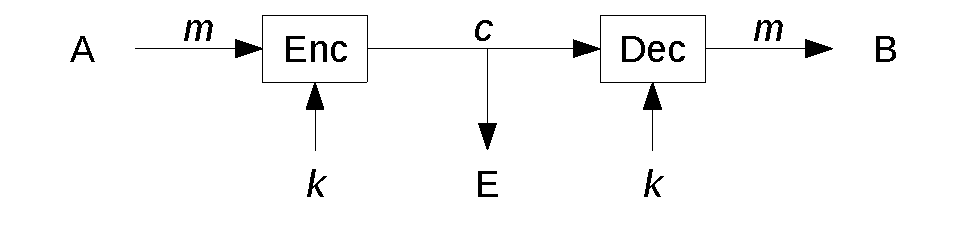
\includegraphics[width=0.8\linewidth]{drawings/symmetric-encryption.eps}
	\caption{Message exchange between $A$ and $B$ using symmetric encryption. $E$ is the eavesdropper.}
	\label{fig:symmetric-encryption}
\end{figure}

Our encryption schemes have the following syntax:
\begin{equation*}
	\GenericEncSchemeTuple.
\end{equation*}
$A$ and $B$, the actors of our communication exchange (\cref{fig:symmetric-encryption}), share $k$, the key, taken from some key space $\K$.
The elements of our encryption scheme play the following roles:
\begin{enumerate}
	\item $\GenericKeyGen$ outputs a random key from the key space $\K$, and we write this as $k \leftarrow \GenericKeyGen(1^n)$ with $1^n$ where $n$ will quantify the security of the cipher;
	\item $\GenericEnc : \K \times \M \to \C$ is the encryption function, mapping a key and a message to a cyphertext\footnote{In cryptography, ciphertext or cyphertext is the result of encryption performed on plaintext using an algorithm, called a cipher. Ciphertext is also known as encrypted or encoded information because it contains a form of the original plaintext that is unreadable by a human or computer without the proper cipher to decrypt it.}. Given a message to be encrypted $m \in \M$ and the shared key $k$ calculate the cryptotext $c = \GenericEnc(m)$;
	\item $\GenericDec : \K \times \C \to \M$ is the decryption function, mapping a key and a cyphertext to a message. Given a cryptotext $c$ and the shared key $k$ returns the message $m \in \M$ such that $m = \GenericDec(c)$.
\end{enumerate}
We expect an encryption scheme to be at least correct and for each $n$, for each key $k \leftarrow \GenericKeyGen(1^n)$ and for every message $m \in \M$ we have:
\begin{equation*}
	\forall k \in \K, \forall m \in \M . \GenericDec(k, \GenericEnc(k, m)) = m.
\end{equation*}
An encryption scheme is defined by three algorithms $\GenericKeyGen$, $\GenericEnc$, and $\GenericDec$, as well as a specification of a message space $\M$ with $| \M | > 1$.\footnote{If $| M | = 1$ there is only one message and there is no point in communicating, let alone encrypting.}
\section{Perfect secrecy}

Shannon defined ``perfect secrecy'', \ie we will require that the adversary is not able to obtain any additional information about $m$. Formally we can express this request through probability theory.
\begin{definition}[Perfect secrecy]\label{def:perfect-secrecy}
	Let $M$ be a \ac{RV} over $\M$, and $K$ be a uniform distribution over $\K$.

	$(\GenericEnc, \GenericDec)$ has perfect secrecy if, $\forall m \in \M$ and $\forall c \in \C$ such that $\Pr {C = c} \geq 0$ \footnote{This requirement is necessary only to avoid influencing an event with zero probability. In the following we will always assume that $\Pr {M = m}$ and $\Pr {C = c}$ are positive. What has been shown can be generalized to the case of arbitrary distributions on $\M$ and $\C$.}:
	\begin{equation*}
		\forall M, \forall m \in \M, c \in \C . \Pr{M = m} = \Pr{M = m | C = c}
	\end{equation*}
	where $C = \GenericEnc(k,m)$ is a third \ac{RV}.
\end{definition}

We have equivalent definitions for perfect secrecy.
\begin{theorem}\label{thm:perfect-secrecy:equivalent-definitions}
	The following definitions are equivalent:
	\begin{enumerate}
		\item \label{itm:thm:perfect-secrecy:original} \cref{def:perfect-secrecy}: $\forall m \in \M$ and $\forall c \in \C$:
		\begin{equation*}
			\Pr{M = m} = \Pr{M = m | C = c}
		\end{equation*}
		\item \label{itm:thm:perfect-secrecy:independent} $\forall m \in \M$ and $\forall c \in \C$ $M$ and $C$ are independent;
		\item \label{itm:thm:perfect-secrecy:invariant}
		$\forall m, m' \in \M, \forall c \in \C \quad \footnote{The encryption algorithm may be probabilistic, so that $\GenericEnc(m)$ might output a different ciphertext when run multiple times. To emphasize this, we write $c \leftarrow \GenericEnc(m)$ to denote the possibly probabilistic process by which message $m$ is encrypted using key $k$ to give ciphertext $c$.}:$
			\begin{equation*}
				\Pr{\GenericEnc(k,m) = c} = \Pr{\GenericEnc(k,m') = c}
			\end{equation*}
			where $k$ is a random key in $\K$ chosen with uniform probability. \qedhere
	\end{enumerate}
\end{theorem}

It is sufficient to show that $(1) \Rightarrow (2) \Rightarrow (3) \Rightarrow (1)$




\begin{tcolorbox}[colframe=black, colback=sfondo_gray, sharp corners]
	
We can express the relationship between joint and marginal densities through the concept of \textit{conditional discrete density}. The probability of event $\mathcal{E}_1$ conditional on event $\mathcal{E}_2$ is the probability that event $\mathcal{E}_1$ occurs given that $\mathcal{E}_2$ occurs. For example, returning to the example of the die, the probability of getting a $\spadesuit$ knowing that the result of the roll will be $\spadesuit$ or $\heartsuit$ is $1/3$. Formally, we have:

\[
\Pr{\mathcal{E}_1 \mid \mathcal{E}_2} = \frac{\Pr{\mathcal{E}_1 \land \mathcal{E}_2}}{\Pr{\mathcal{E}_2}}.
\]

Two events are said to be \textit{statistically independent} when $\Pr{\mathcal{E}_1 \mid \mathcal{E}_2} = \Pr{\mathcal{E}_1}$ (i.e., when the probability that $\mathcal{E}_1$ occurs given that $\mathcal{E}_2$ occurs is equal to the probability that $\mathcal{E}_1$ occurs a priori). The relationship between $\Pr{\mathcal{E}_1 \mid \mathcal{E}_2}$ and $\Pr{\mathcal{E}_2 \mid \mathcal{E}_1}$ is given by Bayes' theorem, expressed by the following equation:

\[
\Pr{\mathcal{E}_2 \mid \mathcal{E}_1} = \Pr{\mathcal{E}_1 \mid \mathcal{E}_2} \cdot \frac{\Pr{\mathcal{E}_2}}{\Pr{\mathcal{E}_1}} \tag{A.3}
\]

Switching to densities, given two random variables $X \in \mathcal{X}$ and $Y \in \mathcal{Y}$, the conditional probability of $Y = y$ given $X = x$ is:
\begin{proof}
\[
\Pr{Y = y \mid X = x} = \frac{\Pr{X = x \land Y = y}}{\Pr{X = x}} \stackrel{\text{(A.3)}}{=} \frac{\Pr{Y = y \mid X = x} \Pr{Y = y}}{\Pr{X = x}}
\]
\end{proof}
\end{tcolorbox}


\begin{proof}[Proof of \cref{thm:perfect-secrecy:equivalent-definitions}]
	First, we show that \ref{itm:thm:perfect-secrecy:original} $\implies$ \ref{itm:thm:perfect-secrecy:independent}.
	\begin{align*}
		\Pr{M=m} & = \Pr{M = m | C = c} \\
		& = \frac{\Pr{M = m \land C = c}}{\Pr{C = c}} \tag{by Bayes}
		\\
		& \implies \\
		\Pr{M = m} \Pr{C = c}
		& =
		\Pr{M = m \land C = c}
	\end{align*}
	which is the definition of independence \footnote{In the context of probability theory: Both \( \land \) and \( \cap \) serve the purpose of indicating the intersection of events. The choice between \( \land \) and \( \cap \) may vary based on personal preference or the context in which it's used, but they convey the same meaning in probability theory.}.

	Now we show that \ref{itm:thm:perfect-secrecy:independent} $\implies$ \ref{itm:thm:perfect-secrecy:invariant}.
	\begin{align*}
		\Pr{\GenericEnc(k, m) = c} 
		& =
		\Pr{\GenericEnc(k, M) = c | M = m} \tag{we fixed $m$}
		\\
		& = \Pr{C = c | M = m} \tag{definition of the \ac{RV} $C$}
		\\
		& = \Pr{C = c}. \tag{by \ref{itm:thm:perfect-secrecy:independent}}
	\end{align*}
	Since $m$ is arbitrary, we can do the same for $m'$, and obtain
	\begin{equation*}
		\Pr{\GenericEnc(k,m') = c} = \Pr{C = c}
	\end{equation*}
	which gives us \ref{itm:thm:perfect-secrecy:invariant}.

	Now we want to show that \ref{itm:thm:perfect-secrecy:invariant} $\implies$ \ref{itm:thm:perfect-secrecy:original}. Assume that the encryption scheme is perfectly secret and fix messages $m$, $m\prime$ $\in \M$ and a ciphertext $c \in \C$. Take any $c \in \C$. By \ref{itm:thm:perfect-secrecy:independent} we have:

	\begin{equation*}
		\Pr {C = c | M = m} = \Pr {C = c} = \Pr {C = c | M = m'}.
	\end{equation*}

	completing the proof of the first direction.
	Assume next that for every distribution over $\M$, every $m$, $m\prime \in \M$, and every $c \in \C$ it holds that $\Pr {C = c | M = m} = \Pr {C = c | M = m\prime}$. Fix some distribution over $\M$, and an arbitrary $m \in \M$ and $c \in \C$. Define $p \stackrel{\text{def}}{=}$ $\Pr {C = c | M = m}$. Since $\Pr {C = c | M = m} = \Pr {C = c | M = m'} = p$ for all $m$, we have:

	\begin{align*}
		\Pr{C = c}
		& =
		\sum_{m' \in \M} \Pr{C = c \land M = m'}
		\\
		& = 
		\sum_{m' \in \M} \Pr{C = c | M = m'} \Pr{M = m'}
		\tag{by Bayes}
		\\
		& =
		\sum_{m' \in \M} \Pr{\GenericEnc(k,M) = c | M = m'} \Pr{M = m'}
		\\
		& =
		\sum_{m' \in \M} \Pr{\GenericEnc(k,m') = c} \Pr{M = m'}
		\\
		& =
		\Pr{\GenericEnc(k, m) = c} \underbrace{\sum_{m' \in \M} \Pr{M = m'}}_{1}
		\tag{$\GenericEnc$ is indepenendent of $M$, so we take it out}
		\\
		& =
		\Pr{\GenericEnc(k,M) = c | M = m} =
		\Pr{C = c | M = m}.
	\end{align*}
	We are left to show that $\Pr{M = m} = \Pr{M = m | C = c}$, but this is easy with Bayes.
\end{proof}


\begin{theorem}(Shannon Theorem)
	Let $|\M| = |\K| = |\C|$. A cipher has perfect secrecy if and only if:
	\begin{enumerate}[label=(\roman*)]
		\item Each key $k \in \K$ is chosen uniformly with probability $\frac{1}{|\K|}$;
		\item For every message $m \in \M$ and every ciphertext $c \in \C$, there exists one and only one key $k$ such that $c = \GenericKeyGen(m)$.
	\end{enumerate}
\end{theorem}

\section{\acl{OTP} (Vernam's Cipher)}

Now we'll see a perfect encryption scheme, the \ac{OTP}.



\begin{tcolorbox}[colframe=black, colback=sfondo_gray, sharp corners]

\begin{construction}[\acl{OTP}]
	The message space, the cyphertext space, and the key space are all the same, \ie $\M = \K = \C = \{0,1\}^{l}$, with $l \in \Naturals$.

	The \acl{OTP} encryption scheme by Vernam is defined as follows:
	
	\begin{itemize}
		\item Fix an integer $l$ $>$ 0. Then the message space $\M$, key space $\K$, and ciphertext space $\C$ are all equal to $\{0, 1\}^l$ (i.e., the set of all binary strings of length $l$);
		\item The key-generation algorithm $\GenericKeyGen$ works by choosing a string from $\K = \{0, 1\}^l$ according to the uniform distribution (i.e., each of the $2^l$ strings in the space is chosen as the key with probability exactly $2^{-l}$). Generate a random key $k \leftarrow \{0,1\}^l$;
		\item $\GenericEnc$: to encrypt the message \( m \in \{0, 1\}^l \), we define:
		\begin{equation*}
			c = \text{Enc}(m) = k \oplus m
		\end{equation*}
		\item $\GenericDec$: To decrypt the ciphertext $c \in \{0, 1\}^l$ with key $k$ compute:
		\begin{equation*}
			m = \text{Dec}(c) = c \oplus k
		\end{equation*}
	\end{itemize}
\end{construction}
\end{tcolorbox}
Seeing that this is correct is immediate.

This can actually be done in any finite abelian\footnote{An abelian group, also known as a commutative group, is a fundamental concept in abstract algebra where the group's binary operation (commonly denoted as \(+\) or multiplication in different contexts) is commutative. This means that the order of elements in the operation does not affect the result. Examples include additive groups of integers (\(\mathbb{Z}\)), rational numbers (\(\mathbb{Q}\)), and multiplicative groups of non-zero rational numbers (\(\mathbb{Q}^*\)), as well as matrix groups with matrix multiplication. Abelian groups play a crucial role in abstract algebra, with many theorems and concepts specifically applying to them.
} group $(\Group, +)$, where you just do $k + m$ to encode and $c - k$ to decode.


\begin{theorem} \label{thm:otp:perfect-secrecy}
	\ac{OTP} is perfectly secure.
\end{theorem}

\begin{proof}[Proof of \cref{thm:otp:perfect-secrecy}]
	Fix $m \in \M, c \in \C$, and choose a random key.
	\begin{equation*}
		\Pr{\OTPEnc(k,m) = c} = \Pr{k = c - m} = \frac{1}{\abs{\Group}}.
	\end{equation*}
	This is true for any $m$, so we are done.
\end{proof}

\ac{OTP} has two problems:
\begin{enumerate}
	\item the key is long (as long as the message);
	\item we can't reuse the key:
	\begin{equation*}
		\begin{array}{c}
			c = k + m \\
			c' = k + m'
		\end{array}
		\implies
		k = c - m = c' - m'
		\implies
		m' = m - (c - c').
	\end{equation*}
\end{enumerate}

\begin{theorem}[Shannon, 1949] \label{thm:shannon:1949}
	In any perfectly secure encryption scheme the size of the key space is at least as large as the size of the message space, \ie $\abs{\K} \ge \abs{\M}$.
\end{theorem}

\begin{proof}[Proof of \cref{thm:shannon:1949}]
	Assume, for the sake of contradiction, that $\abs{\K} < \abs{\M}$.
	Fix $M$ to be the uniform distribution over $\M$, which we can do as perfect secrecy works for any distribution.
	Take a cyphertext $c \in \C$ such that $\Pr{C = c} > 0$, \ie $\exists m, k$ such that $\OTPEnc(k,m) = c$.

	Consider $\M' = \{ \OTPDec(k,c) : k \in \K \}$, the set of all messages decrypted from $c$ using any key.
	Clearly, $\abs{\M'} \le \abs{\K} < \abs{\M}$, so $\exists m' \in \M$ such that $m' \not\in \M'$.
	This means that
	\begin{equation*}
		\Pr{M = m'} = \frac{1}{\abs{\M}} \neq \Pr{M = m' | C = c} = 0
	\end{equation*}
	in contradiction with perfect secrecy.
\end{proof}

In the rest of the course we will forget about perfect secrecy, and strive for computational security, \ie bound the computational power of the adversary.

\section{Authentication}

The aim of authentication is to avoid tampering of $E$ with the messages exchanged between $A$ and $B$ (\cref{fig:symmetric-authentication}).

\begin{figure}
	\centering
	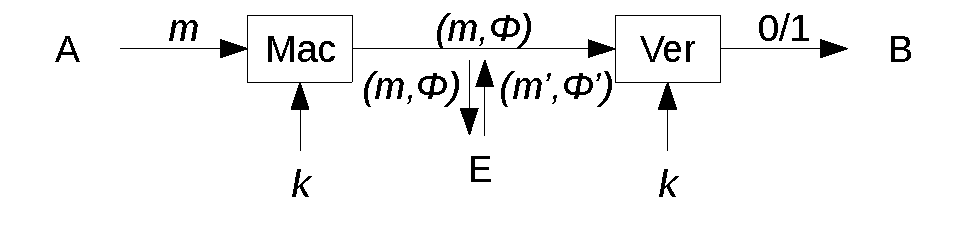
\includegraphics[width=0.8\linewidth]{drawings/symmetric-authentication.eps}
	\caption{Message exchange between $A$ and $B$ using symmetric authentication. $E$ is the eavesdropper.}
	\label{fig:symmetric-authentication}
\end{figure}

A \ac{MAC} is defined as a tuple $\GenericMACSchemeTuple$, where:
\begin{itemize}
	\item $\GenericKeyGen$, as usual, outputs a random key from some key space $\K$;
	\item $\GenericMac : \K \times \M \to \GenericAuthSpace$ maps a key and a message to an authenticator in some authenticator space $\GenericAuthSpace$;
	\item $\GenericVrfy : \K \times \M \times \GenericAuthSpace \to \Bool$ verifies the authenticator.
\end{itemize}
As usual, we expect a \ac{MAC} to be correct, \ie
\begin{equation*}
	\forall m \in \M, \forall k \in \K . \GenericVrfy(k, m, \GenericMac(k, m)) = 1.
\end{equation*}

If the $\GenericMac$ function is deterministic, then it must be that $\GenericVrfy(k, m, \phi) = 1$ if and only if $\GenericMac(k, m) = \phi$.

Security for \acp{MAC} is that \emph{forgery} must be hard: you can't come up with an authenticator for a message if you don't know the key.

\begin{definition}[Information theoretic \acs{MAC}]
	$(\GenericMac, \GenericVrfy)$ has $\epsilon$-statistical security if for all (possibly unbounded) adversary $\Adv$, for all $m \in \M$,
	\begin{equation*}
		\Pr{
			\GenericVrfy(k, m', \phi') = 1 \land m' \neq m :
			\begin{array}{l}
				k \rand{\KeyGen}; \; \\
				\phi = \GenericMac(k,m); \; \\
				(m', \phi') \from \Adv(m,\phi)
			\end{array}
		} \le \epsilon
	\end{equation*}
	\ie the adversary forges a $(m',\phi')$ that verifies with key $k$ with low probability, even if it knows a valid pair $(m, \phi)$.
\end{definition}

As an exercise, prove that the above is impossible if $\epsilon = 0$.

Information theoretic security is also called unconditional security.
Later we'll see \emph{conditional} security, based on computational assumptions.

\begin{definition}[Pairwise independence]
	Given a family $\H = \{ h_k : \M \to \GenericAuthSpace \}_{k \in \K}$ of functions, we say that $\H$ is pairwise independent if for all distinct $m, m'$ we have that $(h_k(m), h_k(m')) \in \GenericAuthSpace^2$ is uniform over the choice of $k \rand{\K}$.
\end{definition}

We show straight away a construction of a pairwise independent family of function.
\begin{construction}[Pairwise independent function] \label{cons:pairwise-independent}
	Let $p$ be a prime, the functions in our family $\H$ are defined as
	\begin{equation*}
		h_{a,b}(m) = a m + b \mod p
	\end{equation*}
	with $\K = \Integers^2_p$, and with $\M = \GenericAuthSpace = \Integers_p$.
\end{construction}

\begin{theorem} \label{thm:mod-pairwise-independent}
	\Cref{cons:pairwise-independent} is pairwise independent.
\end{theorem}

\begin{proof}[Proof of \cref{thm:mod-pairwise-independent}]
	For any $m, m'$, $\phi, \phi'$, we want to find the value of
	\begin{equation*}
		\Pr{a m + b = \phi \land a m' + b = \phi'}
	\end{equation*}
	for $a,b \rand{\Integers^2_p}$.
	This is the same as
	\begin{equation*}
		\Pr[a,b]{
			\begin{pmatrix}
				m & 1 \\
				m' & 1
			\end{pmatrix}
			\begin{pmatrix}
			a \\ b
			\end{pmatrix}
			=
			\begin{pmatrix}
			\phi \\ \phi'
			\end{pmatrix}
		}
		=
		\Pr[a,b]{
			\begin{pmatrix}
			a \\ b
			\end{pmatrix}
			=
			{
			\begin{pmatrix}
				m & 1 \\
				m' & 1
			\end{pmatrix}
			}^{-1}
			\begin{pmatrix}
			\phi \\ \phi'
			\end{pmatrix}
		}
		=
		\frac{1}{\abs{\GenericAuthSpace}^2}.
	\end{equation*}
	This is true since 
	${\begin{psmallmatrix}
		m & 1 \\
		m' & 1
	\end{psmallmatrix}
	}^{-1}
	\begin{psmallmatrix}
	\phi \\ \phi'
	\end{psmallmatrix}$
	is just a couple of (constant) numbers, so the probability of choosing $(a,b)$ such that they equal the constant is just $\frac{1}{\abs{\GenericAuthSpace}^2}$.
\end{proof}

If $h_k$ is part of a pairwise independent family of functions, then $\GenericMac(k,m) = h_k(m)$, and $\GenericVrfy(k,m,\phi)$ is simply computing $h_k(m)$ and comparing it with $\phi$, \ie
\begin{equation*}
	\GenericVrfy(k,m,\phi) = 1 \iff h_k(m) = \phi.
\end{equation*}
We now prove that this is an information theoretic \ac{MAC}.

\begin{theorem} \label{thm:pairwise-independent:statistical-security}
	Any pairwise independent function is $\frac{1}{\abs{\GenericAuthSpace}}$-statistical secure.
\end{theorem}

\begin{proof}[Proof of \cref{thm:pairwise-independent:statistical-security}]
	Take any two distinct $m, m'$, and two $\phi, \phi'$.
	We show that the probability that $\GenericMac(k,m') = \phi'$ is exponentially small.
	\begin{equation*}
		\Pr[k]{\GenericMac(k,m) = \phi} =
		\Pr[k]{h_k(m) = \phi} =
		\frac{1}{\abs{\GenericAuthSpace}}.
	\end{equation*}
	Now look at the joint probabilities:
	\begin{align*}
		\Pr[k]{\GenericMac(k,m) = \phi \land \GenericMac(k,m') = \phi'} 
		& = 
		\Pr[k]{h_k(m) = \phi \land h_k(m') = \phi'} 
		\tag{by definition}
		\\
		& =
		\frac{1}{\abs{\GenericAuthSpace}^2}
		=
		\frac{1}{\abs{\GenericAuthSpace}}
		\cdot
		\frac{1}{\abs{\GenericAuthSpace}}.
	\end{align*}
	The last steps come from the fact that $h_k$ is pairwise independent.
	To see that the construction is $\frac{1}{\abs{\GenericAuthSpace}}$-statistical secure:
	\begin{align*}
		\Pr[k]{\GenericMac(k, m') = \phi' | \GenericMac(k,m) = \phi}
		& =
		\Pr[k]{h_k(m') = \phi' | h_k(m) = \phi}
		\\
		& =
		\frac{\Pr[k]{h_k(m) = \phi \land h_k(m') = \phi'}}{\Pr[k]{h_k(m) = \phi}}
		\\
		& =
		\frac{1}{\abs{\GenericAuthSpace}}.
	\end{align*}
\end{proof}

Note that \cref{cons:pairwise-independent} ($h_k(m) = a m + b \mod p$) is insecure if the same key $k = (a,b)$ is used for two messages.

\begin{theorem}
	Any $t$-time $2^{-\lambda}$-statistically secure \ac{MAC} has key of size $(t+1)\lambda$.
\end{theorem}

\section{Randomness Extraction}

$X$ is a random source (possibly not uniform).
$\Ext(X) = Y$ is a uniform \ac{RV}.

First, let's see a construction for a binary \ac{RV}.
Let $B$ be a \ac{RV} such that $\Pr{B = 1} = p$ and $\Pr{B = 0} = 1-p$, with $p \neq 1-p$.
We take two samples, $B_1$ and $B_2$ from $B$, and we want to obtain an unbiased \ac{RV} $B'$.
\begin{enumerate}
	\item Take two samples, $b_1 \rand{B_1}$ and $b_2 \rand{B_2}$;
	\item if $b_1 = b_2$, sample again;
	\item if $(b_1 = 1 \land b_2 = 0)$, output 1; if $(b_1 = 0 \land b_2 = 1)$, output 0.
\end{enumerate}
It's easy to verify that $B'$ is uniform:
\begin{align*}
	\Pr{B' = 1} & = \Pr{B_1 = 1 \land B_2 = 0} = p (1-p) \\
	\Pr{B' = 0} & = \Pr{B_1 = 0 \land B_2 = 1} = (1-p) p.
\end{align*}
How many trials do we have to make before outputting something?
$2(1-p)p$ is the probability that we output something.
The probability that we don't output anything for $n$ steps is thus $(1 - 2(1-p)p)^n$.


% missing some stuff on randomness extraction

\pagebreak
\acresetall

\chapter{Computational Cryptography}


To introduce computational cryptography we first have to define a computational model.
We assume the adversary is efficient, \ie it is a \ac{PPT} adversary.

We want that the probability of success of the adversary is tiny, \ie negligible for some $\lambda \in \NaturalsZ$.
A function $\epsilon : \NaturalsZ \to \Reals$ is negligible if $\forall c > 0 . \exists n_0$ such that $\forall n > n_0 . \epsilon(n) < n^{-c}$.

We rely on computational assumptions, \ie in tasks believed to be hard for any efficient adversary.
In this setting we make conditional statements, \ie if a certain assumption holds then a certain crypto-scheme is secure.

\section{\aclp{OWF}}

A simple computational assumption is the existence of \acp{OWF}, \ie functions for which is hard to compute the inverse.

\begin{definition}[\acl{OWF}]
	A function $f : \{0,1\}^{\star} \to \{0,1\}^{\star}$ is a \ac{OWF} if $f(x)$ can be computed in polynomial time for all $x$ and for all $\ac{PPT}$ adversaries $\Adv$ it holds that
	\begin{equation*}
		\Pr{f(x') = y : x \rand{\{0,1\}^{\star}}; \; y = f(x); \; x' \from \Adv(1^{\lambda}, y)} \le \epsilon(\lambda). \qedhere
	\end{equation*}
\end{definition}

The $1^{\lambda}$ given to the adversary $\Adv$ is there to highlight the fact that $\Adv$ is polynomial in the length of the input ($\lambda$).

Russel Impagliazzo proved that \acp{OWF} are equivalent to One Way Puzzles, \ie couples $(\mathrm{Pgen}, \mathrm{Pver})$ where $\mathrm{Pgen}(1^{\lambda}) \to (y, x)$ gives us a puzzle ($y$) and a solution to it ($x$), while $\mathrm{Pver}(x,y) \to 0/1$ verifies if $x$ is a solution of $y$.

Another object of interest in this classification are average hard NP-puzzles, for which you can only get an instance, \ie $\mathrm{Pgen}(1^{\lambda}) \to y$.

Impagliazzo says we live in one of five worlds:
\begin{enumerate}
	\item Algorithmica, where P = NP;
	\item Heuristica, where there are no average hard NP-puzzles, \ie problems without solution;
	\item Pessiland, where you have average hard NP-puzzles;
	\item Minicrypt, where you have \ac{OWF}, one-way NP-puzzles, but no \ac{PKC};
	\item Cryptomania, where you have both \ac{OWF} and \ac{PKC}.
\end{enumerate}
We'll stay in Minicrypt for now.

\ac{OWF} are hard to invert on average.
Two examples:
\begin{itemize}
	\item factoring the product of two large prime numbers;
	\item compute the discrete logarithm, \ie take a finite group $(\Group, \cdot)$, and compute $y = g^x$ for some $g \in \Group$.
	The find $x = \log_{g}(y)$.
	This is hard to compute in some groups, \eg $\IntegersPrimeGroup$.
\end{itemize}

\section{Computational Indistinguishability}

\begin{definition}[Distribution Ensemble]
	A distribution ensemble $\X = \{ X_n \}_{n \in \NaturalsZ}$ is a sequence of distributions $X_i$ over some space $\{0,1\}^{\lambda}$.
\end{definition}

\begin{definition}[Computational Indistinguishability]
	Two distribution ensembles $\X_{\lambda}$ and $\Y_{\lambda}$ are computationally indistinguishable, written as $\X_{\lambda} \CompInd \Y_{\lambda}$, if for all \ac{PPT} distinguishers $\Distinguisher$ it holds that
	\begin{equation*}
		\abs{\Pr{\Distinguisher(\X_{\lambda}) = 1} - \Pr{\Distinguisher(\Y_{\lambda}) = 1}} \le \epsilon(\lambda).
	\end{equation*}
\end{definition}

\begin{lemma}[Reduction] \label{lem:reduction}
	If $\X \CompInd \Y$, then for all \ac{PPT} functions $f$, $f(\X) \CompInd f(\Y)$.
\end{lemma}

\begin{proof}[Proof of \cref{lem:reduction}]
	Assume, for the sake of contradiction, that $\exists f$ such that $f(\X) \not \CompInd f(\Y)$: then we can distinguish $\X$ and $\Y$.
	Since $f(\X) \not \CompInd f(\Y)$, then $\exists p = \poly(\lambda), \Distinguisher$ such that, for infinitely many $\lambda$s
	\begin{equation*}
		\abs{\Pr{\Distinguisher(f(\X_{\lambda})) = 1} - \Pr{\Distinguisher(f(\Y_{\lambda})) = 1}} \ge \frac{1}{p(\lambda)}.
	\end{equation*}

	$\Distinguisher$ distinguishes $\X_{\lambda}$ and $\Y_{\lambda}$ with non-negligible probability.
	Consider the following $\Distinguisher'$, which is given
	\begin{equation*}
		z =
		\begin{cases}
			x \rand{\X_{\lambda}}; \\
			y \rand{\Y_{\lambda}}. \\
		\end{cases}
	\end{equation*}
	$\Distinguisher'$ runs $\Distinguisher(f(z))$ and outputs whatever it outputs, and has the same probability of distinguishing $\X$ and $\Y$ of $\Distinguisher$, in contradiction with the fact that $\X \CompInd \Y$.
\end{proof}

Now we show that computational indistinguishability is transitive.

\begin{lemma}[Hybrid Argument] \label{lem:hybrid-argument}
	Let $\X = \{X_{\lambda}\}$, $\Y = \{ Y_{\lambda} \}$, $\Z = \{ Z_{\lambda} \}$ be distribution ensembles.
	If $\X_{\lambda} \CompInd \Y_{\lambda}$ and $\Y_{\lambda} \CompInd \Z_{\lambda}$, then $\X_{\lambda} \CompInd \Z_{\lambda}$.
\end{lemma}

\begin{proof}[Proof of \cref{lem:hybrid-argument}]
	This follows from the triangular inequality.
	\begin{align*}
		\abs{\Pr{\Distinguisher(\X_{\lambda}) = 1} - \Pr{\Distinguisher(\Z_{\lambda}) = 1}}
		= &~
		\left| \Pr{\Distinguisher(\X_{\lambda}) = 1} - \Pr{\Distinguisher(\Y_{\lambda}) = 1} \right.
		\\
		&~+
		\left. \Pr{\Distinguisher(\Y_{\lambda}) = 1} - \Pr{\Distinguisher(\Z_{\lambda}) = 1} \right|
		\\
		\le &~
		\abs{\Pr{\Distinguisher(\X_{\lambda}) = 1} - \Pr{\Distinguisher(\Y_{\lambda}) = 1}}
		\\
		&~+
		\abs{\Pr{\Distinguisher(\Y_{\lambda}) = 1} - \Pr{\Distinguisher(\Z_{\lambda}) = 1}}
		\\
		\le &~2 \epsilon(\lambda). \tag{negligible}
	\end{align*}
\end{proof}

We often prove $\X \CompInd \Y$ by defining a sequence $\H_0, \H_1, \dots, \H_t$ of distributions ensembles such that $\H_0 \equiv \X$ and $\H_t \equiv \Y$, and that for all $i$, $\H_i \CompInd \H_{i+1}$.

\section{\aclp{PRG}}

Let's see our first cryptographic primitive.
\acp{PRG} take in input a random seed and generate pseudo random sequences with some stretch, \ie output longer than input, and indistinguishable from a true random sequence.

\begin{definition}[\acl{PRG}]
	A function $\G : \{0,1\}^{\lambda} \to \{0,1\}^{\lambda + l(\lambda)}$ is a \ac{PRG} if and only if
	\begin{enumerate}
		\item $\G$ is computable in polynomial time;
		\item $\abs{\G(s)} = \lambda + l(\lambda)$ for all $s \in \{0,1\}^{\lambda}$;
		\item $\G \left( \U_{\lambda} \right) \CompInd \U_{\lambda + l(\lambda)}$.
	\end{enumerate}
\end{definition}

\begin{theorem} \label{thm:prg-any-stretch}
	If $\exists$ \ac{PRG} with 1 bit of stretch, then $\exists$ \ac{PRG} with $l(\lambda)$ bits of stretch, with $l(\lambda) = \poly(\lambda)$.
\end{theorem}

\begin{proof}[Proof of \cref{thm:prg-any-stretch}]
	We'll prove this just for some fixed constant $l(\lambda) = l \in \NaturalsZ$.

	\begin{figure}
		\centering
		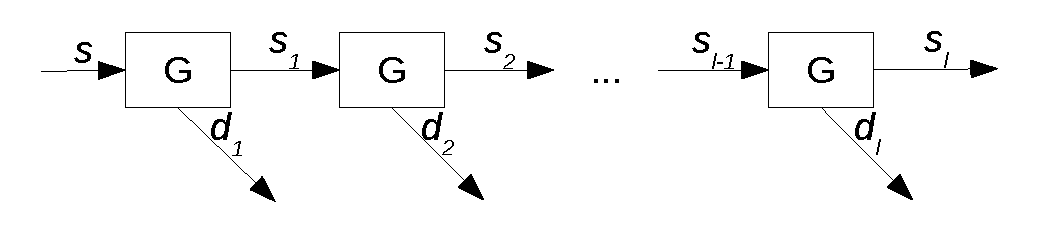
\includegraphics[width=0.8\linewidth]{drawings/prg-any-stretch.eps}
		\caption{Extending a \acs{PRG} with 1 bit stretch to a \acs{PRG} with $l$ bit stretch.}
		\label{fig:prg-any-stretch}
	\end{figure}

	First, let's look at the construction (\cref{fig:prg-any-stretch}).
	We replicate our \ac{PRG} $\G$ with 1 bit stretch $l$ times.
	The \ac{PRG} $\G^{l}$ that we define takes in input $s \in \{0,1\}^{\lambda}$, computes $(s_1, b_1) = \G(s)$, where $s_1 \in \{0,1\}^{l}$ and $b_1 \in \{0,1\}$, outputs $b_1$ and feeds $s_1$ to the second copy of \ac{PRG} $\G$, and so on until the $l$-th \ac{PRG}.

	To show that our construction is a \ac{PRG}, we define $l$ hybrids, with $\H_0^{\lambda} \equiv \G^{l}(\U_{\lambda})$, where $\G^{l} : \{0,1\}^{\lambda} \to \{0,1\}^{\lambda + l}$ is our proposed construction, and $\H_i^{\lambda}$ takes $b_1, \dots, b_i \rand{\{0,1\}}$, $s_i \rand{\{0,1\}^{\lambda}}$, and outputs $(b_1, \dots, b_i, s_l)$, where $s_l \in \{0,1\}^{\lambda + l - i}$ is $s_l = \G^{l-i}(s_i)$, \ie the output of our construction restricted to $l-i$ units.

	$\H_l^{\lambda}$ takes $b_1, \dots, b_l \rand{\{0,1\}}$ and $s_l \rand{\{0,1\}^{l}}$ and outputs $(b_1, \dots, b_l, s_l)$ directly.

	We need to show that $\H_i^{\lambda} \CompInd \H_{i+1}^{\lambda}$.
	To do so, fix some $i$.
	The only difference between the two hybrids is that $s_{i+1}, b_{i+1}$ are pseudo random in $\H_{i}^{\lambda}$, and are truly random in $\H_{i+1}^{\lambda}$.
	All bits before them are truly random, all bits after are pseudo random.

	Assume these two hybrids are distinguishable, then we can break the \ac{PRG}.
	Consider the \ac{PPT} function $f_i$ defined by $f(s_{i+1},b_{i+1}) = (b_1, \dots, b_l, s_l)$ such that $b_1, \dots b_i \rand{\{0,1\}}$ and, for all $j \in [i+1, l]$ $(b_j, s_j) = \G(s_{j-1})$.

	By the security of \acp{PRG} we have that $\G(\U_{\lambda}) \CompInd \U_{\lambda+1}$.
	By reduction, we also have that $f(\G(\U_{\lambda})) \CompInd f(\U_{\lambda+1})$.
	Thus, $\H_{i}^{\lambda} \CompInd \H_{i+1}^{\lambda}$.
\end{proof}

\section{\aclp{HCP}}

\begin{definition}[\acl{HCP} - I] \label{def:hcp-i}
	A polynomial time function $h : \{0,1\}^{n} \to \{0,1\}$ is \emph{hard core} for $f : \{0,1\}^{n} \to \{0,1\}^{n}$ if for all \ac{PPT} adversaries $\Adv$
	\begin{equation*}
		\Pr{\Adv(f(x)) = h(x) : x \rand{\{0,1\}^{n}}} \le \frac{1}{2} + \epsilon(\lambda).
	\end{equation*}
\end{definition}
The $\frac{1}{2}$ in the upper bound tells us that the adversary can't to better than guessing.

\begin{definition}[\acl{HCP} - II] \label{def:hcp-ii}
	A polynomial time function $h : \{0,1\}^{n} \to \{0,1\}$ is \emph{hard core} for $f : \{0,1\}^{n} \to \{0,1\}^{n}$ if for all \ac{PPT} adversaries $\Adv$
	\begin{equation*}
		\abs{
			\Pr{
			\begin{array}{c}
				\Adv(f(x), h(x)) = 1 : \\
				x \rand{\{0,1\}^{n}}
			\end{array}
			}
			-
			\Pr{
			\begin{array}{c}
				\Adv(f(x), b) = 1 : \\
				x \rand{\{0,1\}^{n}}; \\
				b \rand{\{0,1\}}
			\end{array}
			}
		}
		\le
		\epsilon(\lambda).
	\end{equation*}
\end{definition}

\begin{theorem}
	\Cref{def:hcp-i} and \cref{def:hcp-ii} are equivalent.
\end{theorem}
Proof of this theorem is left as exercise.

Luckily for us, every \ac{OWF} has a \ac{HCP}.
There isn't a single \ac{HCP} $h$ for all \acp{OWF} $f$.
Suppose $\exists$ such $h$, then take $f$ and let $f'(x) = h(x) || f(x)$.
Then, if $f'(x) = y || b$ for some $x$, it will always be that $h(x) = b$.

But, given a \ac{OWF}, we can create a new \ac{OWF} for which $h$ is hard core.

\begin{theorem}[\ac{GL}, 1983] \label{thm:gl}
	Let $f : \{0,1\}^n \to \{0,1\}^{n}$ be a \ac{OWF}, and define $g(x,r) = f(x) || r$ for $r \rand{\{0,1\}^{n}}$.
	Then $g$ is a \ac{OWF}, and 
	\begin{equation*}
		h(x,r) = \DotProduct{x}{r} = \sum_{i=1}^{n} x_i \cdot r_i \mod 2
	\end{equation*}
	is hardcore for $g$. 
\end{theorem}

\begin{definition}[\acl{OWP}]
	We say that $f : \{0,1\}^n \to \{0,1\}^{n}$ is a \ac{OWP} if $f$ is a \ac{OWF}, $\forall x . \abs{x} = \abs{f(x)}$, and for all distinct $x, x' . f(x) \neq f(x')$.
\end{definition}

\begin{corollary} \label{cor:owp-hcp-prg}
	Let $f$ be a \ac{OWP}, and consider $g : \{0,1\}^n \to \{0,1\}^{n}$ from the \ac{GL} theorem.
	Then $\G(s) = (g(s), h(s))$ is a \ac{PRG} with stretch 1.
\end{corollary}

\begin{proof}[Proof of \cref{cor:owp-hcp-prg}]
	\begin{align*}
		\G(\U_{2n})
		& =
		(g(x,r), h(x,r)) \\
		& =
		(f(x) || r, \DotProduct{x}{r}) \\
		& \CompInd 
		(f(x) || r, b) \tag{\ac{GL}}
		\\
		& \CompInd
		\U_{2n+1}.
	\end{align*}
\end{proof}

% this part is not clear

{\bfseries UNCLEAR}

Assume instead $f$ is a \ac{OWF}, and that is 1-to-1 (injective).
Consider $\X = g^m(\vec{x}) = (g(x_1), h(x_1), \dots, g(x_m), h(x_m))$, where $x_1, \dots, x_m \in \{0,1\}^{n}$ (\ie, $\vec{x} \in \{0,1\}^{nm}$).
You can construct a \ac{PRG} from a \ac{OWF} as shown by H.I.L.L.

\begin{fact}
$\X$ is indistinguishable from $\X'$ such that $\H_{\infty}(\X') \ge k = n \cdot m + m$, since $f$ is injective.
\end{fact}

Now $\G(s, \vec{x}) = (s, \Ext(s, g^{m}(\vec{x})))$ where $\Ext : \{0,1\}^{d} \times \{0,1\}^{nm} \to \{0,1\}^{l}$, and $l = nm + 1$.
This works for $m = \omega(\log(n))$.
You get extraction error $\epsilon \approx 2^{-m}$.


\pagebreak

\acresetall


\chapter{\acl{SKE} Schemes}

\begin{definition}[\acl{SKE} scheme]
	We call $\SKESchemeTuple$ a \ac{SKE} scheme.
	\begin{itemize}
		\item $\SKEKeyGen$ outputs a key $k \rand{\K}$;
		\item $\Enc(k, m) = c$ for some $m \in \M$, $c \in \C$;
		\item $\Dec(k, c) = m$.
	\end{itemize}
	As usual, we want $\SKEScheme$ to be correct.
\end{definition}

We want to introduce computational security: a bounded adversary can not gain information on the message given the cyphertext.
\begin{definition}[One time security]
	A \ac{SKE} scheme $\SKESchemeTuple$ has one time computational security if for all \ac{PPT} adversaries $\Adv$ $\exists$ a negligible function $\epsilon$ such that
	\begin{equation*}
		\abs{
			\Pr{\SKEGameOneTime(\lambda, 0) = 1}
			-
			\Pr{\SKEGameOneTime(\lambda, 1) = 1}
		}
		\le \epsilon(\lambda)
	\end{equation*}
	where $\SKEGameOneTime(\lambda, b)$ is the following ``game'' (or experiment):
	\begin{enumerate}
		\item pick $k \rand{\K}$;
		\item $\Adv$ outputs two messages $(m_0, m_1) \from \Adv(1^{\lambda})$ where $m_0, m_1 \in \M$ and $\abs{m_0} = \abs{m_1}$;
		\item $\c = \SKEEnc(k, m_b)$ with $b$ input of the experiment;
		\item output $b' \from \Adv(1^{\lambda}, c)$, \ie the adversary tries to guess which message was encrypted. \qedhere
	\end{enumerate}
\end{definition}

Let's look at a construction.
\begin{construction}[\acs{SKE} scheme from \acs{PRG}] \label{cons:ske-prg}
	Let $\G : \{0,1\}^{n} \to \{0,1\}^{l}$ be a \ac{PRG}.
	Set $\K = \{0,1\}^{n}$, and $\M = \C = \{0,1\}^{l}$.
	Define $\SKEEnc(k,m) = \G(k) \xor m$ and $\SKEDec(k,c) = \G(k) \xor c$.
\end{construction}

\begin{theorem} \label{thm:ske-prg}
	If $\G$ is a \ac{PRG}, the \ac{SKE} in \cref{cons:ske-prg} is one-time computationally secure.
\end{theorem}

\begin{proof}[Proof of \cref{thm:ske-prg}]
	Consider the following experiments:
	\begin{itemize}
		\item $\H_0(\lambda, b)$ is like $\SKEGameOneTime$:
		\begin{enumerate}
			\item $k \rand{\{0,1\}^{n}}$;
			\item $(m_0, m_1) \from \Adv(1^{\lambda})$;
			\item $c = \G(k) \xor m_b$;
			\item $b' \from \Adv(1^{\lambda}, c)$.
		\end{enumerate}
		\item $\H_1(\lambda, b)$ replaces $\G$ with something truly random:
		\begin{enumerate}
			\item $(m_0, m_1) \from \Adv(1^{\lambda})$;
			\item $r \rand{\{0,1\}^{l}}$;
			\item $c = r \xor m_b$, basically like \ac{OTP};
			\item $b' \from \Adv(1^{\lambda}, c)$.
		\end{enumerate}
		\item $\H_2(\lambda)$ is just randomness:
		\begin{enumerate}
			\item $(m_0, m_1) \from \Adv(1^{\lambda})$;
			\item $c \rand{\{0,1\}^{l}}$;
			\item $b' \from \Adv(1^{\lambda}, c)$.
		\end{enumerate}
	\end{itemize}

	First, we show that $\H_0(\lambda, b) \CompInd \H_1(\lambda, b)$, for $b \in \{0,1\}$.
	Fix some value for $b$, and assume exists a \ac{PPT} distinguisher $\Distinguisher$ between $\H_0(\lambda, b)$ and $\H_1(\lambda, b)$: we then can construct a distinguisher $\Distinguisher'$ for the \ac{PRG}.

	$\Distinguisher'$, on input $z$, which can be either $\G(k)$ for some $k \rand{\{0,1\}^{n}}$, or directly $z \rand{\{0,1\}^{l}}$, does the following:
	\begin{itemize}
		\item get $(m_0, m_1) \from \Distinguisher(1^{\lambda})$;
		\item feed $z \xor m_b$ to $\Distinguisher$;
		\item output the result of $\Distinguisher$.
	\end{itemize}

	Now, we show that $\H_1(\lambda, b) \CompInd \H_2(\lambda, b)$, for $b \in \{0,1\}$.
	By perfect secrecy of \ac{OTP} we have that $(m_0 \xor r) \approx z \approx (m_1 \xor r)$, so $\H_1(\lambda, 0) \CompInd H_2(\lambda) \CompInd \H_1(\lambda, 1)$.
\end{proof}

\begin{corollary}
	One-time computationally secure \ac{SKE} schemes are in Minicrypt.
\end{corollary}

This scheme is not secure if the adversary knows a $(m_1, c_1)$ pair, and we reuse the key.
Take any $m, c$, then $c \xor c_1 = m \xor m_1$, and you can find $m$.
This is called a \ac{CPA}, something we will defined shortly using a \ac{PRF}.

\section{\aclp{CPA} and \aclp{PRF}}

\begin{definition}[\acl{PRF}]
	Let $\F = \{ F_k : \{0,1\}^{n} \to \{0,1\}^{l} \}$ be a family of functions, for $k \in \{0,1\}^{\lambda}$.
	Consider the following two experiments:
	\begin{itemize}
		\item $\PRFGameReal(\lambda)$, defined as:
			\begin{enumerate}
				\item $k \rand{\{0,1\}^{\lambda}}$;
				\item $b' \from \Adv^{F_k(\cdot)}(1^{\lambda})$, where $\Adv$ can query an oracle for values of $F_k(\cdot)$, without knowing $k$.
			\end{enumerate}
		\item $\PRFGameRand(\lambda)$, defined as:
			\begin{enumerate}
				\item $R \rand{\R(n \to l)}$, \ie a function $R$ is chosen at random from all functions from $\{0,1\}^{n}$ to $\{0,1\}^{l}$;
				\item $b' \from \Adv^{R(\cdot)}(1^{\lambda})$, where $\Adv$ can query an oracle for values of $R(\cdot)$.
			\end{enumerate}
	\end{itemize}
	The family $\F$ of functions is a \ac{PRF} family if for all \ac{PPT} adversaries $\Adv$ $\exists$ a negligible function $\epsilon$ such that
	\begin{equation*}
		\abs{
			\Pr{\PRFGameReal(\lambda) = 1}
			-
			\Pr{\PRFGameRand(\lambda) = 1}
		}
		\le \epsilon(\lambda). \qedhere
	\end{equation*}
\end{definition}

To introduce \acp{CPA} and \ac{CPA}-secure \ac{SKE} schemes, we first introduce the game of \ac{CPA}.
As usual, a \ac{SKE} scheme is a tuple $\SKESchemeTuple$.

\begin{definition}[\acs{CPA}-secure \acs{SKE} scheme]
	Let $\SKESchemeTuple$ be a \ac{SKE} scheme, and consider the game $\CPAGame(\lambda, b)$, defined as:
	\begin{enumerate}
		\item $k \rand{\{0,1\}^{\lambda}}$;
		\item $(m_0, m_1) \from \Adv^{\SKEEnc(k, \cdot)} (1^{\lambda})$.
			$\Adv$ is given access to an oracle for $\SKEEnc(k, \cdot)$, so she knows some $(m,c)$ couples, with $c = \SKEEnc(k, m)$;
		\item $c \from \SKEEnc(k, m_b)$;
		\item $b' \from \Adv^{\SKEEnc(k, \cdot)}(1^{\lambda}, c)$.
	\end{enumerate}

	$\SKEScheme$ is \ac{CPA}-secure if for all \ac{PPT} adversaries $\Adv$
	\begin{equation*}
		\CPAGame(\lambda, 0) \CompInd \CPAGame(\lambda, 1). \qedhere
	\end{equation*}
\end{definition}

Deterministic schemes cannot achieve this, \ie when $\SKEEnc$ is deterministic the adversary could cipher $m_0$ and then compare $c$ to $\SKEEnc(k, m_0)$, and output $0$ if and only if $c = \SKEEnc(k, m_0)$.

Let's construct a \ac{CPA}-secure \ac{SKE} scheme using \acp{PRF}.
\begin{construction}[\acs{SKE} scheme from \acs{PRF}] \label{cons:ske-prf}
	Let $\F$ be a \ac{PRF}, we define the following \ac{SKE} scheme $\SKESchemeTuple$:
	\begin{itemize}
		\item $\SKEKeyGen$ takes $k \rand{\{0,1\}^{\lambda}}$;
		\item $\SKEEnc(k,m) = (r, F_k(r) \xor m)$, with $r \rand{\{0,1\}^{n}}$.
			Note that, since $F_k : \{0,1\}^{n} \to \{0,1\}^{l}$, we have that $\M = \{0,1\}^{l}$ and $\C = \{0,1\}^{n+l}$;
		\item $\SKEDec(k, (c_1, c_2)) = F_k(c_1) \xor c_2$. \qedhere
	\end{itemize}
\end{construction}

Our construction is both one time computationally secure, and secure against \acp{CPA}.
\begin{theorem} \label{thm:ske-prf-cpa}
	If $\F$ is a \ac{PRF}, \cref{cons:ske-prf} is \ac{CPA}-secure.
\end{theorem}

\begin{proof}[Proof of \cref{thm:ske-prf-cpa}]
	First, we define the experiment $\H_0(\lambda, b) \equiv \CPAGame(\lambda, b)$ as follows:
	\begin{enumerate}
		\item $k \rand{\{0,1\}^{\lambda}}$;
		\item $(m_0,m_1) \from \Adv^{\SKEEnc(k, \cdot)} (1^{\lambda})$;
		\item $c^{\star} \from (r^{\star}, F_k(r^{\star}) \xor m_b)$, where $r^{\star} \rand{\{0,1\}^{n}}$;
		\item output $b' \from \Adv^{\SKEEnc(k, \cdot)} (1^{\lambda}, c^{\star})$.
	\end{enumerate}
	Note that in the \ac{CPA} game the adversary has access to an encryption oracle using the chosen key.

	Now, for the first hybrid $\H_1(\lambda, b)$, where we sample a random function $R$ in place of $F_k$:
	\begin{enumerate}
		\item $R \rand{\R(n \to l)}$;
		\item $(m_0,m_1) \from \Adv^{\SKEEnc(R, \cdot)} (1^{\lambda})$, where now $\SKEEnc(R, m) = (r, R(r) \xor m)$ for some random $r$;
		\item $c^{\star} \from (r^{\star}, R(r^{\star}) \xor m_b)$, where $r^{\star} \rand{\{0,1\}^{n}}$;
		\item output $b' \from \Adv^{\SKEEnc(R, \cdot)} (1^{\lambda}, c^{\star})$.
	\end{enumerate}

	Our first claim is that $\H_0(\lambda, b) \CompInd \H_1(\lambda, b)$ for $b \in \{0,1\}$.
	As usual, we assume that exists an adversary $\Adv$ which can distinguish the experiments, \ie that can distinguish the oracles, and use $\Adv$ to create $\Adv_{\text{PRF}}$ that breaks the \ac{PRF}.

	$\Adv_{\text{PRF}}$ has access to some oracle $O(\cdot)$, with is one of two possibilities:
	\begin{equation*}
		O(x) =
		\begin{cases}
			F_k(x) & \text{ for } k \rand{\{0,1\}^{\lambda}} \\
			R(x) & \text{ for } R \rand{\R(n \to l)}.
		\end{cases}
	\end{equation*}
	$\Adv$ gives $\Adv_{\text{PRF}}$ some message $m$.
	$\Adv_{\text{PRF}}$ picks $r \rand{\{0,1\}^{n}}$, and queries $O(r)$ to get $z \in \{0,1\}^{l}$.
	Then it gives $(r, z \xor m)$ to $\Adv$.
	This is repeated as long as $\Adv$ asks for encryption queries.

	Then $\Adv$ gives to $\Adv_{\text{PRF}}$ $(m_0, m_1)$, which repeats the same procedure using $m_0$ as a message (to distinguish $\H_0(\lambda, 0)$ from $\H_1(\lambda, 0)$) to compute $c^{\star}$.
	$\Adv$, after receiving $c^{\star}$, asks some more encryption queries, and then outputs $b'$.
	If $b' = 1$, $\Adv_{\text{PRF}}$ says $R(\cdot)$, otherwise it says $F_k(\cdot)$.

	Now for the third experiment, $\H_2(\lambda)$, which uses $\PKEEnc(m) = (r_1, r_2)$ with $(r_1, r_2) \rand{\{0,1\}^{n+l}}$, \ie it outputs just randomness.

	Our second claim is that $\H_1(\lambda, b) \CompInd \H_2(\lambda)$ for $b \in \{0,1\}$.
	To see this, note that $\H_1$ and $\H_2$ are identical as long as collisions don't happen when choosing the $r$s.
	It suffices for us to show that collisions happen with small probability.

	Call $E_{i,j}$ the event ``random $r_i$ collides with random $r_j$''.
	The event of a collision is thus $E = \biglor_{i,j} E_{i,j}$, and its probability can be upper bounded as follows:
	\begin{equation*}
		\Pr{E} = \sum_{i,j} \Pr{E_{i,j}} = \sum_{i,j} \Coll\left(\U_n\right) \le \binom{q}{2} 2^{-n} \le \frac{q^{2}}{2^{n}}
	\end{equation*}
	where $q$ is the (polynomial) number of queries that the adversary does, and $\Coll\left(\U_n\right)$ is the probability of a collision when using a uniform distribution, which is $2^{-n}$.
\end{proof} 

\begin{theorem}[\acs{GGM}, 1982]
	\acp{PRF} can be constructed from \acp{PRG}.
\end{theorem}

\begin{corollary}
	\acp{PRF} are in Minicrypt.
\end{corollary}

\begin{construction}[\acs{GGM} tree] \label{cons:ggm-tree}
	Assume we have a length doubling \ac{PRG} $\G : \{0,1\}^{\lambda} \to \{0,1\}^{2\lambda}$.
	We say that $\G(x) \Definition (\G_0(x), \G_1(x))$ to distinguish the first $\lambda$ bits from the second $\lambda$ bits.

	\begin{figure}
		\centering
		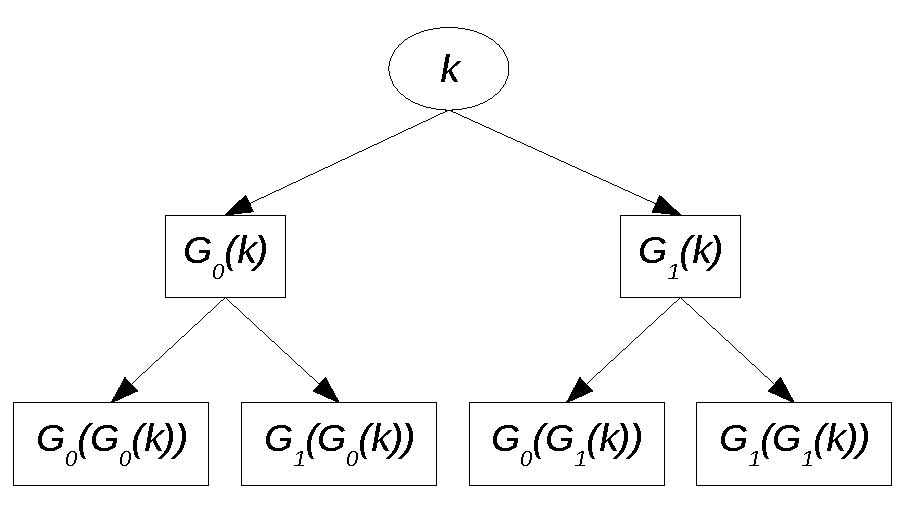
\includegraphics[width=0.8\linewidth]{drawings/ggm-tree.eps}
		\caption{First two levels of a \acs{GGM} tree.}
		\label{fig:ggm-tree}
	\end{figure}

	Now, to build the \ac{PRF} we construct a \ac{GGM} tree (\cref{fig:ggm-tree}) starting with a key $k \in \{0,1\}^{\lambda}$.
	On input $x = (x_1, \dots, x_n) \in \{0,1\}^{n}$, with $n$ being the height of the tree, the \ac{PRF} picks a path in the tree:
	\begin{equation*}
		F_k(x) = \G_{x_n} \left( \dots \G_{x_1}(k) \dots \right).
	\end{equation*}
\end{construction}

\begin{lemma} \label{lem:prg-poly-times}
	Let $\G : \{0,1\}^{\lambda} \to \{0,1\}^{2\lambda}$ be a \ac{PRG}.
	Then for all $t(\lambda) = \poly(\lambda)$ we have that
	\begin{equation*}
		\left( \G(k_1), \dots, \G(k_t) \right)
		\CompInd
		\underbrace{\left( \U_{2\lambda}, \dots, \U_{2\lambda} \right)}_{t \text{ times}}. \qedhere
	\end{equation*}
\end{lemma}

\begin{proof}[Proof of \cref{lem:prg-poly-times}]
	We define $t$ hybrids, where $\H_i(\lambda)$ is defined as
	\begin{equation*}
		\H_i(\lambda) = ( \G(k_1), \dots, \G(k_{t-i}), \underbrace{\U_{2\lambda}, \dots, \U_{2\lambda}}_{i \text{ times}} )
	\end{equation*}
	thus $\H_0(\lambda) = (\G(k_1), \dots, \G(k_t))$ and $\H_t(\lambda) = (\U_{2\lambda}, \dots, \U_{2\lambda})$.
	To prove that $\H_1(\lambda) \CompInd \H_t(\lambda)$, we show that for any $i$ it holds that $\H_i(\lambda) \CompInd \H_{i+1}(\lambda)$.
	This relies on the fact that $\G(k_{t-i}) \CompInd \U_{2\lambda}$: assume that exists a distinguisher $\Distinguisher$ for $\H_{i}(\lambda)$ and $\H_{i+1}(\lambda)$, we then break the \ac{PRG}.

	We build $\Distinguisher'$, which takes in input some $z$ from either $\G(k_{t-i})$ or $\U_{2\lambda}$.
	$\Distinguisher'$ takes $k_1, \dots, k_{t-(i+1)} \rand{\{0,1\}^{\lambda}}$, and feeds $(\G(k_1), \dots, \G(k_{t-(i+1)}), z, \U_{2\lambda}, \dots, \U_{2\lambda})$ to $\Distinguisher$, and returns whatever it returns.
\end{proof}

\begin{proof}[Proof that \cref{cons:ggm-tree} is a \acs{PRF}]
	We'll define a series of hybrids to show that the \ac{GGM} tree is a \ac{PRF}.
	$\H_0(\lambda) \equiv$ our \ac{GGM} tree.

	$\H_i(\lambda)$, for $i \in [1, n]$, will replace the tree up to depth $i$ with a true random function.
	$\H_i(\lambda)$ initially has two empty arrays $T_1$ and $T_2$.
	On input $x \in \{0,1\}^{n}$, it checks if $\vec{x} = (x_1, \dots, x_i) \in T_1$.
	If not, $\H_i(\lambda)$ picks $k_{\vec{x}} \rand{\{0,1\}^{\lambda}}$ and adds $\vec{x}$ to $T_1$ and $k_{\vec{x}}$ to $T_2$.
	If $\vec{x} \in T_1$, it just retrieves $k_{\vec{x}}$ from $T_2$.
	Then $\H_i(\lambda)$ outputs the following:
	\begin{equation*}
		\G_{x_n} \left( \G_{x_{n-1}} \left( \dots \G_{x_{i+1}} \left( k_{\vec{x}} \right) \dots \right) \right).
	\end{equation*}

	If $i = 0$ we have that $\vec{x} = \bot$ and that $k_{\bot} \rand{\{0,1\}^{\lambda}}$, so $\H_{0}(\lambda) \equiv$ the \ac{GGM} tree.
	On the other hand, if $i = n$, each input $x$ leads to a random output, so $\H_{n}(\lambda)$ is just a true random function.

	Assume now that exists an adversary $\Adv$ capable of telling apart $\H_{i}(\lambda)$ from $\H_{i+1}(\lambda)$, we could break the \ac{PRG}.
\end{proof}

\section{Computationally Secure \acsp{MAC}}

A computationally secure \ac{MAC} should be hard to forge, even if you see polynomially many authenticated messages.

\begin{definition}[\acs{UFCMA} \acs{MAC}]
	Let $\GenericMACSchemeTuple$ be a \ac{MAC}, and consider the game $\UFCMAGame(\lambda)$ defined as:
	\begin{enumerate}
		\item pick $k \rand{\{0,1\}^{\lambda}}$;
		\item $(m^{\star}, \phi^{\star}) \from \Adv^{\GenericMac(k, \cdot)}(1^{\lambda})$, where the adversary can query an authentication oracle;
		\item output $1$ if $\GenericVrfy(k, (m^{\star}, \phi^{\star})) = 1$ and $m^{\star}$ is ``fresh'', \ie it was never queried to $\GenericMac$.
	\end{enumerate}
	We say that $\GenericMACScheme$ is \ac{UFCMA} if for all \ac{PPT} adversaries $\Adv$ it holds that
	\begin{equation*}
		\Pr{\UFCMAGame (\lambda) = 1} \le \negl{\lambda}. \qedhere
	\end{equation*}
\end{definition}

As a matter of fact, any \ac{PRF} is a \ac{MAC}.

\begin{construction}[\acs{MAC} from \acs{PRF}] \label{cons:mac-prf}
	Let $\F = \{ F_k : \{0,1\}^{n} \to \{0,1\}^{l} \}_{k \in \{0,1\}^{\lambda}}$ be a \ac{PRF} family, and let $\K = \{0,1\}^{\lambda}$.
	Define $\GenericMac(k, m) = F_k(m)$.
\end{construction}

\begin{theorem} \label{thm:mac-prf-ufcma}
	If $\F$ is a \ac{PRF}, the \ac{MAC} shown in \cref{cons:mac-prf} is \ac{UFCMA}.
\end{theorem}

\begin{proof}[Proof of \cref{thm:mac-prf-ufcma}]
	Consider the game $\H(\lambda)$ where:
	\begin{enumerate}
		\item $R \rand{\R(n \to l)}$ is a random function;
		\item $(m^{\star}, \phi^{\star}) \from \Adv^{R(\cdot)} (1^{\lambda})$;
		\item output $1$ if $R(m^{\star}) = \phi^{\star}$ and $m^{\star}$ is ``fresh''.
	\end{enumerate}
	Our first claim is that $\H(\lambda) \CompInd \UFCMAGame(\lambda)$ for all \ac{PPT} adversaries $\Adv$.
	Assume not, then $\exists$ a distinguisher $\Distinguisher$ for $\H(\lambda)$ and $\UFCMAGame(\lambda)$, and we can construct a distinguisher $\Distinguisher'$ for the \ac{PRF}.
	$\Distinguisher'$ has access to an oracle $O(\cdot)$ which is either $F_k(\cdot)$ for some random $k$, or $R(\cdot)$ for some random function $R$.
	$\Distinguisher'$ feeds a game to $\Distinguisher$ using $O(\cdot)$.

	Our second claim is that $\Pr{\H(\lambda) = 1} \le 2^{-\lambda}$, since $R(\cdot)$ is random and the only way to predict it is by guessing.
\end{proof}

Up to this point we have shown that \ac{OWF}, \ac{PRG}, \ac{PRF} and \ac{MAC} are all in Minicrypt.

\section{Domain Extension}

We look now at domain extension.
Suppose we have a \ac{PRF} family $\F = \{ F_k : \{0,1\}^{n} \to \{0,1\}^{l}\}$ as above, and we have a message $m = m_1 || \dots || m_t$, with $m_i \in \{0,1\}^{n}$, and with $t$ being the number of blocks of $m$.

Let's look at some constructions that won't work.
\begin{enumerate}
	\item $\phi = \GenericMac\left(k, \bigxor_{i=1}^{t} m_i\right)$ does not work, since with $m = m_1 || m_2$ we could swap the bits in position $i$ of $m_1$ and $m_2$ and have the same authenticator;
	\item $\phi_i = \GenericMac(k, m_i)$ and $\phi = \phi_1 || \dots || \phi_t$ does not work, since we could rearrange the blocks of the authenticator and of the message and still get a valid couple. \ie take $m' = m_1 || m_3 || m_2$ and $\phi' = \phi_1 || \phi_3 || \phi_2$;
	\item $\phi_i = \GenericMac(k, \repr{i} || m_i)$ and $\phi = \phi_1 || \dots || \phi_t$, where $\repr{i}$ is the binary representation of integer $i$, does not work, since we could cut and paste blocks from different message/authenticator couples and to get a fresh valid couple.
\end{enumerate}

Now, for the real one.
To extend the domain of a \ac{PRF} $\F$ we need a function $h : \{0,1\}^{nt} \to \{0,1\}^{n}$ for which is hard to find a collision, \ie two distinct messages $m', m''$ such that $h(m') = h(m'')$.
To do this, we introduce \acp{CRH}, an object found in Cryptomania.
We add a key to the hash function.

\begin{definition}[\acl{UHF}]
	The family of functions $\H = \{ h_s : \{0,1\}^{N} \to \{0,1\}^{n} \}_{s \in \{0,1\}^{\lambda}}$ is universal (as in \ac{UHF}) if for all distinct $x, x'$ we have that
	\begin{equation*}
		\Pr[s \rand{\{0,1\}^{\lambda}}]{h_s(x) = h_s(x')} \le \epsilon.
	\end{equation*}
	Two cases are possible, depending on what $\epsilon$ is:
	\begin{itemize}
		\item if $\epsilon = 2^{-n}$, then $\H$ is said to be \ac{PU};
		\item if $\epsilon = \negl{\lambda}$, with $\lambda = \abs{s}$, then $\H$ is said to be \ac{AU}. \qedhere
	\end{itemize}
\end{definition}

With \ac{UHF} we can extend the domain of a \ac{PRF}.
\begin{theorem} \label{thm:uhf-prf-extension}
	If $\F$ is a \ac{PRF} and $\H$ is a \ac{AU} family of hash functions, then $\F(\H)$, defined as
	\begin{equation*}
		\F(\H) = \left\{ F_k(h_s(\cdot)) : \{0,1\}^{N} \to \{0,1\}^{l} \right\}_{k' = (k,s)}
	\end{equation*}
	is a \ac{PRF}.
\end{theorem}

\begin{proof}[Proof of \cref{thm:uhf-prf-extension}]
	Consider the following games:
	\begin{itemize}
		\item $\UHFGameReal(\lambda)$, defined as:
		\begin{enumerate}
			\item $k \rand{\{0,1\}^{\lambda}}$, $s \rand{\{0,1\}^{\lambda}}$;
			\item $b' \from \Adv^{F_k(h_s(\cdot))} (1^{\lambda})$.
		\end{enumerate}
		\item $\UHFGameRand(\lambda)$, defined as:
		\begin{enumerate}
			\item $\overline{R} \rand{\R(N \to l)}$;
			\item $b \from \Adv^{\overline{R}(\cdot)} (1^{\lambda})$.
		\end{enumerate}
	\end{itemize}

	Consider also the hybrid $\UHFGameHybrid(\lambda)$:
	\begin{enumerate}
		\item $s \rand{\{0,1\}^{\lambda}}$;
		\item $R \rand{R(n \to l)}$;
		\item $b \from \Adv^{R(h_s(\cdot))} (1^{\lambda})$.
	\end{enumerate}

	The first claim, \ie that $\UHFGameReal(\lambda) \CompInd \UHFGameHybrid(\lambda)$, is left as exercise.

	The second claim is that $\UHFGameHybrid(\lambda) \CompInd \UHFGameRand(\lambda)$.
	Assume the adversary asks $q$ distinct queries.
	Consider the event $E$ = ``$\exists (x_i, x_j)$ such that $h_s(x_i) = h_s(x_j)$ with $i \neq j$'', and with $i,j \le q$. 
	If $E$ doesn't happen, $\UHFGameHybrid(\lambda)$ and $\UHFGameRand(\lambda)$ are the same.
	This event is the same as getting first all the inputs that the adversary wants to try, and then sampling $s \rand{\{0,1\}}^{\lambda}$, so its probability can be bounded as
	\begin{equation*}
		\Pr{E} = \Pr{\exists i,j : h_s(x_i) = h_s(x_j)} \le \binom{q}{2} \epsilon \le q^2 \epsilon. \qedhere
	\end{equation*}
\end{proof}

Now, let's look at a construction.
\begin{construction}[\acs{UHF} with Galois field]
	Let $\Field$ be a finite field, such as the Galois field over $2^n$.
	In the Galois field, a bit string represents the coefficients of a polynomial of degree $n-1$.
	Addition is the usual, while for multiplication an irreducible polynomial $p(x)$ of degree $n$ is fixed, and the operation is carried out modulo $p(x)$.

	We pick $s \in \Field$, and $x = x_1 || \dots || x_t$ with $x_i \in \Field$ for all $i$.
	The hash function is defined as
	\begin{equation*}
		h_s(x) = h_s(x_1 || \dots || h_t) =
		\sum_{i=1}^{t} x_i \cdot s^{i-1} = Q_x(s).
	\end{equation*}
	A collision is two distinct $x, x'$ such that
	\begin{equation*}
		Q_x(s) = Q_{x'}(s) \iff Q_{x-x'}(s) = 0 \iff \sum_{i=1}^{t} (x_i - x_i') s^{i-1} = 0.
	\end{equation*}
	This means that $s$ is a root of $Q_{x-x'}$.
	So the probability of a collision is:
	\begin{equation*}
		\Pr{h_s(x) = h_s(x')} = \frac{t-1}{\abs{\Field}} = \frac{t-1}{2^n}. \tag{negligible}
	\end{equation*}
\end{construction}

We now look at a computational variant of hash functions.
We want hash functions for which collisions are difficult to find for any \ac{PPT} adversary $\Adv$, \ie families of functions such that
\begin{equation*}
	\Pr[s]{h_s(x) = h_s(x') : (x,x') \from \Adv (1^{\lambda})} \le \epsilon.
\end{equation*}

We want to use some \ac{PRF} family $\F$ to define $\H$.
Enter \ac{CBC}-\ac{MAC} (\cref{fig:cbc-mac}).
\ac{CBC}-\ac{MAC} is defined as
\begin{equation*}
	h_s(x_1, \dots, x_t) = F_s(x_t \xor F_s (x_{t-1} \xor \dots \xor F_s(x_1)) \dots).
\end{equation*}

\begin{figure}
	\centering
	\includegraphics[width=0.8\linewidth]{drawings/cbc-mac.eps}
	\caption{Construction of the \acs{CBC}-\acs{MAC}.}
	\label{fig:cbc-mac}
\end{figure}

\begin{theorem}
	\ac{CBC}-\ac{MAC} is a computationally secure \ac{AU} hash function if $\F$ is a \ac{PRF}.
\end{theorem}

There's also the encrypted \ac{CBC}-\ac{MAC}, \ie $F_k(\text{CBC-MAC}(s,x))$.

\begin{theorem}
	\ac{CBC}-\ac{MAC} is a \ac{PRF}.
\end{theorem}

\begin{theorem}
	\ac{CBC}-\ac{MAC} is \ac{AU}.
\end{theorem}

\ac{CBC}-\ac{MAC} is insecure with variable length messages.

XOR-\ac{MAC} is defined as follows: take $\eta$, a random value (nonce), and output $(\eta, F_k(\eta) \xor h_s(x))$.
Note that here the input is shrinked to the output size of the \ac{PRF}, while before we shrinked to the input size of the \ac{PRF}.

Suppose the adversary is given a pair $(m, (\eta, v))$ from a XOR-\ac{MAC}.
She could try to output $(m', (\eta, v \xor a))$, trying to guess an $a$ such that $h_s(m) \xor a = h_s(m')$, so that this is still a valid tag.
If $a$ is hard to find (as should be), we have ``almost xor universality''.
Almost universality is the special case where $a = 0$.

From a \ac{PRF} family we can get a \ac{MAC} for \ac{FIL} messages (a \ac{FIL}-\ac{MAC}).
\Cref{tab:vil-fil-mac} compares the constructions we have seen earlier for \ac{FIL}-\acp{MAC} and \ac{VIL}-\acp{MAC}.

\begin{table}
	\centering
	\begin{tabular}{c|c|c|c}
		& \acs{FIL}-\acs{PRF} & \acs{FIL}-\acs{MAC} & \acs{VIL}-\acs{MAC} \\
		\hline
		$\F(\H)$ & $\checkmark$ & $\checkmark$ &  \\
		\acs{CBC}-\acs{MAC} &  & $\checkmark$ &  \\
		E-\acs{CBC}-\acs{MAC} & $\checkmark$ & $\checkmark$ & $\checkmark$ \\
		XOR-\acs{MAC} &  & $\checkmark$ & $\checkmark$
	\end{tabular}
	\caption{Constructions for \acs{FIL}-\acs{PRF}, \acs{FIL}-\acs{MAC}, and \acs{VIL}-\acs{MAC}.}
	\label{tab:vil-fil-mac}
\end{table}

\ac{CBC}-\ac{MAC} cannot be extended securely to \ac{VIL}.
As an example, take
\begin{equation}
	\text{CBC-MAC}(m_1 || \dots || m_t) =
	F_k(m_t \xor \dots \xor F_k(m_1) \dots ).
\end{equation}
If we have $(m_1, \phi_1)$, with $\phi_1 = F_k(m_1)$.
We could then take $m_2 = m_1 || \phi_1 \xor m_1$, and $\phi_1$ would be a valid authenticator for $m_2$:
\begin{equation*}
	\text{CBC-MAC}(m_2) = F_k(m_1 \xor \phi_1 \xor F_k(m_1)) = F_k(m_1 \xor \cancel \phi_1 \xor \cancel \phi_1) = F_k(m_1) = \phi_1.
\end{equation*}

\section{\aclp{CCA} and Authenticated Encryption}

In \ac{CCA} security, the adversary is allowed to choose the cyphertext, and to see its decryption.

\begin{definition}[\acs{CCA}-security]
	Let $\SKESchemeTuple$ be a \ac{SKE} scheme, and consider the following game $\CCAGame(\lambda, b)$:
	\begin{enumerate}
		\item $k \rand{\{0,1\}^{\lambda}}$;
		\item $(m_0, m_1) \from A^{\SKEEnc(k, \cdot), \SKEDec(k, \cdot)} (1^{\lambda})$;
		\item $c \from \SKEEnc(k, m_b)$;
		\item $b' \from A^{\SKEEnc(k, \cdot), \SKEDec^{\star}(k, \cdot)} (1^{\lambda}, c)$ where $\SKEDec^{\star}$ does not accept $c$.
	\end{enumerate}
	$\SKEScheme$ is \ac{CCA}-secure if for all \ac{PPT} adversaries $\Adv$ we have that
	\begin{equation*}
		\CCAGame(\lambda, 0) \CompInd \CCAGame(\lambda, 1). \qedhere
	\end{equation*}
\end{definition}

\ac{CCA}-security implies a property called \emph{malleability}: if you change a bit the cyphertext you don't get similar messages.

\begin{claim} \label{clm:ske-cca-example}
	The \ac{SKE} scheme consisting of $\SKEEnc(k, m) = (r, F_k(r) \xor m)$ (for random $r$) and $\SKEDec(k, (c_1, c_2)) = F_k(c_1) \xor c_2 = m$ is not \ac{CCA}-secure.
\end{claim}

\begin{proof}[Proof of \cref{clm:ske-cca-example}]
	\begin{enumerate}
		\item Output $m_0 = 0^n$ and $m_1 = 1^n$;
		\item get $c = (c_1, c_2) = (r, F_k(r) \xor m_b)$;
		\item let $c_2' = c_2 \xor 10^{n-1}$;
		\item query $\SKEDec(k, (c_1, c_2'))$ (which is different from $c$);
		\item if you get $10^{n-1}$, output $0$, else output $1$.
	\end{enumerate}
	This always works:
	\begin{align*}
		\SKEDec(k, (c_1, c_2'))
		& =
		F_k(c_1) \xor c_2'
		=
		\overbrace{F_k(c_1) \xor c_2}^{m_b} \xor 10^{n-1} 
		\\
		& =
		m_b \xor 10^{n-1}
		= 10^{n-1}
		\iff
		m_b = 0^n.
	\end{align*}
\end{proof}

We'll build now Authenticated Encryption.
It's both \ac{CPA} and \ac{INT}, \ie it's hard for the adversary to generate a valid cyphertext not queried to the encryption oracle.

As an exercise, formalise the fact that \ac{CPA} and \ac{INT} imply \ac{CCA}, \ie reduce \ac{CCA} to \ac{CPA}.

Any \ac{CPA}-secure encryption scheme, together with a \ac{MAC}, gives you \ac{CCA} security.
This is called an encrypted \ac{MAC}.

\begin{construction}[Encrypted \acs{MAC}]
	Consider the encryption scheme $\SKESchemeTuple[1]$, with key space $\K_1$, and the \ac{MAC} $\GenericMACSchemeTuple[2]$, with key space $\K_2$.
	We build the encryption scheme $\CCASchemeTuple$, with key space $\K' = \K_1 \times \K_2$ as follows:
	\begin{enumerate}
		\item $\CCAEnc(k', m) = (c, \phi) = c'$, with $c \from \SKEEnc(k_1, m)$ and $\phi \from \GenericMac(k_2, c)$;
		\item $\CCADec(k', (c, \phi))$ checks if $\GenericMac(k_2, c) = \phi$: if not, it outputs $\bot$, else it outputs $\SKEDec(k_1, c)$. \qedhere
	\end{enumerate}
\end{construction}

\begin{theorem} \label{thm:cpa-int-encrypted-mac}
	If $\SKEScheme[1]$ is \ac{CPA}-secure and $\GenericMACScheme[2]$ is strongly \ac{UFCMA}-secure, then $\CCAScheme$ is \ac{CPA} and \ac{INT}.
\end{theorem}

	{\bfseries I don't know what I wrote here?}

	Strong \ac{UFCMA} security means you output $(m^{\star}, \phi^{\star})$ where the couple was never asked.
	So if you know $(m, \phi)$, you can output $(m, \phi')$.


\begin{proof}[Proof of \cref{thm:cpa-int-encrypted-mac}]
	We need to show that $\CCAScheme$ is both \ac{CPA} and \ac{INT}.
	\begin{enumerate}
		\item The proof for \ac{CPA} is just a reduction to the \ac{CPA}-security of $\SKEScheme[1]$.
			Assume $\Adv'$ breaks \ac{CPA}-security of $\CCAScheme$, we can construct $\Adv_1$ which breaks \ac{CPA} of $\SKEScheme[1]$.

			$\Adv_1$ picks a key to impersonate the \ac{MAC}, then for each message $m$ gets its encryption $c$ from $\SKEScheme[1]$, and then does $\GenericMac$ of $c$ to get the authenticator $\phi$.
			Then it returns $(c, \phi)$ to $\Adv'$.
			When it receives $m_0, m_1$ from $\Adv'$, it receives $c^{\star}$ from $\SKEScheme[1]$, computes its $\GenericMac$, and gives the result to $\Adv'$.
			Then it outputs whatever $\Adv'$ outputs.
		\item For \ac{INT}, assume $\Adv''$ breaking \ac{INT} of $\CCAScheme$, we can build $\Adv_2$ which breaks \ac{INT} of $\GenericMACScheme[2]$.

			We ask $\Adv_2$ the encryption of $m$.
			$\Adv_2$ picks a key $k$, computes $\SKEEnc(k, m) = c$, and gives $c$ to the $\GenericMac(\cdot)$ oracle.
			Then it gives $(c, \phi)$ to $\Adv''$.
			Later on, $\Adv''$ gives $\Adv_2$ some $(c^{\star}, \phi^{\star})$, which is a valid validator if $\CCAScheme$ is not \ac{INT}, so $\Adv_2$ has broken $\GenericMACScheme[2]$. \qedhere
	\end{enumerate}
\end{proof}

The approach to \ac{CCA} consisting of Encrypt-then-\ac{MAC} works.
Other approaches don't work in general:
\begin{itemize}
	\item Encrypt-and-\ac{MAC}, which is what \ac{SSH} does, \ie $c \from \SKEEnc(k_c, m)$ and $\phi \from \GenericMac(k_s, m)$;
	\item \ac{MAC}-then-Encrypt, which is what \ac{TLS} does, \ie $\phi \from \GenericMac(k_s, m)$ and $c \from \SKEEnc(k_c, m || \phi)$.
\end{itemize}

\section{\aclp{PRP}}

Block cyphers are \acp{PRP}, a function family that is a \ac{PRF} but also a permutation.
A \ac{PRP} family cannot be distinguished from a true permutation.
For a \emph{strong} \ac{PRP} family, the adversary has access to the inverse of the permutation.
From \acp{PRF} we can build both \acp{PRP} and strong \acp{PRP}.

\begin{definition}[Feistel function]
	Let $F: \{0,1\}^n \to \{0,1\}^n$, then the Feistel function (\cref{fig:feistel}) is defined as
	\begin{equation*}
		\Feistel(\underbrace{x,y}_{2n}) = (y, x \xor F(y)) = (\underbrace{x', y'}_{2n}). \qedhere
	\end{equation*}
	\begin{figure}
		\centering
		\includegraphics[width=0.8\linewidth]{drawings/feistel.eps}
		\caption{The Feistel permutation.}
		\label{fig:feistel}
	\end{figure}
\end{definition}

It's easy to see that the Feistel function is invertible:
\begin{equation*}
	\Feistel^{-1} (x', y') = (F(x') \xor y', x') = (\cancel{F(y)} \xor \cancel{F(y)} \xor x, y) = (x, y).
\end{equation*}
We can ``cascade'' several Feistel functions, to create a Feistel network.
Take $F_1, \dots, F_l$, and define the following function:
\begin{equation*}
	\Feistel[\F]\left[l\right] (x,y) = \Feistel[F_l](\Feistel[F_{l-1}]( \dots \Feistel[F_{1}](x,y) \dots))
\end{equation*}
and its inverse:
\begin{equation*}
	\Feistel[\F]^{-1}\left[l\right] (x',y') = \Feistel[F_1]^{-1}(\dots \Feistel[F_{l-1}]^{-1}(\Feistel[F_{l}]^{-1}(x',y')) \dots).
\end{equation*}

\begin{theorem}[Luby-Rackoff]
	If $\F = \{F_k : \{0,1\}^{n} \to \{0,1\}^{n}\}_{k \in \{0,1\}^{\lambda}}$ is a \ac{PRF}, then $\Feistel[\F]\left[3\right]$ is a \ac{PRP} and $\Feistel[\F]\left[4\right]$ is a strong \ac{PRP}.
\end{theorem}

We will prove only that $\Feistel[\F]\left[3\right]$ is a \ac{PRP}.
\begin{theorem} \label{thm:feistel-3-prp}
	If $\F$ is a \ac{PRF}, $\Feistel[\F]\left[3\right]$ is a \ac{PRP}.
\end{theorem}
Recall that 
\begin{equation*}
	\Feistel[\F]\left[3\right] =
	\Feistel[F_{k_3}] \left( \Feistel[F_{k_2}] \left( \Feistel[F_{k_1}] (x,y) \right) \right).
\end{equation*}

\begin{proof}[Proof of \cref{thm:feistel-3-prp}]
	Consider these experiments:
	\begin{align*}
		H_0 & : (x,y) \overset{\Feistel[F_{k_1}]}{\to} (x_1, y_1) \overset{\Feistel[F_{k_2}]}{\to} (x_2, y_2) \overset{\Feistel[F_{k_3}]}{\to} (x_3, y_3) \\
		H_1 & : (x,y) \overset{\Feistel[R_1]}{\to} (x_1, y_1) \overset{\Feistel[R_2]}{\to} (x_2, y_2) \overset{\Feistel[R_3]}{\to} (x_3, y_3).
	\end{align*}

	$H_2$ is just like $H_1$, but we stop if $y_1$ ``collides''.
	A collision happens when we have $(x,y) \to (x_1 = y, y_1 = x \xor R_1(y))$, and $y_1 = y$.

	In $H_3$ we replace $y_2 = R_2(y_1) \xor x_1$ with $y_2 \rand{\{0,1\}^{n}}$, and set $x_2 = y_1$.

	In $H_4$ we replace $y_3 = R_3(y_2) \xor x_2$ with $y_3 \rand{\{0,1\}^{n}}$, and set $x_3 = y_2$.

	In $H_5$ we directly map $(x,y) \overset{\overline{R}}{\to} (x_3, y_3)$, with $\overline{R} \rand{\R(2n \to 2n)}$ being a random permutation.

	First claim: $H_0 \CompInd H_1$, since we replaced the \ac{PRF} with truly random functions.
	The proof is the usual proof by hybrids.

	Second claim: $H_1 \CompInd H_2$.
	Consider the event $E$ of a collision, defined as ``$\exists (x,y) \neq (x',y')$ such that $x \xor R_1(y) = x' \xor R_1(y')$, \ie $x \xor x' = R_1(y) \xor R_1(y')$''.
	If $y = y'$, there can't be a collision, so we can assume that $y \neq y'$.
	So the probability of a collision is:
	\begin{equation*}
		\Pr{E} = \Pr{R_1(y) \xor R_1(y') = x \xor x'} \le 2^{-n}.
	\end{equation*}

	Third claim: $H_2 \CompInd H_3$.
	In $H_2$, $y_1$ is just a stream of independent values.
	Since $y_1$ never collides and $R_2$ is random, all $R_2(y_1)$ are uniform and independent, and so is $y_2 = R_2(y_1) \xor x_1$.

	Fourth claim: $H_3 \CompInd H_4$.
	Now $y_3$ is random, and $x_3 = y_2$.
	It suffices that $y_2$ never collides, since $R_3(y_2)$ is a sequence of one time pad keys.
	\begin{equation*}
		\Pr{y_2 \text{ collides}} \le \binom{q}{2} 2^{-n}.
	\end{equation*}

	Fifth claim: $H_4 \CompInd H_5$.
	Just notice that $H_4$ is simply a random function from $2n$ bits to $2n$ bits, and $H_5$ is a random permutation.
	They can only be distinguished if there is a collision in $H_4$, which again has negligible probability.
\end{proof}

A strong \ac{PRP} $P$ leads to \ac{CCA} security with the following construction:
\begin{itemize}
	\item $\SKEEnc(k,m) = P(k, m || r)$, with $m,r \in \{0,1\}^{n}$; 
	\item $\SKEDec(k, c) = P^{-1}(k,c)$ and take the first $n$ bits.
\end{itemize}

\subsubsection{Domain Extension for \aclp{PRP}}

Assume we have a message $m = m_1 || \dots || m_t$, with $m_i \in \{0,1\}^{n}$, and you are given a \ac{PRP} from $n$ bits to $n$ bits.
\begin{itemize}
	\item One natural thing to do is \ac{ECB}.
		Let $c = c_1 || \dots || c_t$ with $c_i = P_k(m_i)$.
		This is very fast, parallelisable, but insecure (since it's deterministic).
	\item \ac{CFB}: sample $c_0$ at random, then let $c_i = P_k(c_{i-1}) \xor m_i$.
		This is \ac{CPA} secure and parallelisable for decryption (but not for encryption).
	\item \ac{CBC}: sample $c_0$ at random, then let $c_i = P_k(c_{i-1} \xor m_i)$.
		This is also \ac{CPA} secure.
		Note that if you output all $c_i$ this does not work as a \ac{MAC} (recall that \ac{CBC}-\ac{MAC} outputs just $c_t$).
	\item \ac{CTR}-mode: sample $r \rand{[N]}$, with $N = 2^{n}$.
		Let $c_i = P_k(r + i - 1 \mod N) \xor m_i$, and output $c_0 || c_1 || \dots || c_t$ with $c_0 = r$.
		For decryption, compute $m_i = P_k(c_0 + i - 1 \mod N) \xor c_i$.
\end{itemize}

\begin{theorem} \label{thm:ctr-mode-cpa-secure-vil}
	If $\F$ is a \ac{PRF} family, then \ac{CTR}-mode is \ac{CPA}-secure for \ac{VIL}.
\end{theorem}

\begin{proof}[Proof of \cref{thm:ctr-mode-cpa-secure-vil}]
	Consider the game $H_0(\lambda, b)$, defined as:
	\begin{enumerate}
		\item $k \rand{\{0,1\}^{\lambda}}$;
		\item the adversary asks encryption queries, for messages $m = m_1 || \dots || m_t$:
			\begin{itemize}
				\item $c_0 = r \rand{[N]}$ (with $N = 2^n$);
				\item $c_i = F_k(r+i-1 \mod N) \xor m_i$;
				\item output $c_0 || c_1 || \dots || c_t$.
			\end{itemize}
		\item challenge: the adversary gives $(m_0^{\star}, m_1^{\star})$, and take $m_b^{\star} = m_{b_1}^{\star} || \dots m_{b_t}^{\star}$ (both messages have the same length);
		\item compute $c^{\star}$ from $m_b^{\star}$ and output to adversary;
		\item adversary asks more encryption queries, then it outputs $b'$.
	\end{enumerate}
	We want to show that $H_0(\lambda,0) \CompInd H_1(\lambda,1)$.

	First, we define the hybrid $H_1(\lambda, b)$ which samples $R \rand{\R(n \to n)}$ and uses $R(\cdot)$ in place of $F_k(\cdot)$.
	The proof that $H_0(\lambda, b) \CompInd H_1(\lambda, b)$ is a usual proof by reduction to security of the \ac{PRF}.
	Assume there exists a distinguisher $\Distinguisher$ for $H_0$ and $H_1$, we build a distinguisher $\Distinguisher'$ for the \ac{PRF}, which has access to some oracle that is either $F_k(\cdot)$ or $R(\cdot)$ for random $R$.
	$\Distinguisher'$ plays the game defined above with $\Distinguisher$ using the oracle, and outputs whatever it outputs, thus distinguishing the \ac{PRF}.

	Now consider the hybrid $H_2(\lambda)$, which outputs a uniformly random challenge cyphertext $c^{\star} \rand{\{0,1\}^{n(t+1)}}$.
	We claim that $H_1(\lambda, b) \StatInd H_2(\lambda)$ for $b \in \{0,1\}$, \ie they are statistically indistinguishable: we accept unbounded adversaries that can only ask a polynomial number of queries.

	Consider $c^{\star}$, and the values of $R(r^{\star}), R(r^{\star} + 1), \dots, R(r^{\star} + t^{\star} - 1)$.
	Then, consider the $i$-th encryption query, $c^i$, and the values of $R(r_i), R(r_i+1), \dots, R(r_i + t_i - 1)$.
	If $R(r_i + j)$ is always different from $R(r^{\star} + j')$ for any $j'$, this is basically \ac{OTP}.
	So, calling $E$ the event ``$\exists j_1, j_2$ such that $R(r_i + j_1) = R(r^{\star} + j_2)$'', it suffices to show that $\Pr{E} \le \negl{\lambda}$.

	Assume there are $q$ queries, and fix a maximum length $t$ of the queried messages, and let $E_i$, for $i \in [q]$, be the event of an overlap happening at query $i$.
	Clearly $\Pr{E} \le \sum_{i=1}^{q} \Pr{E_i}$.
	For $E_i$ to happen, we must have that $r^{\star} - t + 1 \le r_i \le r^{\star} + t - 1$ (this is not tight!).
	So the size of the interval in which $r_i$ must be is $2t-1$.
	Then, $\Pr{E_i} = \frac{2t - 1}{2^n}$, and $\Pr{E} \le q \frac{2t - 1}{2^n}$, which is negligible.
\end{proof}

\section{\aclp{CRH}}

When we saw domain extensions for \acp{PRF}, we showed that $\F(\H)$ is a \ac{PRF} if $\F$ is a \ac{PRF} and $\H$ is \ac{AU}.
This doesn't work for \acp{MAC}: to extend the domain of a \ac{MAC} we need \acp{CRH}.

A hash function is used to compress $l$ bits into $n$ bits, with $n << l$.
A family of hash functions is defined as $\H = \{ H_s : \{0,1\}^{l} \to \{0,1\}^{n}\}_{s \in \{0,1\}^{\lambda}}$.
\ac{AU} means that it's hard to find a collision for an adversary that does not know $s$.
Collision resistance means that it's hard to find a collision even if the adversary knows $s$.

\begin{definition}[\acl{CRH}]
	Let $\H = \{h_s : \{0,1\}^{l} \to \{0,1\}^{n}\}_{s \in \{0,1\}^{\lambda}}$ be a family of functions, and consider the game $\CRHGame(\lambda)$, defined as
	\begin{enumerate}
		\item $s \rand{\{0,1\}^{\lambda}}$;
		\item $(x,x') \from \Adv (1^{\lambda}, s)$;
		\item output $1$ if $x \neq x' \land h_s(x) = h_s(x')$.
	\end{enumerate}
	$\H$ is a \ac{CRH} if for all \ac{PPT} adversaries $\Adv$ there is a negligible function $\epsilon(\lambda)$ such that
	\begin{equation*}
		\Pr{\CRHGame(\lambda) = 1} \le \epsilon(\lambda). \qedhere
	\end{equation*}
\end{definition}

We'll show how to construct \acp{CRH} in two steps.
\begin{enumerate}
	\item Start with a compression function $h_s : \{0,1\}^{2n} \to \{0,1\}^{n}$ and obtain a domain extension, \ie a function $h_s' : \{0,1\}^{\star} \to \{0,1\}^{n}$.
	\item Build a \ac{CR} compression function.
\end{enumerate}
There are two famous constructions.

\begin{construction}[\acl{MD}] \label{cons:merkle-damgard}
	It goes from $tn$ bits to $n$ bits, for fixed $t$.
	Let $m = x_1 || \dots || x_t$, and define intermediate outputs $y_i$ for $i \in [0,t]$.
	We define $y_0 = 0^n$, and $y_i = h_s(x_i || y_{i-1})$ (\cref{fig:merkle-damgard}).
	The output is $y = y_t$.
	\begin{figure}
		\centering
		\includegraphics[width=0.8\linewidth]{drawings/merkle-damgard.eps}
		\caption{The \acl{MD} \acl{CRH}.}
		\label{fig:merkle-damgard}
	\end{figure}
\end{construction}

\begin{construction}[Merkle tree]
	It goes from $2^d n$ bits to $n$ bits, with $d$ being the height of the tree.
	% add drawing
\end{construction}
With the Merkle tree one could give a partially hashed version of a file.

\begin{theorem} \label{thm:merkle-damgard-crh}
	\ac{MD} (\cref{cons:merkle-damgard}) is a \ac{CRH} $\H' = \{ h_s' : \{0,1\}^{tn} \to \{0,1\}^{n} \}$ if the function $\H = \{ h_s : \{0,1\}^{2n} \to \{0,1\}^{n} \}$ is \ac{CR}.
\end{theorem}

\begin{proof}[Proof of \cref{thm:merkle-damgard-crh}]
	Let $\Adv'$ be an adversary capable of outputting $x \neq x'$ such that $h_s'(x) = h_s'(x')$.
	Then we can construct $\Adv$ breaking $\H$ (which is \ac{CR}).

	If $h_s'(x) = h_s'(x')$ but $x \neq x'$, there must be some $j \in [1,t]$ (with $x = x_1 || \dots || x_t$ and $x' = x_1' || \dots || x_t'$) such that $(x_j, y_{j-1}) \neq (x_j', y_{j-1}')$, but after that they are equal.
	Then $h_s(x_j, y_{j-1}) = h_s(x_j', y_{j-1}')$, which is a collision.
\end{proof}

\begin{construction}[Strengthened \acl{MD}] \label{cons:strengthened-merkle-damgard}
	Strengthened \ac{MD} is defined as
	\begin{equation*}
		h_s'(x_1 || \dots || x_t) =
		h_s(\repr{t} || h_s(x_t || \dots h_s(x_1 || 0^n) \dots)). \qedhere
	\end{equation*}
\end{construction}
With the strengthened \ac{MD} we have suffix-free messages, which give us a \ac{VIL} \ac{MD}.

\begin{theorem} \label{thm:strengthened-merkle-damgard-crh}
	Strengthened \ac{MD} (\cref{cons:strengthened-merkle-damgard}) is \ac{CR}.
\end{theorem}

\begin{proof}[Proof of \cref{thm:strengthened-merkle-damgard-crh}]
	Assume there is a collision $x = x_1 || \dots || x_t \neq x' = x_1' || \dots || x_{t'}'$, \ie they are such that $h_s'(x) = h_s'(x')$.
	Two cases are possible:
	\begin{enumerate}
		\item if $t = t'$, we have already shown this in the proof of \cref{thm:merkle-damgard-crh};
		\item if $t \neq t'$, the collision is on $h_s(\repr{t} || y_t)$ and $h_s(\repr{t'} || y_{t'}')$. \qedhere
	\end{enumerate}
\end{proof}

\begin{construction}[Davies-Meyer]
	$\H_E(s,x) = E_s(x) \xor x$ where $E_{(\cdot)} (\cdot)$ is a block cypher.
\end{construction}
For this construction to be \ac{CR}, it should be hard to find $(x,s) \neq (x',s')$ such that $E_{s}(x) \xor x = E_{s'}(x') \xor x'$.

There's something strange going on: a block cypher is a \ac{PRP}, and \ac{OWF} give us \ac{PRP}, but we know that it's impossible to get \ac{CRH} from \ac{OWF}.
Furthermore, this is actually insecure for concrete \acp{PRP}.
Let $E$ be a \ac{PRP}, and define $E'$ such that $E'(0^n, 0^n) = 0^n$ and $E'(1^n, 1^n) = 1^n$, and otherwise $E'(x) = E(x)$.
This is still a \ac{PRP}, but $E'(0^n, 0^n) \xor 0^n = E'(1^n, 1^n) \xor 1^n$.

We must assume that we have no bad keys.
This is called the \ac{ICM}.

In the \ac{ICM}, one has a truly random permutation $E_{(\cdot)}(\cdot)$ for all keys.
When the adversary asks for $(s_1, x_1)$, choose random $y_1 \rand{\{0,1\}^n}$ and set $E_{s_1}(x_1) = y_1$.
On later query $(s_1,x_i)$, pick $y_i \rand{\{0,1\}^{n} \setminus \bigcup_{j=1}^{i} \{y_j\}}$, and set $E_{s_1} (x_i) =  y_i$.

\begin{theorem} \label{thm:davies-meyer-cr-icm}
	Davies-Meyer is \ac{CR} in \ac{ICM}.
\end{theorem}

\begin{proof}[Proof of \cref{thm:davies-meyer-cr-icm}]
	As usual, we consider a series of experiments.
	\begin{equation*}
		H_0(\lambda) \equiv \CRDMGame(\lambda).
	\end{equation*}
	$\Adv$ makes two types of queries: forward queries, in the form $(s,x)$, to get $E_s(x)$, and backward queries, in the form $(s,y)$, to get $E^{-1}_s(y)$.
	Imagine of keeping the value of $z = x \xor y$.

	Now, we define $H_1(\lambda)$: after picking $y$ for some $(s,x)$, we don't remove $y$ from the range (and the same for backward queries).

	The first claim is that, assuming $\Adv$ asks $q$ queries,
	\begin{equation*}
		\abs{\Pr{H_0(\lambda) = 1} - \Pr{H_1(\lambda) = 1}} \le \frac{q^2}{2} 2^{-n}.
	\end{equation*}
	To verify this, note that $H_0$ and $H_1$ are distinguishable if and only if a collision happens in $E_s(\cdot)$ or in $E^{-1}_s(\cdot)$.

	$H_2(\lambda)$: check for collisions in $z = x \xor y$.
	If not all $z$ values are distinct, abort.

	The second claim is that
	\begin{equation*}
		\abs{\Pr{H_1(\lambda) = 1} - \Pr{H_2(\lambda) = 1}} \le \frac{q^2}{2} 2^{-n}.
	\end{equation*}
	Verification is as usual.

	$H_3(\lambda)$: when $\Adv$ outputs $(x,s), (x',s')$ collision, check that $(x,s,y,z)$ and $(x',s',y',z')$ are in the table.
	If not, define the entries.

	Third claim:
	\begin{equation*}
		\abs{\Pr{H_2(\lambda) = 1} - \Pr{H_3(\lambda) = 1}} \le \frac{4 q}{2^n}.
	\end{equation*}
	$y$ can collide with $q$ values, with probability $\frac{q}{2^n}$.
	The same goes for $z, y', z'$, so we get $\frac{4 q}{2^n}$.

	$H_4(\lambda)$: there are no collisions on $z$.
	$\Pr{H_4(\lambda) = 1} = 0$ since $(x,s,y,z), (x',s',y',z') \implies z \neq z'$.

	$H_3 \CompInd H_4$, and we're done.
\end{proof}

\section{\aclp{CFP}}

We introduce a new assumption: \acp{CFP}.
A claw is a pair of functions $(f_1, f_0)$ and two values $(x_1,x_0)$ such that $f_1(x_1) = f_0(x_0)$, with $f_1 \neq f_0$.

\begin{definition}[\acl{CFP}]
	A \ac{CFP} is a tuple $\CFPTuple$ where $\pk \rand{\Gen(1^{\lambda})}$ defines a domain $\X_{\pk}$, and $f_0(\pk, \cdot)$ and $f_1(\pk, \cdot)$ are permutations over $\X_{\pk}$.

	Consider the game $\CFPGame(\lambda)$, defined as:
	\begin{enumerate}
		\item $\pk \rand{\Gen(1^{\lambda})}$;
		\item $(x_0, x_1) \from \Adv(\pk)$;
		\item output 1 $\iff f_0(\pk, x_0) = f_1(\pk, x_1)$.
	\end{enumerate}
	$\Pi$ is claw-free if for all \ac{PPT} adversaries $\Adv$
	\begin{equation*}
		\Pr{\CFPGame(\lambda) = 1} \le \epsilon(\lambda). \qedhere
	\end{equation*}
\end{definition}

We can now define a \ac{CR} compression function.

\begin{construction}[\acs{CR} Compression Function from \acs{CFP}] \label{cons:cfp-cr}
	Let $\CFPTuple$, and assume $\X_{\pk} = \{0,1\}^{n}$, and let $m \in \{0,1\}^l$.
	Define $H_{\pk}$ as:
	\begin{equation*}
		H_{\pk} (x || m) = f_{m_l}( f_{m_{l-1}}( \cdots f_{m_1}(x) \cdots )).
	\end{equation*}
\end{construction}

\begin{theorem} \label{thm:cons-cfp-cr}
	If $\Pi$ is a \ac{CFP}, $H_{\pk}$ (\cref{cons:cfp-cr}) is collision resistant.
\end{theorem}

\begin{proof}[Proof of \cref{thm:cons-cfp-cr}]
	Assume $\H$ is not \ac{CR}, we can then find a collision for $\Pi$, \ie we find $(x,m) \neq (x',m')$ such that $H_{\pk}(x || m) = H_{\pk} (x' || m')$.

	Two cases are possible:
	\begin{enumerate}
		\item $m = m'$, so the sequence of permutations is the same, and also $x$ and $x'$ must be the same.
			\begin{align*}
				x & = f_{m_1}^{-1}( \cdots f_{m_l}^{-1}( y) \cdots ), \\
				x' & = f_{m'_1}^{-1}( \cdots f_{m'_l}^{-1}( y) \cdots ).
			\end{align*}
		\item $m \neq m'$, then $\exists i$ such that $m_i \neq m_i'$, and
			\begin{align*}
				m & = m_l \dots m_i \dots m_1, \\
				m' & = m_l \dots m_i' \dots m_1'
			\end{align*}
			\ie $m$ and $m'$ are equal from index $i+1$ to $l$.

			Assume, without loss of generality, that $m_i = 0$ and $m_i' = 1$.
			Since from $i+1$ we apply the same sequence of permutations, the collision must be on $i$.
			Consider
			\begin{align*}
				y' & = f_{m_{i+1}}^{-1}( \dots f_{m_l}^{-1} (y) \dots), \\
				x_0 & = f_{m_{i-1}} (\dots f_{m_1} (x) \dots ), \\
				x_1 & = f_{m_{i-1}'} (\dots f_{m_1'} (x) \dots ).
			\end{align*}
			$x_0$ and $x_1$ are a claw, since $f_0(x_0) = y' = f_1(x_1)$. \qedhere
	\end{enumerate}
\end{proof}

\section{\acl{RO} Model}

The \ac{RO} is an ideal hash function.
The only way to compute the hash is to query the oracle.
The adversary is given $\RO(\cdot) \rand{\R(l \to m)}$.

With \ac{RO} we can do
\begin{itemize}
	\item \ac{CRH}: define $H^{\RO}(x) = \RO(x)$;
	\item \ac{PRG}: $G^{\RO}(x) = \RO(x || 0) || \RO(x || 1)$;
	\item \ac{PRF}: $F^{\RO}(x) = \RO(k || x) = \Mac^{\RO}(k, x)$.
\end{itemize}
The last one is not secure with a real hash function.

\pagebreak

\acresetall


\section{Number Theory}

We use modular arithmetic, with modulus some $n$, in $(\Integers_n, +, \cdot)$.

$(\Integers_n, +)$ is a group, \ie it has an identity (or null) element, it's closed, commutative, associative, and has an inverse for each element.
$(\Integers_n, \cdot)$ is not a group, as you don't have an inverse for everyone.

\begin{lemma} \label{lem:gcd-invertible}
	If $\gcd(a,n) > 1$, $a$ is not invertible in $(\Integers_n, \cdot)$.
\end{lemma}

\begin{proof}[Proof of \cref{lem:gcd-invertible}]
	We can write $a = b \cdot q + (a \mod b)$.
	Assume $a$ is invertible, then $a \cdot b = q \cdot n + 1$.
	But then $\gcd(a,n)$ divides $a \cdot b - q \cdot n = 1$, which is a contradiction.
\end{proof}

Operations in $\Integers_n$ (at least multiplication and addition) are efficient.
The inverse of an element can be computed with the euclidean algorithm.

\begin{lemma} \label{lem:euclidean-algorithm}
	Let $a,b$ such that $a \ge b > 0$, then
	\begin{equation*}
		\gcd(a,b) = \gcd(b, a \mod b). \qedhere
	\end{equation*}
\end{lemma}

\begin{proof}[Proof of \cref{lem:euclidean-algorithm}]
	It suffices to show that a common divisor of $a$ and $b$ also divides $a \mod b$, and that a common divisor of $b$ and $a \mod b$ also divides $a$.

	Write $a = q \cdot b + a \mod b$.

	For the first implication, a common divisor of $a$ and $b$ divides $a - q \cdot b = a \mod b$.

	For the second implication, a common divisor of $b$ and $a \mod b$ divides $b \cdot q + a \mod b = a$.
\end{proof}

\begin{theorem} \label{thm:euclidean-algorithm-poly-time}
	Given $a,b$ we can compute $\gcd(a,b)$ in polynomial time in $\max \{ \norm{a}, \norm{b} \}$.
	Also, we can find $u, v$ such that $a \cdot u + b \cdot v = \gcd(a,b)$.
\end{theorem}

\begin{proof}[Proof of \cref{thm:euclidean-algorithm-poly-time}]
	We can use \cref{lem:euclidean-algorithm} recursively:
	\begin{align*}
		a & = b \cdot q_{1} + r_{1} \tag{$0 \le r_1 < b$} \\
		\gcd(a,b) & = \gcd(b, r_1) \tag{$r_1 = a \mod b$} \\
		b & = r_{1} \cdot q_{2} + r_{2} \tag{$0 \le r_2 < r_1$} \\
		\gcd(b,r_1) & = \gcd(r_1, r_2) \tag{$r_2 = b \mod r_1$} \\
		& \dots \\
		r_{i} & = r_{i-1} \cdot q_{i+1} + r_{i+1}.
	\end{align*}
	Repeat until $r_{t+1} = 0$, we then have that $\gcd(a,b) = r_t$.

	We prove that $r_{i+2} \le \frac{r_i}{2}$ for all $0 \le i \le t-2$.
	Clearly, $r_{i+1} < r_{i}$.
	If we have that $r_{i+1} \le \frac{r_i}{2}$, then it's trivial.
	If $r_{i+1} > \frac{r_i}{2}$, then
	\begin{equation*}
		r_{i+2} = r_i \mod r_{i+1} = r_i - q_{i+2} r_{i+1}
		< r_i - r_{i-1} < r_i - \frac{r_i}{2} = \frac{r_i}{2}. \qedhere
	\end{equation*}
\end{proof}

Take $a \in \Integers_n$ such that $\gcd(a,n) = 1$, then there are $u,v$ such that $a \cdot u + n \cdot v = \gcd(a,n) = 1$.
But then $a \cdot u \equiv 1 \mod n$, so $u$ is the inverse of $a$.

Another operation in $\Integers_n$ is modular exponentiation, \ie $a^b \mod n$.
The square and multiply algorithm is polynomial.

Write $b$ in binary, as $b_t b_{t-1} \dots b_0$, so $b \in \{0,1\}^{t+1}$.
Since $b = \sum_{i = 0}^{t} b_i \cdot 2^i$, we can write
\begin{align*}
	a^b = a^{\sum_{i = 0}^{t} 2^i b_i} =
	\prod_{i = 0}^{t} a^{2^i b_i} =
	\prod_{i = 0}^{t} \left( a^{2^i} \right)^{b_i} =
	a^{b_0} \left( a^2 \right)^{b_1} \left( a^4 \right)^{b_2} \dots \left( a^{2^t} \right)^{b_t}.
\end{align*}
We have $t$ multiplications and $t$ squares, so modular exponentiation happens in polynomial time.

\begin{theorem}[Prime Number Theorem] \label{thm:prime-number-theorem}
	\begin{equation*}
		\Pi(x) = \text{``\# of primes $\le x$''} \ge \frac{x}{3 \log_2(x)}
	\end{equation*}
	which is roughly $\frac{x}{\log(x)}$.
\end{theorem}

\Cref{thm:prime-number-theorem} means that
\begin{equation*}
	\Pr{x \text{ is prime} : x \rand{2^{\lambda - 1}}} \ge \frac{\frac{2^{\lambda} - 1}{3 \log_2(2^{\lambda} - 1)}}{2^{\lambda - 1}} \approx \frac{1}{3\lambda}.
\end{equation*}
Furthermore, primality testing can be done efficiently.

\begin{theorem}[Miller-Rabin '80s, Agramal-Kayer-Saxana '02]
	You can test in polynomial time if $x$ is prime.
\end{theorem}

We can sample $x \rand{2^{\lambda} - 1}$, test primality, and eventually resample.
\begin{equation*}
	\Pr{\text{no output after $t$ samples}} \le \left( 1 - \frac{1}{3\lambda}\right)^{t} \le \left(\frac{1}{e} \right)^{\lambda} \in \negl{\lambda}
\end{equation*}
for $t = 3 \lambda^2$, since $\left( 1 - \frac{1}{x} \right)^x \le \frac{1}{e}$.

Now, for some new number theoretic assumptions.

\paragraph{Assumption.} Integer factorisation of the product of two $\lambda$-bit primes is a \ac{OWF}.
\ac{NIST} recommendation is $\lambda \approx 2048$.

We need cyclic groups.

\begin{theorem}[Lagrange] \label{thm:lagrange}
	If $H$ is a subgroup of $G$, then $\abs{H} \divides \abs{G}$.
\end{theorem}

We define the order of $a$ to b e the minimum $i$ such that $a^i \equiv 1 \mod n$.

Consider $\Integers_n$.
Note that $\abs{\Integers_n} = n$.
We define
\begin{equation*}
	\Integers_n^{\star} = \{ a \in \Integers_n : a \text{ is invertible}\} =
	\{ a \in \Integers_n : \gcd(a,n) = 1 \}.
\end{equation*}
$\abs{\Integers_n^{\star}} \Definition \varphi(n)$.
If $n$ is a prime $p$, then $\Integers_p^{\star} = \{ 1, 2, \dots, p - 1\}$, and $\abs{\Integers_p^{\star}} = \varphi(p) = p-1$.

\begin{corollary}
	For all $a \in \Integers_n^{\star}$, we have
	\begin{enumerate}
		\item $a^b = a^{b \mod \varphi(n)} \mod n$;
		\item $a^{\varphi(n)} = 1 \mod n$;
		\item $a^{p-1} = 1 \mod p$. \qedhere
	\end{enumerate}
\end{corollary}

$(\Integers_p^{\star}, \cdot)$ is cyclic, \ie $\exists$ a generator $g$ such that
\begin{equation*}
	\Integers_p^{\star} = \Generator{g} = \{ g^0, g^1, \dots, g^{p-2} \}.
\end{equation*}
Can we find a generator for $\Integers_p^{\star}$?
We can do it if we know a factorisation of $p-1 = \prod_{i=1}^{t} p_i^{\alpha_i}$.
Since $p_i \ge 2$, we have that $2^t \le p < 2^{\lambda+1}$, thus $t \le \lambda$.
The algorithm requires $t$ steps.

By \cref{thm:lagrange} we know that the order of any $y \in \Integers_p^{\star}$ divides $p-1$.
Thus $y$ is not a generator $\iff \exists 1 \le i \le t$ such that
\begin{equation*}
	y^{\frac{p-1}{p_i}} \equiv q \mod p.
\end{equation*}
If this is the case, $y$ is a generator of a subgroup of $\Integers_p^{\star}$.
This leads us to the next computational assumption.

\paragraph{Assumption}
The \ac{DL} problem, that is finding $x$ given $g^x \in \Group$, is hard, \ie for all \ac{PPT} $\Adv$,
\begin{equation*}
	\Pr{
		y = g^{x'} :
		\begin{array}{l}
			\GroupGen; x \rand{\Integers_q}; \\
			y = g^x; x' \from \Adv(y, \Group, g, q, 1^{\lambda})
		\end{array}
	}
	\le \epsilon(\lambda).
\end{equation*} 

\subsection{Elliptic Curves}

$\Group$ is a group of points over some cubic curve modulo $p$, \ie
\begin{equation*}
	y = x^3 + a x^2 + b x + c \mod p.
\end{equation*}
We can define an operation $+$ that makes $\Group$ a group.

$\GroupGen$, and take as an example $\Group = \Integers_p^{\star}$ with $\cdot$ operation (multiplication).
$q = p-1$.
Take $y \in \Integers_p^{\star}$, we have that $y = g^x$ for $x \in \Integers_{p-1}$.

In the general case, we have $y \in \Group$, and that $y = g^x$ for $x \in \Integers_q$.
$q$ is the order of the group, while $g$ is a generator for $\Group$.
Since $y = g^x$ we have that $\log_g(y) = x$ in $\Group$.

$\Integers_p^{\star}$ is a special case, since modular exponentiation is a \ac{OWP}.

\begin{definition}[\acl{CDH}]
	Intuitively, given $(g, g^x, g^y)$, it's hard to find $g^{xy}$.
	\ac{CDH} holds in $\Group$ if $\forall$ \ac{PPT} $\Adv$ we have
	\begin{equation*}
		\Pr{
			z = g^{xy} :
			\begin{array}{l}
				\params = \GroupTuple ; x, y \rand{\Integers_q} ; \\
				z \from \Adv(\params, g^x, g^y)
			\end{array}
		}
		\le \negl{\lambda}. \qedhere
	\end{equation*}
\end{definition}

\begin{observation} \label{obs:cdh-dl}
	\ac{CDH} $\implies$ \ac{DL}.
\end{observation}

\begin{proof}[Proof of \cref{obs:cdh-dl}]
	Assume not, then \ac{DL} does not hold if \ac{CDH} holds.
	But if we can compute $y = \log_g(g^y)$, then it's easy to find $g^{xy} = (g^x)^y$.
\end{proof}
Whether \ac{DL} $\implies$ \ac{CDH} or not is not known.

\begin{definition}[\acl{DDH}]
	Intuitively,
	\begin{equation*}
		\underbrace{(g, g^x, g^y, g^{xy})}_{\text{\acs{DDH} tuple}} \CompInd \underbrace{(g, g^x, g^y, g^z)}_{\text{non-\acs{DDH} tuple}}.
	\end{equation*}
	\ac{DDH} holds in $\Group$ if for all \ac{PPT} $\Adv$
	\begin{align*}
		& \left|
			\Pr[x, y \rand{\Integers_q}]{\Adv(1^{\lambda}, \GroupTuple, g, g^x, g^y, g^{xy}) = 1}
		\right. \\
			&~-
		\left.
			\Pr[x, y,z \rand{\Integers_q}]{\Adv(1^{\lambda}, \GroupTuple, g, g^x, g^y, g^z) = 1}
		\right|
		\le \negl{\lambda}.
	\end{align*}
\end{definition}

\begin{observation}
	\ac{CDH} $\implies$ \ac{DDH} is true.
	\ac{DDH} $\implies$ \ac{CDH} maybe is not true.
\end{observation}

\begin{proposition} \label{prop:ddh-not-zp}
	\ac{DDH} does not hold in $\Integers_p^{\star}$.
\end{proposition}

\begin{proof}[Proof of \cref{prop:ddh-not-zp}]
	Consider the set
	\begin{equation*}
		\QR = \{ y \in \Integers_p^{\star} : y = x^2, x \in \Integers_p^{\star} \} = \{ y = g^z : z \text{ even} \}.
	\end{equation*}
	We can test if $y \in \QR$ by checking if $y^{\frac{p-1}{2}} \equiv 1 \mod p$, because if $y = g^{2z'}$ then $y^{\frac{p-1}{2}} \equiv \left( g^{p-1} \right)^{z'} \equiv 1 \mod p$.
	If not, then it must be that $y = 2 z' + 1$, and as such
	\begin{equation*}
		y^{\frac{p-1}{2}} \equiv \left( g^{p-1} \right)^{z'} \cdot g^{\frac{p-1}{2}} \equiv -1 \mod p.
	\end{equation*}

	Clearly,
	\begin{equation*}
		g^{xy} \in \QR \iff g^{x} \in \QR \lor g^y \in \QR.
	\end{equation*}
	Thus $g^{xy} \in \QR$ with probability $\frac{3}{4}$, but $g^z \in \QR$ only with probability $\frac{1}{2}$.
	So we have a distinguisher.

	$\Adv_{\text{DDH}}(g, g^x, g^y, g^z)$ outputs 1 if $g^x$ or $g^y$ are in $\QR$, but $g^z \not\in \QR$, and $0$ otherwise.
	$\Adv_{\text{DDH}}$ distinguishes with probability greater than $\frac{3}{8}$.
\end{proof}
This result can be improved by returning 0 if and only if $g^x$, $g^y$ and $g^z$ are compatible with $\QR$ considerations, obtaining a distinguisher operating with probability $\frac{1}{2}$.

If we take $\Group = \QR$, with $q = \frac{p-1}{2}$, and where both $q$ and $p$ are prime (Sophie Germain primes), maybe \ac{DDH} holds there.
This is not always true.

\subsection{\acl{DH} Key Exchange}

Take $\GroupGen$.
Alice samples $x \rand{\Integers_q}$, and sends $\X = g^x$ to Bob.
Bob samples $y \rand{\Integers_q}$, and sends $\Y = g^y$ to Alice.
Alice computes $\K_A = \Y^x$, Bob computes $\K_B = \X^y$.
It's easy to see that $\K_A = \K_B$.

\ac{CDH} implies that an adversary can't compute the key.
\ac{DDH} implies that the keys are indistinguishable from random.

This is not secure against man in the middle attacks.
Authentication would be needed, an initial fixed key.
% add drawing of man in the middle attack here

\subsection{\aclp{PRG}}

$\GroupGen$, $x,y \rand{\Integers_q}$.
From \ac{DDH} we know that
\begin{equation*}
	G_{g,q}(x,y) = (g^x, g^y, g^{xy}) \CompInd \U_{\Group^3}
\end{equation*}
so we have a \ac{PRG} $G_{g,q} : \Integers_q^2 \to \Group^3$.

\begin{construction}[\acs{PRG} from \acs{DDH}] \label{cons:ddh-prg}
	We can construct directly from \ac{DDH} a \ac{PRG} with polynomial stretch
	\begin{equation*}
		\G_{g,q} : \Integers_p^{l+1} : \Group^{2l+1}
	\end{equation*}
	defined as
	\begin{equation*}
		G_{g,q}(x, y_1, \dots, y_l) = 
		(g^{x}, g^{y_1}, g^{x y_1}, \dots, g^{y_l}, g^{x y_l}). \qedhere
	\end{equation*}
\end{construction}

\begin{theorem} \label{thm:ddh-prg}
	If \ac{DDH} holds, \cref{cons:ddh-prg} is a \ac{PRG}.
\end{theorem}

\begin{proof}[Proof of \cref{thm:ddh-prg}]
	Using the standard hybrid argument, since \ac{DDH} is $\epsilon$-hard, we would use $l$ hybrids, obtaining that the above \ac{PRG} is $(\epsilon \cdot l)$-secure.
	This proof is not tight, and we want to make a tight one.

	We make a direct reduction to \ac{DDH}.
	Let $\Adv_{\text{DDH}}$ be an adversary who is given $(g, g^x, g^y, g^z)$ with $z = \beta + xy$, where $\beta$ is either $0$ (so that is a \ac{DDH} tuple) or $\beta \rand{\Integers_q}$ (non-\ac{DDH} tuple).

	We want to prove that
	\begin{equation*}
		(g^{x}, g^{y_1}, g^{x y_1}, \dots, g^{y_l}, g^{x y_l})
		\CompInd
		(g^{x}, g^{y}, g^{z}, \dots)
	\end{equation*}
	by generating exactly the first if the tuple is \ac{DDH}, and exactly the other one if the tuple is not \ac{DDH}.

	For $j \in [l]$, pick $u_j, v_j \rand{\Integers_q}$, and define $g^{y_j} = \left( g^{y} \right)^{u_j} \cdot g^{v_j}$, and $g^{z_j} = \left( g^z \right)^{u_j} \cdot \left(g^x\right)^{v_j}$.
	$\Adv_{\text{DDH}}$ returns the same as
	\begin{equation*}
		\Adv_{\text{PRG}}(g^x, g^{y_1}, g^{z_1}, \dots, g^{y_l}, g^{z_l}).
	\end{equation*}

	This trick generates many tuples in the correct way: just look at the exponents.
	\begin{align*}
		y_j
		& = u_j \cdot y + v_j \\
		z_j
		& = u_j \cdot z + v_j \cdot x
		= u_j \cdot \beta + u_j \cdot x \cdot y + v_j \cdot x \\
		& = u_j \cdot \beta + x \cdot (u_j \cdot y + v_j)
		= u_j \cdot \beta + x \cdot y_j
	\end{align*}
	which is either sampled random from $\Integers_q$ if $\beta \rand{\Integers_q}$, or $x y_j$ if $\beta = 0$, with $y_j \rand{\Integers_q}$.
	So breaking the \ac{PRG} is equivalent to breaking \ac{DDH}, since $\Adv_{\text{DDH}}$ can perfectly simulate the \ac{PRG}, query $\Adv_{\text{PRG}}$ and break \ac{DDH}.
\end{proof}

\subsection{\acp{PRF}: Naor-Reingold}

\begin{construction}[Naor-Reingold]
	$\GroupGen$.
	\begin{equation*}
		\F_{\text{NR}} = \{ F_{q,g,\vec{a}} : \{0,1\}^{n} \to \Group \}_{\vec{a} \in \Integers_q^{n+1}}.
	\end{equation*}
	$\vec{a}$ is a vector of exponents.
	\begin{equation*}
		F_{q,g,\vec{a}}(x_1, \dots, x_n) = \left( g^{a_0} \right)^{\sum_{i=1}^{n} a_i x_i}. \qedhere
	\end{equation*}
\end{construction}
\ac{DDH} $\implies$ $\F_{\text{NR}}$ is a \ac{PRF}.
The proof can be sketched in a similar way as the proof for \ac{GGM}.
Note that this is like an optimised version of \ac{GGM}.

\subsection{Number Theoretic \acl{CFP}}

\begin{construction}[Number Theoretic \acs{CFP}] \label{cons:cfp-number-theory}
	\begin{enumerate}
		\item $\params = \GroupGen$;
		\item $y \rand{\Group}$, $\pk = (\params, y)$;
		\item define $f = (f_0, f_1)$, with:
			\begin{align*}
				f_0(\pk, x_0) & = g^{x_0}, \\
				f_1(\pk, x_1) & = y \cdot g^{x_1}.
			\end{align*}
	\end{enumerate}
\end{construction}
$\Group = \Integers_p^{\star}$, $q = p-1$, $\X_{\pk} = \Integers_q$.
Let $(x_0, x_1)$ be a claw, \ie $f_0(\pk, x_0) = f_1(\pk, x_1)$.
Then
\begin{equation*}
	g^{x_0} = y \cdot g^{x_1} \implies y = g^{x_0 - x_1} \implies x_0 - x_1 = \log_g(y).
\end{equation*}

\begin{theorem} \label{thm:cfp-number-theory}
	Under \ac{DL} \cref{cons:cfp-number-theory} is a \ac{CFP}.
\end{theorem}

\begin{proof}[Proof of \cref{thm:cfp-number-theory}]
	% add drawing
	It's a simple simulation.
\end{proof}

\begin{equation*}
	\H_{\pk}(x || m) = f_{m_l}( \dots f_{m_1} (x) \dots).
\end{equation*}
If $l = 1$, $\H_{\pk}(x || b) = f_b(\pk, m) = y^{b} g^x$.
Collision means $(x, b) \neq (x', b')$ such that $y^b g^x = y^{b'} g^{x'}$.
Clearly
\begin{equation*}
	b \neq b' \implies y^{b-b'} = g^{x'-x} \implies y = g^{(x'-x)(b-b')^{-1}}.
\end{equation*}
Take $\Group = \QR$, $p = 2q + 1$, with $p$ and $q$ primes.
Then $\exists (b - b')^{-1}$.
\begin{align*}
	\H_{\pk}(x_1, x_2) & = y^{x_1} g^{x_2} \\
	\H_{\pk} & : \Integers_q^2 \to \Group.
\end{align*}

\pagebreak

\acresetall


\section{\acl{PKE}}

% add drawing of PKE

There's also a thing called \emph{Hybrid Encryption}: encrypt key $k$ with $\pk$, then use $k$ for something like \ac{AES}.

\begin{definition}[\acl{PKE} Scheme]
	A \ac{PKE} scheme is a tuple $\PKESchemeTuple$, where
	\begin{enumerate}
		\item $(\pk, \sk) \rand{\PKEKeyGen(1^{\lambda})}$;
		\item $\PKEEnc(\pk, m) = c$;
		\item $\PKEDec(\sk, c) = m$. \qedhere
	\end{enumerate}
\end{definition}
We require correctness from a \ac{PKE} scheme:
\begin{equation*}
	\Pr{
		\PKEDec(\sk, \PKEEnc(\pk, m)) = m : (\pk, \sk) \rand{\PKEKeyGen(1^{\lambda})}
	}
	= 1 - \negl{\lambda}.
\end{equation*}

Now we define games for \ac{CPA}, \ac{CCA}1, \ac{CCA}2 for \ac{PKE}.

\begin{definition}[\acs{CPA} for \acs{PKE}]
	$\PKEGameCPA(\lambda, b)$:
	\begin{enumerate}
		\item $(\pk, \sk) \rand{\PKEKeyGen(1^{\lambda})}$;
		\item $(m_0, m_1) \from \Adv(1^{\lambda}, \pk)$;
		\item $c \from \PKEEnc(\pk, m_b)$;
		\item $b' \from \Adv(\pk, c)$. \qedhere
	\end{enumerate}
\end{definition}

\begin{definition}[\acs{CCA}-1 for \acs{PKE}]
	$\PKEGameCCA{1}(\lambda, b)$:
	\begin{enumerate}
		\item $(\pk, \sk) \rand{\PKEKeyGen(1^{\lambda})}$;
		\item $(m_0, m_1) \from \Adv^{\PKEDec(\sk, \cdot)}(1^{\lambda}, \pk)$;
		\item $c \from \PKEEnc(\pk, m_b)$;
		\item $b' \from \Adv(\pk, c)$. \qedhere
	\end{enumerate}
\end{definition}

\begin{definition}[\acs{CCA}-2 for \acs{PKE}]
	$\PKEGameCCA{2}(\lambda, b)$:
	\begin{enumerate}
		\item $(\pk, \sk) \rand{\PKEKeyGen(1^{\lambda})}$;
		\item $(m_0, m_1) \from \Adv^{\PKEDec(\sk, \cdot)}(1^{\lambda}, \pk)$;
		\item $c \from \PKEEnc(\pk, m_b)$;
		\item $b' \from \Adv^{\PKEDec^{\star}(\sk, \cdot)}(\pk, c)$, where $\Dec^{\star}(\sk, c')$ outputs 1 if $c' = c$, and $\PKEDec(\sk, c')$ otherwise. \qedhere
	\end{enumerate}
\end{definition}

For $r \in \{ \text{CPA, CCA1, CCA2} \}$ we say that $\Pi$ is SUCCESS if $\forall$ \ac{PPT} $\Adv$
\begin{equation*}
	\Game^{r}_{\Pi, \Adv} (\lambda, 0) \CompInd \Game^{r}_{\Pi, \Adv} (\lambda, 1).
\end{equation*}

In \ac{CCA}-1 no decryption queries can be made after receiving the cyphertext, while in \ac{CCA}-2 decryption queries can be made for cyphertexts different from the challenge cyphertext.
\begin{equation*}
	\text{CCA-2} \implies \text{CCA-1} \implies \text{CPA}.
\end{equation*}
The other way around is not true in general.

\subsection{ElGamal \acs{PKE}}

\begin{construction}[ElGamal] \label{cons:elgamal}
	Consider $\Pi = (\KGen, \Enc, \Dec)$, where:
	\begin{itemize}
		\item $\KGen(1^{\lambda})$: $\GroupGen$, $x \rand{\Integers_q}$, $h = g^x$, $\pk = g$, $\sk = x$.
			Public keys $= \left< \Group, q, g, h \right>$;
		\item $\Enc(\pk, m, r)$: $r \rand{\Integers_q}$, $c = (c_1, c_2) = (g^r, h^r \cdot m)$;
		\item $\Dec(\sk, (c_1, c_2)) = \frac{c_2}{c_1^x}$.
	\end{itemize}
	Note that
	\begin{equation*}
		\frac{c_2}{c_1^x} = \frac{h^r \cdot m}{\left( g^r \right)^x} = m. \qedhere
	\end{equation*}
\end{construction}

\begin{theorem} \label{thm:elgamal-cpa}
	Under \ac{DDH}, ElGamal (\cref{cons:elgamal}) is \ac{CPA}-secure.
\end{theorem}

\begin{proof}[Proof of \cref{thm:elgamal-cpa}]
	Let $H_0(\lambda, b) = \Game_{\Pi,\Adv}^{\text{CPA}}(\lambda, b)$.
	Then, let
	\begin{equation*}
		H_1(\lambda, b) :
		\mathrm{ElGamal} \left(
			\begin{array}{c}
				r,z \rand{\Integers_q}; \; c = (g^r, g^z \cdot m_b); \\
				b' \from \Adv(h, (c_1, c_2))
			\end{array}
		\right)
	\end{equation*}
	\ie we multiply the message for $g^z$ for random $z$.

	First we claim that $\forall b \in \{0,1\}$, $H_0(\lambda, b) \CompInd H_1(\lambda, b)$.
	To verify it, note that $(g^x, g^r, g^{xr}) \CompInd (g^x, g^y, g^z)$ by \ac{DDH}.
	Assume $\Adv_{H_0, H_1}$ distinguishes the two, then $\Adv_{\text{DDH}}$, on input $(g^x, g^r, g^z)$, with $z$ either random or equal to $x \cdot r$, can forward $h = g^x$ to $\Adv_{H_0,H_1}$, receives the two messages $m_0$ and $m_1$, and return her $(g^r, g^z \cdot m_0)$, and output whatever $\Adv_{H_0,H_1}$ outputs.
	% add drawing

	The second claim is that $H_1(\lambda, 0) \CompInd H_1(\lambda, 1)$.
	Since $g^z$ is random, so $g^z \cdot m_b$ is random, and hides $b$.
\end{proof}

A few properties of ElGamal:
\begin{enumerate}
	\item \label{itm:elgamal-homomorphic} homomorphic: given $\pk, (c_1, c_2), (c_1', c_2')$, with $(c_1,c_2) = \Enc(\pk, m)$ and $(c_1', c_2') = \Enc(\pk, m')$, note that
		\begin{equation*}
			(c_1 \cdot c_1', c_2 \cdot c_2') = (g^{r+r'}, h^{r+r'} (m \cdot m')) = \Enc(\pk, m \cdot m', r + r');
		\end{equation*}
	\item \label{itm:elgamal-blindness} blindness: given $c = (c_1, c_2) = (g^r, h^r \cdot m)$, compute $m' \cdot c_2 = h^r (m \cdot m')$.
		You have that $(c_1, m' \cdot c_2) = \Enc(\pk, m \cdot m', r)$;
	\item re-randomisability: given a cyphertext $c = (c_1, c_2)$ you can always re-randomise it.
		Take $r' \rand{\Integers_q}$, and compute
		\begin{equation*}
			(g^{r'} \cdot c_1, h^{r'} \cdot c_2) = \Enc(\pk, m, r + r').
		\end{equation*}
\end{enumerate}
Property~\ref{itm:elgamal-blindness} implies that ElGamal is not \ac{CCA}-2 secure: take $(c_1, c_2)$ challenge, ask for $\Dec(\sk, (c_1, c_2 \cdot m'))$, and look if the result is $m_0 \cdot m'$ or $m_1 \cdot m'$.

Something cool comes from property~\ref{itm:elgamal-homomorphic}: fully homomorphic encryption.
You can compute the encryption of the product of two messages.

What if we could do it for every function?
Assume having $c = \Enc(\pk, m)$, and to have some function $\mathrm{Eval}(\pk, c, f)$ which outputs $c' = \Enc(\pk, f(m))$.
If you are in a group, it suffices to have addition and multiplication.
You could build a client/server architecture, where the client $C$ wants to compute $f(x)$ without sharing $x$.
Then $C$ computes $c = \mathrm{FHECPK}(x)$, sends $c,f$ to the server $S$, and obtains $c' = \mathrm{FHCPK}(f(x))$.

\subsection{Factoring Assumption and \acs{RSA}}

The factoring assumption will lead us to \ac{RSA}.
But first, we introduce \acp{TDP}, which can give us \ac{PKE}.

\begin{definition}[\acl{TDP}]
	A \ac{TDP} is a tuple $(\Gen, f, f^{-1})$, where:
	\begin{enumerate}
		\item $(\pk, \sk) \rand{\Gen(1^{\lambda})}$ on some efficiently sampleable domain $\X_{\pk}$;
		\item $f(\pk, x) = y$ is a permutation over $\X_{\pk}$;
		\item $f^{-1}(\sk, y) = x$ is the trapdoor.
	\end{enumerate}
	A \ac{TDP} has two properties:
	\begin{enumerate}
		\item correctness:
			\begin{equation*}
				\forall x \in \X_{\pk} . f^{-1}(\sk, f(\pk, x)) = x;
			\end{equation*}
		\item one-way: for all \ac{PPT} $\Adv$,
			\begin{equation*}
				\Pr{
					x' = x :
					\begin{array}{c}
					(\pk, \sk) \rand{\Gen(1^{\lambda})}; \;
					x \rand{\X_{\pk}}; \\
					y = f(\pk, x); \;
					x' \from \Adv(\pk, y)
					\end{array}
				}
				\le \negl{\lambda}.
				\qedhere
			\end{equation*}
	\end{enumerate}
\end{definition}
Basically, we are able to invert $f$ if we have $\sk$.
Note that $f$ is deterministic!
We don't get \ac{PKE} directly.

The problem is that randomness is missing.
Recall hardcore functions.
\begin{construction}[\acs{PKE} scheme from \acs{TDP}] \label{cons:pke-tdp-hardcore}
	Take $(\Gen, f, f^{-1})$, and let $h(\cdot)$ be hardcore for $f$.
	Then do the following:
	\begin{enumerate}
		\item $(\pk, \sk) \rand{\Gen(1^{\lambda})}$;
		\item $\Enc(\pk, m) = (f(\pk, r), h(r) \xor m) = (c_1, c_2)$ for $r \rand{\X_{\pk}}$;
		\item $\Dec(\sk, (c_1, c_2)) = h(f^{-1}(\sk, c_1)) \xor c_2 = m$.
	\end{enumerate}
\end{construction}

\begin{theorem}
	If $(\Gen, f, f^{-1})$ is a \ac{TDP} and $h(\cdot)$ is hardcore for $f(\cdot)$, then the \ac{PKE} in \cref{cons:pke-tdp-hardcore} is \ac{CPA}-secure.
\end{theorem}

Since $(f(\pk, r), h(r)) \CompInd  (f(\pk, r), \U)$, this works.
How many bits can we encrypt?

We know from \cref{thm:gl} that we have at least a bit, for any \ac{TDP}.
This can be extended to $O(\log(n))$ bits for any \ac{TDP}.
For specific \acp{TDP} we can get some $\Omega(\lambda)$, like for factoring, \ac{RSA}, \ac{DL}.
From a \ac{RO} one can get anything in $\{0,1\}^{\star}$.

Let's now look at modular operations modulo $n$ (not necessarily prime).
For example, take $m = p \cdot q$ with $p,q$ primes.

\begin{theorem}[\acl{CRT}] \label{thm:crt}
	Let $n_1, \dots, n_k$ be pairwise coprime numbers, and any $a_1, \dots, a_k$ such that $1 \le a_i \le n_i$ for all $i \in [k]$.
	Then $\exists ! x$ such that $0 \le x < n = \prod_{i=1}^{k} n_i$ and such that $x \equiv a_i \mod n_i$ for all $i \in [k]$.
\end{theorem}

Special case: when $k = 2$, $n_1 = p$ and $n_2 = q$ are primes, and $n = p \cdot q$.
Take any $x \in \Integers_n$.
To $x$ correspond $x_p \equiv x \mod p$ and $x_q \equiv x \mod q$.
This is a bijection: in fact, $\Integers_n \simeq \Integers_p \times \Integers_q$ (\ie they are isomorphic).

Now, let's look at $f_e(x) = x^e \mod n$, for $0 \le x < n$.
Recall that $\Integers_n^{\star} = \{ x \in \Integers_n : \gcd(x, n) = 1 \}$, and that $\# \Integers_n^{\star} = (p-1)(q-1) = \varphi(n)$.
\begin{fact}
	If $\gcd(e, \varphi(n)) = 1$, then $f_e(\cdot)$ is a permutation over $\Integers_n^{\star}$.
\end{fact}
We can indeed invert it.
Since $\gcd(e, \varphi(n)) = 1$, then $\exists d$ such that $d \cdot e = 1 \mod \varphi(n)$.
Consider $f_d^{-1}(x) = x^d \mod n$.
\begin{align*}
	f_d^{-1} \left( f_e(m) \right)
	& = {f_e(m)}^d \mod n \\
	& = \left(m^e\right)^d \mod n \\
	& = m^{e \cdot d} \mod n.
\end{align*}
Since $d \cdot e \equiv 1 \mod \varphi(n)$, then $d \cdot e = t \cdot \varphi(n) + 1$ for some $t$.
\begin{align*}
	m^{e \cdot d} =
	m^{t \varphi(n) + 1} = m \cdot (\underbrace{m^{\varphi(n)}}_{1 \mod n})^t = m \mod n.
\end{align*}

\paragraph{Assumption} $\RSAtuple$ is a \ac{TDP}.
\begin{itemize}
	\item $(n,d,e) \rand{\RSAGen(1^{\lambda})}$ with $n = p \cdot q$ and $e \cdot e \equiv 1 \mod \varphi(n)$.
		$(n,e) = \pk$, $(n,d) = \sk$;
	\item $\RSAfun(e,x) = x^e \mod n$;
	\item $\RSAinv(d,y) = y^d \mod n$.
\end{itemize}
We have seen that this is correct.
The \ac{RSA} assumption is that, for all \ac{PPT} $\Adv$,
\begin{equation*}
	\Pr{
		x = x' :
		\begin{array}{c}
		(n,d,e) \rand{\RSAGen(1^{\lambda})}; \;
		\\
		x \rand{\Integers_n^{\star}}; \;
		y = x^e; \;
		x' \from \Adv(e, n, y)
		\end{array}
	}
	\le \negl{\lambda}.
\end{equation*}

Under this assumption, we have a 1-bit hardcore predicate, so a 1-bit \ac{PKE}.
This is a different assumption than factoring.
If you can factor $n$ you can compute $\varphi(n)$ and thus $d$.
\ac{RSA} implies factoring, but the other way around is not known.

Textbook \ac{RSA}, \ie using $\RSAtuple$ as is does not work: it's deterministic!
To do \ac{RSA} encryption in practice pick $r \rand{\{0,1\}^{t}}$ and define $\Enc(e,m) = \left(\hat{m}\right)^{e} \mod n$, where $\hat{m} = r || m$.
\begin{itemize}
	\item This is insecure if $t$ is $O(\log(\lambda))$.
	\item If $m \in \{0,1\}$, this is secure under \ac{RSA}.
	\item If $t$ is between $\log(\lambda)$ and $\abs{m}$, we don't actually know.
\end{itemize}
It's proven to be \ac{CCA}-secure in the \ac{RO} model. 

\begin{construction}[\acs{OAEP} - PKCS\#1 V.2] \label{cons:oaep}
	\begin{figure}
		\centering
		\includegraphics[width=0.8\linewidth]{drawings/oaep.eps}
		\caption{\acl{OAEP}.}
		\label{fig:oaep}
	\end{figure}
	\ac{OAEP}, shown in \cref{fig:oaep}.
	This is basically a 2-Feistel $(G,H)$, with $G,H$ hash functions.
	\begin{itemize}
		\item $\lambda_0, \lambda_1 \in \NaturalsZ$;
		\item $m' = m || 0^{\lambda_1}$, $r \rand{\{0,1\}^{\lambda_0}}$;
		\item $s = m' \xor G(r)$, $t = r \xor H(s)$;
		\item $\hat{m} = s || t$;
		\item $\Enc(\pk, m) = \hat{m}^{e}$. \qedhere
	\end{itemize}
\end{construction}

\begin{theorem}
	\ac{OAEP} (\cref{cons:oaep}) is \ac{CCA}-2 secure under \ac{RSA} in the \ac{RO} model.
\end{theorem}

\subsection{\acl{TDP} from Factoring}

Let's see how to build a \ac{TDP} from factoring.
We've seen that $f_e(x) = x^e \mod n$ is a \ac{TDP}.
What about $e = 2$?
We have $n = p \cdot q$ and $e \cdot d \equiv 1 \mod n$, but for $e = 2$, $f_2(x) = x^2 \mod n$ is not a permutation, since the image of $f_2(\cdot)$ is $\QR[n] = \{ y : y = x^2 \mod n \text{ for some } x \in \Integers_n^{\star}\}$, and $\QR[n] \subset \Integers_n^{\star}$.

For some $p$ and some $n$, $f_2(\cdot)$ is actually a permutation. 
By the \ac{CRT} (\cref{thm:crt}), $x \mapsto (x_p, x_q)$ with $x_p \equiv x \mod p$ and $x_q \equiv x \mod q$.
Let us look at $f(x) = x^2 \mod p$.
\begin{align*}
	\Integers_p^{\star} & = \{
		g^0, g^1, \dots, g^{\left(\frac{p-1}{2}\right) - 1}, g^{\frac{p-1}{2}}, \dots, g^{p-2}
	\} \\
	\QR & = \{
		g^0, g^2, \dots, g^{p-3}, g^0, \dots
	\}
\end{align*}
In $\QR$ are only even powers of the generator.
This means that $\abs{QR} = \frac{p-1}{2}$.
Note also that, since $g^{p-1} \equiv g^0 \equiv 1 \mod p$, we have that $g^{\frac{p-1}{2}} \equiv -1 \mod p$.
There is an easy way to check if a number is a square modulo $p$.

Fix $p, q \equiv 3 \mod 4$, so $p, q \equiv 4 t + 3$ for some $t \in \NaturalsZ$.
Consider $n = p \cdot q$, also called a Bloom integer.
If this condition is met, squaring is a \ac{TDP} modulo $n$.

Let $y = x^2 \mod p$, $x = y^{t+1} \mod p$.
$\left(y^{t+1}\right)^2 = y^{2t+2}$.
Now, since $p = 4t + 3$,
\begin{equation*}
	2t + 2 =
	\frac{4t + 3 - 3}{2} + 2 =
	\frac{p-3}{2} + 2 =
	\frac{p+1}{2} =
	\frac{p - 1}{2} + 1.
\end{equation*}
Now,
\begin{equation*}
	y^{2t+2} =
	y^{\frac{p-1}{2} + 1} =
	y^{\frac{p-1}{2}} \cdot y =
	1 \cdot y = y.
\end{equation*}
So, $x = \pm y^{t+1} \mod p$.
Note that $-1 = g^{\frac{p-1}{2}} \not\in \QR$, because $p = 4t + 3 \implies \frac{p-1}{2} = \frac{4t + 2}{2} = 2t+1$, which is odd, and thus $-1$ is not a square.

Now, let's look at $f_{\mathrm{RABIN}}(x) = x^2 \mod n$ (quadratic residue modulo $n$, which is in $\QR$).
\begin{equation*}
	x^2 \mapsto (x_p^2, x_q^2).
\end{equation*}
Note that $f_{\mathrm{RABIN}}^{-1}(y)$ is one of the following:
\begin{equation*}
	\{ (x_p, x_q), (-x_p, x_q), (x_p, -x_q), (-x_p, -x_q) \}.
\end{equation*}
But doing this without knowing $p$ and $q$ is not easy.
One can show that $y \in \QR[n] \iff x^2_p \in \QR[n], x^2_q \in \QR[n]$.
Then it's easy to see that just one of the above pre-images is a square modulo $n$, and this is because only one between $x_p$ and $-x_p$ is a square (and same goes for $x_q$, $-x_q$).
\begin{equation*}
	\abs{\QR[n]} = \frac{\varphi(n)}{4}.
\end{equation*}
With $p, q$ you can invert $f_{\mathrm{RABIN}}(x) = x^2 = y \mod n$, without them it's hard as factoring.

\begin{lemma} \label{lem:factor-square}
	Given $x, z$ such that $x^2 = z^2 = y \mod n$, and $x \neq \pm z$, we can factor $n$.
\end{lemma}

\begin{proof}[Proof of \cref{lem:factor-square}]
	Recall that $f^{-1}(y) \in \{ (\pm x_p, \pm x_q) \}$.
	Thus, if $x = (x_p, x_q)$, then $z \neq (-x_p, -x_q)$, and as such $x+z \in \{ (2x_p, 0), (0, 2x_q)\}$.

	Assume $x+z = (2x_p, 0)$.
	Then $x+z = 0 \mod q$, but $x+z \neq 0 \mod p$.
	This means that $\gcd(x+z,n) = q$, \ie $x+z$ is a multiple of $q$, which is a divisor of $n$.
	After finding $q$, we can find $p = \frac{n}{q}$.
	Done.
\end{proof}

\begin{theorem} \label{thm:rabin-bloom-integers}
	Under factoring over Bloom integers, $f_{\mathrm{RABIN}}$ is a \ac{TDP}.
\end{theorem}

\begin{proof}[Proof of \cref{thm:rabin-bloom-integers}]
	Assume not, then $\exists \Adv$ and some $p(\lambda) \in \poly(\lambda)$ such that
	\begin{equation*}
		\Pr{
			z^2 = y :
			\begin{array}{c}
			(p, q, n) \rand{\Gen(1^{\lambda})}; \;
			x \rand{\QR[n]}; \; \\
			y = x^2 \mod n; \;
			z \from \Adv(y, n)
			\end{array}
		}
		\ge \frac{1}{p(\lambda)}.
	\end{equation*}

	$x$ is taken from $\QR[n]$ because $f_{\mathrm{RABIN}}$ is a permutation over $\QR[n]$.
	Consider $\Adv^1(n)$, trying to factor $n$.
	She chooses $x$, and lets $y = x^2 \mod n$.
	Then she runs $\Adv(y, n)$ to get $z$.
	If $z \neq \pm x$, which happens with probability $\frac{1}{2}$, $\Adv^1$ can factor $n$, with probability $\frac{1}{2} \cdot \frac{1}{p(\lambda)}$.
\end{proof}

\subsection{\acl{CS} Encryption (1998)}

We will build a simplified version that is \ac{CCA}-1.
We call it \ac{CS} lite.

\begin{construction}[\acl{CS} lite]
	Consider $\Pi = (\KGen, \Enc, \Dec)$, where
	\begin{itemize}
		\item $\KGen(1^{\lambda})$:
			$\GroupGen$, then let $g_1 = g$, take $\alpha \rand{\Integers_q}$, and let $g_2 = g_1^{\alpha}$.
			With high probability $g_2$ is a generator.
			Now pick $x_1, x_2, y_1, y_2 \rand{\Integers_q}$.
			Let $h_1 = g_1^{x_1} \cdot g_2^{y_1}$ and $h_2 = g_1^{x_2} \cdot g_2^{y_2}$.
			Then, $\pk = (h_1, h_2, g_1, g_2)$ and $\sk = (x_1, y_1, x_2, y_2)$;
		\item $\Enc(\pk, m)$:
			pick $r \rand{\Integers_q}$, and output
			\begin{equation*}
				c = (g_1^r, g_2^r, h_1^r \cdot m, h_2^r) = (c_1, c_2, c_3, c_4).
			\end{equation*}
			$c_4 = h_2^r$ serves the purpose to ensure that the message is correct;
		\item $\Dec(\sk, (c_1, c_2, c_3, c_4))$:
			if $c_4 \neq c_1^{x_2} \cdot c_2^{y_2}$, return $\bot$;
			else, return
			\begin{equation*}
				\frac{c_3}{c_1^{x_1} \cdot c_2^{y_1}}.
			\end{equation*}
	\end{itemize}
	To verify correctness of the construction:
	\begin{align*}
		c_4 & =
		h_2^r =
		{(g_1^{x_2} \cdot g_2^{y_2})}^r =
		{(g_1^r)}^{x_2} \cdot {(g_2^r)}^{y_2} =
		c_1^{x_2} \cdot c_2^{y_2}, \\
		c_3 & =
		h_1^r \cdot m =
		(g_1^{x_1} \cdot g_2^{y_1})^{r} \cdot m =
		(g_1^r)^{x_1} \cdot (g_2^r)^{y_1} \cdot m =
		(c_1)^{x_1} \cdot (c_2)^{y_1} \cdot m.
	\end{align*}
\end{construction}

\begin{theorem} \label{thm:cs-lite-cca-1}
	Under \ac{DDH}, \ac{CS}-lite is \ac{CCA}-1 secure.
\end{theorem}

\begin{proof}[Proof of \cref{thm:cs-lite-cca-1}]
	Start with $H_0(\lambda, b) = \PKEGameCCA{1}(\lambda, b)$, where $H_0(\lambda, b)$:
	\begin{enumerate}
		\item
			$\GroupGen$,
			$x_1, x_2, y_1, y_2 \rand{\Integers_q}$,
			$g_1 = g$,
			$g_2 = g_1^{\alpha}$,
			$h_1 = g_1^{x_1} \cdot g_2^{y_1}$,
			$h_2 = g_1^{x_2} \cdot g_2^{y_2}$,
			$\pk = (g_1, g_2, h_1, h_2)$,
			$\sk = (x_1, y_1, x_2, y_2)$;
		\item $(m_0^{\star}, m_1^{\star}) \from \Adv^{\Dec(\sk, \cdot)} (1^{\lambda}, \pk)$, where you pick $r \rand{\Integers_q}$, and let
			\begin{equation*}
				c^{\star} =
				(g_1^{r}, g_2^{r}, h_1^{r} \cdot m_b, h_2^{r}) =
				(c_1^{\star}, c_2^{\star}, c_3^{\star}, c_4^{\star});
			\end{equation*}
		\item $b' \from \Adv(\pk, c^{\star})$.
	\end{enumerate}

	Now consider $H_1(\lambda, b)$, that changes just the way the cyphertext is computed.
	Pick $r \rand{\Integers_q}$, and let $g_3 = g_1^r$, $g_4 = g_3^{\alpha} = g_2^{r}$.
	Then
	\begin{equation*}
		c^{\star} = \left(g_3, g_4, g_3^{x_1} \cdot g_4^{y_1} \cdot m_b, g_3^{x_2} \cdot g_4^{y_2}\right).
	\end{equation*}
	Clearly, $H_0(\lambda, b) \equiv H_1(\lambda, b)$.
	Just look at $c^{\star}$:
	\begin{equation*}
		c^{\star} =
		(g_1^{r}, g_2^{r}, \underbrace{(g_1^{r})^{x_1} \cdot (g_2^r)^{y_1}}_{h_1^{r}} \cdot m_b, \underbrace{(g_1^{r})^{x_2} \cdot (g_2^{r})^{y_2}}_{h_2^r}).
	\end{equation*}

	Now, we define $H_2(\lambda, b)$, where instead of using $g_4$ we use $g_1^{r'} = g_2^{r''}$ for some random $r', r''$.
	The next claim is that $H_1(\lambda, b) \CompInd H_2(\lambda, b)$, by reduction to the \ac{DDH}.

	To finish the proof, we introduce a lemma and two technical claims, that imply the theorem.

	\begin{lemma} \label{lem:cs-lite-cca-1}
		$b$ is information theoretically hidden in $H_2(\lambda, b)$ for all $\Adv$ asking $t = \poly(\lambda)$ $\Dec$ queries.
	\end{lemma}

	\begin{proof}[Proof of \cref{lem:cs-lite-cca-1}]
		Remember that $g_3 = g_1^r$ and that $g_4 = g_2^{r'}$, and that $g_2 = g_1^{\alpha}$.
		For the proof we assume that $\alpha \neq 0$ and that $r \neq r'$.

		From $h_1 = g_1^{x_1} \cdot g_2^{y_1}$, $\Adv$ knows that
		\begin{equation} \label{eq:cs-lite-cca-1:x1-y1}
			\log_{g_1} (h_1) = x_1 + y_1 \log_{g_1} (g_2) = x_1 + \alpha y_1 \mod q.
		\end{equation}
		There are $q$ possible pairs $(x_1, y_1)$.

		We say that query $c = (c_1, c_2, c_3, c_4)$ is legal if $c_1 = g_1^{r''}$ and $c_2 = g_2^{r''}$, or equivalently if $\log_{g_1}(c_1) = \log_{g_2}(c_2)$.

		By \cref{clm:cs-lite-cca-1:additional-info} and \cref{clm:cs-lite-cca-1:additional-info}, before getting $c^{\star}$, $\Adv$ knows only that $(x_1, x_2)$ satisfy \cref{eq:cs-lite-cca-1:x1-y1}.
		\begin{equation*}
			c^{\star} = (g_3, g_4, g_3^{x_1} \cdot g_4^{y_1} \cdot m_b, g_3^{x_2} \cdot g_4^{y_2}).
		\end{equation*}
		We want to show that $g_3^{x_1} \cdot g_4^{y_1}$ is uniform by $\Adv$ point of view.
		Fix an arbitrary $h$ in $\Group$.
		If $h = g_3^{x_1} \cdot g_4^{y_1}$, then
		\begin{equation*}
			\log_{g_1}(h) = x_1 \log_{g_1} (g_3) + y_1 \log_{g_1}(g_4).
		\end{equation*}
		Here $g_3 = g_1^{r}$ and $g_4 = g_2^{r'}$, thus
		\begin{equation} \label{eq:cs-lite-cca-1:r}
			\log_{g_1}(h) = x_1 r + \alpha y_1 r'.
		\end{equation}
		\Cref{eq:cs-lite-cca-1:x1-y1} and \cref{eq:cs-lite-cca-1:r} are independent: consider the system of equations
		\begin{equation*}
			\underbrace{
			\begin{pmatrix}
				1 & \alpha \\
				r & \alpha r'
			\end{pmatrix}
			}_{B}
			\begin{pmatrix}
				x_1 \\
				y_1
			\end{pmatrix}
			=
			\begin{pmatrix}
				\log_{g_1}(h_1) \\
				\log_{g_1}(h).
			\end{pmatrix}
		\end{equation*}
		$\det(B) = \alpha r' - \alpha r \neq 0$ since $\alpha \neq 0$ and $r \neq r'$.

		Since $h$ is arbitrary,
		\begin{equation*}
			\Pr{
				g_3^{x_1} \cdot g_4^{y_1} = h
			} = \frac{1}{\abs{\Group}}.
		\end{equation*}
		$g_3^{x_1} \cdot g_4^{y_1}$ is uniform, and thus the message is hidden.
	\end{proof}

	\begin{claim} \label{clm:cs-lite-cca-1:additional-info}
		$\Adv$ obtains additional info about $x_1, y_1$ only if it ever makes a $\Dec$ query for $c = (c_1, c_2, c_3, c_4)$ such that
		\begin{itemize}
			\item $\log_{g_1}(c_1) \neq \log_{g_2}(c_2)$, \ie it's illegal;
			\item $\Dec(\sk, c) \neq \bot$. \qedhere
		\end{itemize}
	\end{claim}

	\begin{proof}[Proof of \cref{clm:cs-lite-cca-1:additional-info}]
		If $\Dec(\sk, c) = \bot$, then $c_4 \neq c_1^{x_2} \cdot c_2^{y_2}$.
		You learn nothing about $x_1, y_1$ if you make this query.

		Assume it's not $\bot$, but the query is legal.
		$\Adv$ learns that
		\begin{align*}
			m & = \frac{c_3}{c_1^{x_1} \cdot c_2^{y_1}} \\
			& \implies \\
			\log_{g_1}(m)
			& =
			\log_{g_1}(c_3) - x_1 \log_{g_1} (c_1) - y_1 \log_{g_1} (c_2) \\
			& =
			\log_{g_1}(c_3) - r'' x_1 - r'' y_1 \alpha.
		\end{align*}
		Look at the determinant of
		\begin{equation*}
			\begin{pmatrix}
				1 & \alpha \\
				-r'' & -\alpha r''
			\end{pmatrix}
		\end{equation*}
		which is $- \alpha r'' + \alpha r'' = 0$.
		This does not tell us anything, so the only way to learn something is a query that is not $\bot$ and that is illegal.
	\end{proof}

	\begin{claim} \label{clm:cs-lite-cca-1:illegal-query}
		\begin{equation*}
			\Pr{
				\Adv \text{ makes illegal $\Dec$ query $c$ for which $\Dec(c) \neq \bot$}
			} \le \negl{\lambda}.
		\end{equation*}
	\end{claim}

	\begin{proof}[Proof of \cref{clm:cs-lite-cca-1:illegal-query}]
		Assume $c = (c_1, c_2, c_3, c_4)$ is illegal, \ie
		\begin{equation*}
			r_1 = \log_{g_1}(c_1) \neq \log_{g_2}(c_2) = r_2.
		\end{equation*}
		For $c$ to be not rejected, we need that $c_4 = c_1^{x_2} \cdot c_2^{y_2}$
		$\Adv$ knows that
		\begin{equation} \label{eq:cs-lite-cca-1:x2-y2}
			\log_{g_1}(h_2) = x_2 + \alpha y_2 \mod q.
		\end{equation}
		Fix arbitrary $c_4 \in \Group$.
		We need that $c_4 = c_1^{x_2} \cdot c_2^{y_2}$.

		$\Adv$ also knows that
		\begin{equation*}
			\log_{g_1}(c_4) = x_2 \log_{g_1} (c_1) + y_2 \log_{g_1}(c_2) = x_2 r_1 + y_2 r_2 \alpha.
		\end{equation*}
		These, too, are independent, since $\det \left( \begin{smallmatrix}1 & \alpha \\ r_1 & r_2 \alpha\end{smallmatrix} \right) = \alpha (r_2 - r_1) \neq 0$.
		For the first query, $\Adv$ can guess $c_4$ with probability less than or equal to $\frac{1}{q}$.

		But if the query is rejected, $\Adv$ has excluded one pair.
		At query $i+1$, $\Adv$ can guess $c_4$ with probability $\frac{1}{q-i}$.
		The probability that $\exists i$ such that the $(i+1)$-th query is not rejected is less than or equal to
		\begin{equation*}
			\sum_{i = 0}^{p-1} \Pr{ \text{$i$-th query is not rejected}} \le \frac{p}{q-p} = \negl{\lambda}
		\end{equation*}
		with $\lambda \approx \log(q)$.
	\end{proof}

	Since \cref{clm:cs-lite-cca-1:additional-info} and \cref{clm:cs-lite-cca-1:illegal-query} imply \cref{lem:cs-lite-cca-1}, and that in turn implies the thesis, we are done.
\end{proof}

Let's see where the proof breaks for \ac{CCA}-2.
After having $c^{\star} = (c_1^{\star}, c_2^{\star}, c_3^{\star}, c_4^{\star})$, $\Adv$ knows that
\begin{equation*}
	\log_{g_1}(c_4^{\star}) = x_2 \log_{g_1}(g_3) + y_2 \log_{g_1}(g_4).
\end{equation*}
This is independent of \cref{eq:cs-lite-cca-1:x2-y2}, and $\Adv$ can recover $x_2, y_2$.
$\Adv$ constructs
\begin{equation*}
	c = \left(g_1^{r_1}, g_2^{r_2}, c_3, {(g_1^{r_1})}^{x_2}, {(g_2^{r_2})}^{y_2} \right).
\end{equation*}
$\Adv$ learns $m = \frac{c_3}{c_1^{x_1} \cdot c_2^{y_1}}$, and can recover $x_1, y_1$ and decrypt to find $b$.
\begin{equation*}
	\log_{g_1} \left( \frac{c_3}{m} \right) = x_1 r_1 + \alpha y_1 r_2.
\end{equation*}

\subsubsection{Real \acl{CS}}

\begin{construction}[\acl{CS}] \label{cons:cs}
	Consider the \ac{CS} \ac{PKE} scheme $\Pi = (\KGen, \Enc, \Dec)$, where
	\begin{itemize}
		\item $\KGen(1^{\lambda})$:
			\begin{enumerate}
				\item $\GroupGen$;
				\item let $g_1 = g$, take $\alpha \rand{\Integers_q}$, and let $g_2 = g_1^{\alpha}$;
				\item let $\H : \{0,1\}^{\star} \to \Integers_q$ be a \ac{CRH};
				\item pick $x_1, x_2, y_1, y_2, x_3, y_3 \rand{\Integers_q}$;
				\item let $h_i = g_1^{x_i} \cdot g_2^{y_i}$, for $i \in \{1,2,3\}$;
				\item $\pk = (g_1, g_2, h_1, h_2, h_3)$, $\sk = (x_1, x_2, x_3, y_1, y_2, y_3)$;
			\end{enumerate}
		\item $\Enc(\pk, m)$:
			pick $r \rand{\Integers_q}$, and output
			\begin{equation*}
				c = \left( g_1^{r}, g_2^{r}, h_1^{r} \cdot m, \left(h_2 \cdot h_3^{\beta}\right)^{r} \right) = (c_1, c_2, c_3, c_4)
			\end{equation*}
			where $\beta = \H(c_1, c_2, c_3)$.
		\item $\Dec(\sk, (c_1, c_2, c_3, c_4))$:
			check that
			\begin{equation*}
				c_1^{x_2 + \beta x_3} \cdot c_2^{y_2 + \beta y_3} = c_4.
			\end{equation*}
			If not, output $\bot$.
			Otherwise, output
			\begin{equation*}
				m = \frac{c_3}{c_1^{x_1} \cdot c_2^{y_1}}.
			\end{equation*}
	\end{itemize}
	Correctness:
	\begin{align*}
		c_1^{x_2 + \beta x_3} \cdot c_2^{y_2 + \beta y_3}
		& =
		\left( g_1^r \right)^{x_2} \cdot
		\left( g_1^r \right)^{\beta x_3} \cdot
		\left( g_2^r \right)^{y_2} \cdot
		\left( g_2^r \right)^{\beta y_3} \\
		& = 
		\left( g_1^{x_2} \cdot g_2^{y_2} \right)^{r} \cdot
		\left( g_1^{x_3} \cdot g_2^{y_3} \right)^{\beta r} \\
		& = h_2^{r} \cdot h_3^{\beta r}
		=
		\left( h_2 \cdot h_3^{\beta} \right)^{r}.
	\end{align*}
\end{construction}

The proof of \ac{CCA}-2 security looks much similar to the proof for \ac{CCA}-1 security of \ac{CS} lite (\cref{thm:cs-lite-cca-1}).

\begin{theorem} \label{thm:cs-cca-2}
	The \ac{CS} \ac{PKE} scheme (\cref{cons:cs}) is \ac{CCA}-2 under \ac{DDH}.
\end{theorem}

\begin{proof}[Proof of \cref{thm:cs-cca-2}]
	Start with $(g, g^{\alpha}, g^r, g^{\alpha r})$.
	\begin{equation*}
		c^{\star} = \left( g^r, g^{\alpha r}, g^{x_1 \alpha r} \cdot g^{y_1 \alpha r} \cdot m, \left(g^{x_2} \cdot g^{x_3} \cdot g^{\alpha \beta y_2} \cdot g^{\alpha \beta y_3}\right)^{r} \right).
	\end{equation*}
	These have the same distribution, so the first tuple is indistinguishable from $(g, g^{\alpha}, g^{r}, g^{\alpha r'})$.
	The first hybrid uses the \ac{DDH} tuple, the second uses the non-\ac{DDH} tuple.

	From the $\pk$, $\Adv$ knows that
	\begin{align*}
		\log_{g_1} (h_2) & = x_2 + \alpha y_2, \\
		\log_{g_1} (h_3) & = x_3 + \alpha y_3.
	\end{align*}
	Let's analyse the probability of rejecting illegal queries.
	Let $g_3 = g_1^{r}$, and let $g_4 = g_2^{r'}$, with $r \neq r'$.
	Given $c^{\star}$, $\Adv$ knows that
	\begin{equation*}
		\log_{g_1} (c_4^{\star}) =
		(x_2 + \beta^{\star} x_3) r + (y_2 + \beta^{\star} y_3) \alpha r'.
	\end{equation*}
	Take arbitrary $c = (c_1, c_2, c_3, c_4) \neq c^{\star}$, and assume $c$ is illegal, \ie $\log_{g_1}(c_1) \neq \log_{g_2}(c_2)$.
	Three cases are possible:
	\begin{enumerate}
		\item $(c_1, c_2, c_3) = (c_1^{\star}, c_2^{\star}, c_3^{\star})$, but $c_4 \neq c_4^{\star}$.
			It's impossible, so it's always rejected;
		\item $(c_1, c_2, c_3) \neq (c_1^{\star}, c_2^{\star}, c_3^{\star})$, but
			\begin{equation*}
				\H(c_1, c_2, c_3) = \beta = \beta^{\star} = \H(c_1^{\star}, c_2^{\star}, c_3^{\star}).
			\end{equation*}
			It's impossible (highly unlikely) by \ac{CRH};
		\item as before, $(c_1, c_2, c_3) \neq (c_1^{\star}, c_2^{\star}, c_3^{\star})$ and $\beta \neq \beta^{\star}$. \qedhere
	\end{enumerate}
\end{proof}

\pagebreak

\acresetall


\chapter{\aclp{SS}}

We are still inside Public Key Cryptography, but we stop with encryption, and instead look at a new primitive: \acp{SS}.
Basically, it's a primitive just like \ac{MAC}, but this time without the two parties sharing a secret.

% add drawing of Signature Scheme

A big difference between \ac{MAC} and \ac{SS} is that in \ac{SS} the signature is publicly verifiable.
What we want from a \ac{SS} is that it is hard to forge a message together with a valid signature.

\begin{definition}[\acl{SS}]
	A \ac{SS} is a tuple $\SignSchemeTuple$ where
	\begin{itemize}
		\item $\SignSchemeKGen(1^{\lambda}) \to (\pk, \sk)$;
		\item $\SignSchemeSign(\sk, m) \to \sigma$, with $m \in \M_{\pk}$ (the message space could depend on the public key $\pk$);
		\item $\Vrfy(\pk, (m, \sigma)) \to 0/1$.
	\end{itemize}
	As usual, we want correctness, \ie for all $(\pk, \sk)$ output of $\SignSchemeKGen$, for all $m \in \M_{\pk}$,
	\begin{equation*}
		\Pr{
			\SignSchemeVrfy(\pk, (m, \SignSchemeSign(\sk, m))) = 1
		} \ge 1 - \negl{\lambda}.
	\end{equation*}
	Sometimes ``bad things'' happen, and the signature does not work: hence the probability.
\end{definition}

\begin{definition}[\acs{UFCMA} for \acsp{SS}]
	Consider the game $\UFCMAGame(\lambda)$:
	\begin{itemize}
		\item $(\pk, \sk) \from \SignSchemeKGen(1^{\lambda})$;
		\item $(m^{\star}, \sigma^{\star}) \from \Adv^{\SignSchemeSign(\sk, \cdot)} (1^{\lambda}, \pk)$;
		\item output 1 $\iff \SignSchemeVrfy(\pk, (m^{\star}, \sigma^{\star})) = 1$ and $m^{\star}$ is fresh, \ie it is not a signature query.
	\end{itemize}
	$\SignScheme$ is \ac{UFCMA} if for all \ac{PPT} $\Adv$ $\exists$ a negligible $\epsilon : \NaturalsZ \to [0,1]$ such that
	\begin{equation*}
		\Pr{
			\UFCMAGame(\lambda) = 1
		} \le \epsilon(\lambda). \qedhere
	\end{equation*}
\end{definition}

\ac{IBE} is an idea of Shamir.

A natural idea is to swap $\pk$ and $\sk$ in \ac{RSA}, since they are symmetric.
\begin{enumerate}
	\item $(n, p, q, d, e) \from \RSAGen(1^{\lambda})$, $n = p \cdot q$, $d \cdot e \equiv 1 \mod \phi(n)$.
		$\pk = (n, e)$, $\sk = d)$;
	\item $\Sign(\sk, m) = m^d \mod n$;
	\item $\Vrfy(\pk, (m, \sigma)) = 1 \iff \sigma^{e} = m \mod n$.
\end{enumerate}
But this is not secure.
\begin{enumerate}
	\item Pick $\sigma \in \Integers_{n}^{\star}$, let $m = \sigma^e \mod n$, output $(m, \sigma)$.
	\item Pick $m^{\star} \in \Integers_n^{\star}$ such that we can find $m_1, m_2$ such that $m_1 \cdot m_2 = m^{\star}$.
		Then $\Sign(\sk, m_1) \cdot \Sign(\sk, m_2) = \Sign(\sk, m^{\star})$ to the oracle.
		\begin{equation*}
			m_2 = \frac{m^{\star}}{m_1},
			\qquad
			\sigma_1 = m_1^{d},
			\qquad
			\sigma_2 = \left( \frac{m^{\star}}{m_1} \right)^{d},
			\qquad
			\sigma^{\star} = \sigma_1 \cdot \sigma_2.
		\end{equation*}
\end{enumerate}

If we hash the message before signing it, we get this to work in the \ac{RO} model.

\begin{construction}[\acs{SS} from \acs{TDP} + \acs{RO}] \label{cons:ss-tdp-ro}
	We have a \ac{TDP} $(\Gen, f, f^{-1})$, with $\X_{\pk}$ being the domain of the \ac{TDP}.
	We assume a function $H : \{0,1\}^{\star} \to \X_{\pk}$, \ie the message space is $\M_{\pk} = \{0,1\}^{\star}$.
	\begin{enumerate}
		\item $\KGen(1^{\lambda}) = (\pk, \sk) \from \Gen(1^{\lambda})$;
		\item $\Sign(\sk, m) = f^{-1}(\sk, H(m)) = \sigma$;
		\item $\Vrfy(\pk, (m, \sigma)) = 1 \iff f(\pk, \sigma) = H^(m)$. \qedhere
	\end{enumerate}
\end{construction}

\begin{theorem} \label{thm:ss-tdp-ro}
	The \ac{SS} in \cref{cons:ss-tdp-ro} is \ac{UFCMA} in the \ac{RO} model if $(\Gen, f, f^{-1})$ is a \ac{TDP}.
\end{theorem}

\begin{proof}[Proof of \cref{thm:ss-tdp-ro}]
	Assume exists $\Adv$ capable of forging, \ie be a \ac{PPT} adversary such that
	\begin{equation*}
		\Pr{
			\UFCMAGame(\lambda) = 1
		} \ge \frac{1}{\poly(\lambda)}.
	\end{equation*}
	We use her to break the \ac{TDP}.

	Without loss of generality, we make the following assumptions on $\Adv$:
	\begin{enumerate}
		\item $\Adv$ never repeats her queries;
		\item before making signature query $m_i$, $\Adv$ asks $m_i$ to the \ac{RO}.
	\end{enumerate}
	We describe $\B$ which is given $\pk$ and $y = f(\pk, x)$ for $x \rand{\X_{\pk}}$, \ie $\B(1^{\lambda}, \pk, y)$:
	\begin{enumerate}
		\item run $\Adv(1^{\lambda}, \pk)$, pick $j \rand{[q_h]}$ (number of queries of $\Adv$).
			With probability $\approx \frac{1}{q_h}$ (one over polynomial) we guess $j$, the last message;
		\item upon query $m_i \in [0,1]$
			\begin{enumerate}
				\item if $i \neq j$, sample $x_0 \rand{\X_{\pk}}$, and let $y_i = f(\pk, x_i)$ and return $y_i$;
				\item if $i = j$, return $y$ to $\Adv$;
			\end{enumerate}
		\item upon seeing query $m_i$, return $x_i$ as long as $m_i \neq m$, else abort;
		\item when $\Adv$ gives $(m^{\star}, \sigma^{\star})$, output $\sigma^{\star}$.
	\end{enumerate}

	$\B$ perfectly simulates $\pk$, and also signature queries as long as it does not abort.
	\begin{enumerate}
		\item $y_i$ are random, since $x_i$ are random and $f(\pk, \cdot)$ is a permutation;
		\item $\Sign(\sk, m_i) = f^{-1}(\sk, H(m_i)) = f^{-1}(\sk, f(\pk, x_i)) = x_i$.
	\end{enumerate}
	Additionally, if $(m^{\star}, \sigma^{\star})$ is valid it means that $\sigma^{\star} = f^{-1}(\sk, H(m^{\star})) = f^{-1}(\sk, y) = x$, and $\B$ inverts the \ac{TDP}.

	The probability of breaking the \ac{TDP} is the probability of not aborting times the probability that $\Adv$ breaks the scheme.
	\begin{equation*}
		\Pr{
			\text{``$\B$ wins''}
		} = \frac{1}{q_h} \cdot \frac{1}{\poly(\lambda)} \neq \negl{\lambda}. \qedhere
	\end{equation*}
\end{proof}

\begin{theorem}
	\acp{SS} exist $\iff$ \acp{OWF} exist.
\end{theorem}
But this is inefficient.

\section{\acl{WSS}}

\ac{CDH} in bilinear groups.

\begin{definition}[Bilinear Group]
	$\BilinearGroupTuple \from \Bilin(1^{\lambda})$.
	\begin{enumerate}
		\item $\BilinearGroup$, $\BilinearGroupBis$ are groups of order $q$ with some efficient operation ``$\cdot$''.
			$T$ stands for target;
		\item $g$ is a generator of $\BilinearGroup$;
		\item $\BilinearMap : \BilinearGroup \times \BilinearGroup \to \BilinearGroupBis$ is a bilinear map, \ie
			\begin{enumerate}
				\item bilinearity: $\forall g, h \in \BilinearGroup$, $\forall a, b \in \Integers_q$,
					\begin{equation*}
						\BilinearMap(g^a, h^b) = \BilinearMap(g, h)^{ab};
					\end{equation*}
				\item non-degeneracy: $\BilinearMap(g,g) \neq 1$ for generator $g$. \qedhere
			\end{enumerate}
	\end{enumerate}
\end{definition}

\begin{observation}
	They are pairing on elliptic curves and \ac{CDH} is believed to hold in such groups.
	\ac{DDH} comes easy in $\BilinearGroup$ with a bilinear map.
\end{observation}

\begin{construction}[\acl{WSS}]
	Consider $\Pi = (\KeyGen, \Sign, \Vrfy)$, where
	\begin{itemize}
		\item $\KeyGen(1^{\lambda})$:
			$\params = \BilinearGroupTuple \rand{\Bilin(1^{\lambda})}$, $a \rand{\Integers_q}$, $g_1 = g^a$, $g_2, \mu_1, \dots, \mu_k \rand{\BilinearGroup}$;
			$\pk = (\params, g_1, g_2, \mu_0, \dots, \mu_k)$, $\sk = g_2^a$.
		\item $\Sign(\sk, m)$:
			let $m = (m[1], \dots, m[k]) \in \{0,1\}^{k}$,
			and $\alpha(m) = \alpha_{\mu_0, \dots, \mu_k}(m) = \mu_0 \prod_{i=1}^{k} \mu_i^{m[i]}$.
			Pick $r \rand{\Integers_q}$, output $\sigma = (g_2^a \cdot \alpha(m)^r, g^r) = (\sigma_1, \sigma_2)$;
		\item $\Vrfy(\pk, (m, (\sigma_1, \sigma_2)))$:
			check that $\BilinearMap(g, \sigma_1) = \BilinearMap(\sigma_2, \alpha(m)) \cdot \BilinearMap(g_1, g_2)$.
	\end{itemize}
	Correctness:
	\begin{align*}
		\BilinearMap(g, \sigma_1) & = \BilinearMap(g, g_2^a \cdot \alpha(m)^r) = \BilinearMap(g, g_2^a) \cdot \BilinearMap(g, \alpha(m)^r) \\
		& = \BilinearMap(g^a, g_2) \cdot \BilinearMap(g^r, \alpha(m)) = \BilinearMap(g_1, g_2) \cdot \BilinearMap(\sigma_2, \alpha(m)).
	\end{align*}
	Security: partitioning argument.
	$\M = \{0,1\}^k$, and $X$ is some auxiliary information.
	Given $X$, one can simulate signature on $m \in \M_1^X$ and moreover with high probability all queries will belong to $\M_1^X$.
	Forgery will be in $\M_2^X$ which will allow to break \ac{CDH}.
\end{construction}

\begin{theorem} \label{thm:waters-ss-ufcma}
	Under \ac{CDH}, \ac{WSS} is \ac{UFCMA}.
\end{theorem}

\begin{proof}[Proof of \cref{thm:waters-ss-ufcma}]
	Let $\Adv$ be a \ac{PPT} adversary capable of breaking \ac{WSS} with probability greater than $\frac{1}{p(\lambda)}$, with $p(\lambda) \in \poly(\lambda)$.
	Consider the adversary $\B$ given $\params = \BilinearGroupTuple$, $g_1 = g^a$, $g_2 = g^b$, and which wants to compute $g^{ab}$.
	$\B(\params, g_1, g_2)$:
	\begin{enumerate}
		\item set $l = k q_s$, with $q_s$ being the number of queries ($<< q$);
		\item pick $x_0 \rand{[-kl, 0]}$ and $x_1, \dots, x_k \rand{[0,l]}$ integers, and $y_0, \dots, y_k \rand{\Integers_q}$;
		\item set $\mu_i = g_2^{x_i} g^{y_i}$ for all $i \in [k]$, and define the functions
			\begin{align*}
				\beta(m) & = x_0 + \sum_{i=1}^{k} m[i] x_i, \\
				\gamma(m) & = y_0 + \sum_{i=1}^{k} m[i] y_i;
			\end{align*}
		\item run $\Adv(\params, g_1, g_2, \mu_0, \dots, \mu_k)$;
		\item upon a query $m \in \{0,1\}^{k}$ from $\Adv$:
		\begin{itemize}
			\item if $\beta = \beta(m) = 0 \mod q$, abort;
			\item else $\gamma = \gamma(m)$, $r \rand{\Integers_q}$, and output
				\begin{equation*}
					\sigma = (\sigma_1, \sigma_2) = (g_2^{\beta r} \cdot g^{\gamma r} \cdot g_1^{- \gamma \beta^{-1}}, g^r \cdot g_1^{- \beta^{-1}});
				\end{equation*}
		\end{itemize}
		\item when $\Adv$ outputs $(m^{\star}, (\sigma_1^{\star}, \sigma_2^{\star}))$:
		\begin{itemize}
			\item if $\beta(m^{\star}) \neq 0 \mod q$, abort;
			\item else output
				\begin{equation*}
					\frac{\sigma_1^{\star}}{\left(\sigma_2^{\star}\right)^{\gamma(m^{\star})}}.
				\end{equation*}
		\end{itemize}
	\end{enumerate}
	If $\beta(m) \neq 0$, $\B$ aborts on output, but answers queries.
	If $\beta(m) = 0$, $\B$ aborts on queries, but outputs result.

	Public key has random distribution as desired: perfect simulation of $\pk$.

	Conditioning on $\B$ not aborting, the following two holds:
	\begin{enumerate}
		\item \label{itm:waters-ss-ufcma:not-aborting:distr} signature answers have the right distribution;
		\item \label{itm:waters-ss-ufcma:not-aborting:cdh} $\B$ breaks \ac{CDH}.
	\end{enumerate}

	To verify point~\ref{itm:waters-ss-ufcma:not-aborting:distr}:
	$a = \log_{g}(g_1)$, $b = \log_{g}(g_2)$.
	A signature $\sigma$ on $m$ is $\sigma = (\sigma_1, \sigma_2) = (g_2^a \cdot \alpha(m)^{\bar{r}}, g^{\bar{r}})$ for random $\bar{r} \rand{\Integers_q}$.
	Take now $\bar{r} = r - \alpha \beta^{-1}$ and let $\beta = \beta(m)$, $\gamma = \gamma(m)$.
	\begin{equation*}
		\alpha(m) = \mu_0 \prod_{i=1}^{k} \mu_i^{m[i]} = g_2^{x_0} g^{y_0} \prod_{i = 1}^{k} (g_2^{x_i} g^{y_i})^{m[i]} = g_2^{\beta} g^{\gamma}.
	\end{equation*}
	\begin{align*}
		\sigma_1 & = g_2^a \cdot \alpha(m)^{\bar{r}} =
		g_2^a \cdot \alpha(m)^{r - \alpha \beta^{-1}} \\
		& = \cancel{g_2^a} \cdot g_2^{\beta r} \cdot g^{\gamma r} \cdot \cancel{g_2^{-\alpha}} \cdot g^{-\alpha \gamma \beta^{-1}}
		= g_2^{\beta r} \cdot g^{\gamma r} \cdot g_1^{- \gamma \beta^{-1}}
	\end{align*}
	\begin{equation*}
		\sigma_2 = g^{\bar{r}} = g^{r} \cdot g^{-\alpha \beta^{-1}} = g^r \cdot g_1^{- \beta^{-1}}
	\end{equation*}
	Since $\bar{r} = r - \alpha \beta^{-1}$ is random, we get the same distribution.

	To verify point~\ref{itm:waters-ss-ufcma:not-aborting:cdh}:
	let $(\sigma_1^{\star}, \sigma_2^{\star})$ be the forgery such that $\beta(m^{\star}) = 0 \mod q$.
	\begin{equation*}
		\frac{\BilinearMap(g, \sigma_1^{\star})}{\BilinearMap(\sigma_2^{\star}, \alpha(m^{\star}))} =
		\BilinearMap(g_1, g_2)
	\end{equation*}
	because it's valid.
	Since $\BilinearMap(g_1, g_2) = \BilinearMap(g, g)^{ab}$ we have
	\begin{align*}
		\BilinearMap(g, g)^{ab} & =
		\frac{
			\BilinearMap\left(g, \sigma_1^{\star}\right)
		}{
			\BilinearMap\left(\sigma_2^{\star}, \alpha(m^{\star})\right)
		} =
		\frac{
			\BilinearMap\left(g, \sigma_1^{\star}\right)
		}{
			\BilinearMap(\sigma_2^{\star}, \underbrace{g_1^{\beta(m^{\star})}}_{1} \cdot g^{\gamma(m^{\star})}))
		}
		=
		\frac{
			\BilinearMap\left(g, \sigma_1^{\star}\right)
		}{
			\BilinearMap\left((\sigma_2^{\star})^{\gamma(m^{\star})}, g\right)
		} \\
		& \implies
		\BilinearMap\left(g, g^{ab}\right) =
		\BilinearMap\left(g, \frac{\sigma_1^{\star}}{(\sigma_2^{\star})^{\gamma(m^{\star})}}\right)
		\implies
		g^{ab} = 
		\frac{\sigma_1^{\star}}{(\sigma_2^{\star})^{\gamma(m^{\star})}}
	\end{align*}

	Next, we claim that $\B$ aborts with negligible probability.

	To verify it, we see that $\B$ aborts if the following happens:
	\begin{equation*}
		E = \beta(m^{\star}) \neq 0
		\lor
		(\beta(m^{\star}) = 0 \land \beta(m_1) = 0)
		\lor
		\dots
		\lor
		(\beta(m^{\star}) = 0 \land \beta(m_{q_s}) = 0).
	\end{equation*}
	Since $\abs{\beta(m)} \le k l$ by definition of $\beta(\cdot)$ $\implies$ $\abs{\beta(m)} < q$ $\implies$ we drop the modulus.
	By the union bound
	\begin{equation*}
		\Pr{E} \le \Pr{\beta(m^{\star}) \neq 0} +
		\sum_{i=1}^{q_s} \Pr{\beta(m^{\star}) = 0 \land \beta(m_i) = 0}.
	\end{equation*}
	\begin{itemize}
		\item Fix $x_1, \dots, x_k$ and $m^{\star}$, there is a single $x_0$ such that $\beta(m^{\star}) = 0$, thus
			\begin{equation*}
				\Pr{\beta(m^{\star}) \neq 0} = \frac{kl}{kl+1};
			\end{equation*}
		\item fix $i \in [q_s]$, and let $\bar{m} = m_i$.
			Since $m^{\star} \neq m_i$, $\exists j : m^{\star}[j] \neq \bar{m}[j]$.
			Assume without loss of generality that $m^{\star}[j] = 1 \land \bar{m}[j] = 0$.
			Given arbitrary $x_1, \dots, x_{j-1}, x_{j+1}, \dots, x_k$ then
			\begin{equation*}
				(\beta(m^{\star}) = \land \beta(\bar{m}) = 0)
				\iff
				\begin{pmatrix}
					x_0 + x_j = - \sum_{i \neq j} x_i m^{\star}[i] \\
					x_0 = - \sum_{i \neq j} x_i \bar{m}[i]
				\end{pmatrix}
			\end{equation*}
			$\exists !$ solution.
			\begin{equation*}
				\Pr{\beta(m^{\star}) = 0 \land \beta(m_i) = 0} = \frac{1}{kl + 1} \cdot \frac{1}{l + 1}.
			\end{equation*}
			So the probability of aborting is:
			\begin{equation*}
				\Pr{E} \le \frac{kl}{kl + 1} + q_s \cdot \frac{1}{kl+1} \cdot \frac{1}{l+1}
			\end{equation*}
			which gives us the probability of not aborting:
			\begin{align*}
				\Pr{\bar{E}} 
					& \ge
				1 - \frac{kl}{kl+1} - q_s \cdot \frac{1}{kl+1} \cdot \frac{1}{l+1}
					\\
					& =
				\frac{1}{kl+1} \left( \cancel{kl} + 1 - \cancel{kl} - \frac{q_s}{l+1} \right)
					=
				\frac{1}{kl+1} \left( 1 - \frac{q_s}{l+1} \right) \tag{$l = k q_s$}
					\\
					& =
				\frac{1}{kl+1} \left( 1 - \frac{l}{(l+1) k} \right)
					\ge
				\frac{1}{4 k q_s + 2}
					=
				\frac{1}{p'(\lambda)}
			\end{align*}
			with $p'(\lambda) \in \poly(\lambda)$.

			Finally, the probability that $\B$ breaks \ac{CDH}:
			\begin{equation*}
				\Pr{\B \text{ breaks \acs{CDH}}} = \underbrace{\frac{1}{p(\lambda)}}_{\text{breaks \acs{WSS}}} \cdot \underbrace{\frac{1}{p'(\lambda)}}_{\text{not abort}} \in \poly(\lambda)
			\end{equation*}
	\end{itemize}
\end{proof}

\section{\aclp{IDS}}

An \ac{IDS} is an interactive protocol between a prover $\P$ and a verifier $\V$, both \ac{PPT}.

\begin{definition}[\acl{IDS}]
	An \ac{IDS} is a tuple $\Pi = (\Gen, \P, \V)$.
	$\tau$ is the message exchange between $\P$ and $\V$, denoted as $\tau \rand{(\P(\pk,\sk) \toandfrom \V(\pk))}$, with $(\pk, \sk) \rand{\Gen(1^{\lambda})}$.
	$\mathrm{out}_{\V}(\P(\pk, \sk) \toandfrom \V(\pk))$ is a random variable, and decides if $\P$ knows $\sk$ or not.
	% add drawing of ID scheme exchange

	Correctness requirement: for all $\lambda \in \NaturalsZ$, for all $(\pk, \sk)$ output by $\Gen(1^{\lambda})$,
	\begin{equation*}
		\Pr{ \mathrm{out}_{\V} (\P(\pk, \sk) \toandfrom \V(\pk)) = 1} = 1.
	\end{equation*}
	This is called \emph{perfect correctness}.
\end{definition}
We also have a security requirement.
It should be hard to impersonate $\P$ without knowing the secret key.
This does not capture the fact that one transcript could work always.
The security requirement is that it should be hard to impersonate $\P$ even after seeing many $\tau$s from honest executions.

\begin{definition}[Passively secure \acs{IDS}]
	Consider the game $\IDSGame(\lambda)$, with $\Adv = (\Adv_1, \Adv_2)$, defined by:
	\begin{enumerate}
		\item $(\pk, \sk) \rand{\Gen(1^{\lambda})}$;
		\item $s \from \Adv_1^{\Trans(\pk, \sk)}(\pk)$, where $\Trans(\pk, \sk)$ upon empty input outputs $\tau \rand{(\P(\pk, \sk) \toandfrom \V(\pk))}$, and $s$ is some ``state'';
		\item return $\mathrm{out}_{\V}(\Adv_2(s, \pk) \toandfrom \V(\pk))$.
	\end{enumerate}
	$\Pi = (\Gen, \P, \V)$ is passively secure if for all \ac{PPT} $\Adv$
	\begin{equation*}
		\Pr{ \IDSGame(\lambda) = 1 } \le \negl{\lambda}. \qedhere
	\end{equation*}
\end{definition}

It's natural to build \acp{IDS} using \acp{SS}.
The idea is to sign random messages from $\V$.
\begin{enumerate}
	\item $\V$ samples $m \rand{\M}$, and sends it to $\P$;
	\item $\P$ computes $\sigma = \Sign(\sk, m)$ and sends it to $\V$;
	\item $\V$ outputs $\Vrfy(\pk, (m, \sigma))$.
\end{enumerate}

Active security is when the \ac{IDS} resists to an adversary that replaces $\V$, and thus chooses what to send to $\P$.
The proposed scheme is both passively secure and actively secure.

Encrypting and decrypting random messages also works as an \ac{IDS}.

\begin{definition}[Canonical \acs{IDS}]
	In a canonical \ac{IDS} we have that $\P = (\P_1, \P_2)$ and that $\V = (\V_1, \V_2)$.
	Just three messages are exchanged:
	\begin{enumerate}
		\item $\alpha \rand{\P_1(\pk, \sk)}$ is sent to $\V$;
		\item $\beta \rand{\B_{\lambda, \pk}} = \V_1$, the challenge, is sent to $\P$;
		\item $\gamma \rand{\P_2(\pk, \sk, \alpha, \beta)}$ is sent to $\V$;
		\item $\V$ outputs $\V_2(\pk, \alpha, \beta, \gamma) \in \{0,1\}$.
	\end{enumerate}
	The verifier is randomised: this is called a (three-move) ``public coins'' verifier.
	Sometimes $\P_1$ and $\P_2$ share a state, \ie $(\alpha, a) \rand{\P_1(\pk, \sk)}$ and $\gamma \rand{\P_2(\pk, \sk, \alpha, \beta, a)}$.

	From a canonical \ac{IDS} we want non-degeneracy, \ie it's hard to predict the first message of the prover:
	\begin{equation*}
		\forall \hat{\alpha} . \Pr{\alpha = \hat{\alpha} : \alpha \rand{\P_1(\pk, \sk)}} \le \negl{\lambda}. \qedhere
	\end{equation*}
\end{definition}

We can construct a \ac{SS} using an \ac{IDS}.
\begin{construction}[Fiat-Shamir Transform] \label{cons:fiat-shamir-transform}
	Let $\Pi = (\Gen, \P, \V)$ be an \ac{IDS}.
	Consider the \ac{SS} $\Pi' = (\KGen, \Sign, \Vrfy)$ defined as:
	\begin{itemize}
		\item $\KGen(1^{\lambda}) = \Gen(1^{\lambda})$;
		\item $\Sign(\sk, m)$:
			\begin{enumerate}
				\item $\alpha \rand{\P_1(\pk, \sk)}$;
				\item $\beta = H(\alpha, m)$ with $H : \{0,1\}^{\star} \to \B_{\pk}$;
				\item $\gamma \rand{\P_2(\pk, \sk, \alpha, \beta)}$;
				\item $\sigma = (\alpha, \gamma)$;
			\end{enumerate}
		\item $\Vrfy(\pk, (m, \sigma))$ computes $\beta = H(\alpha, m)$, then returns $\V_2(\pk, \alpha, \beta, \gamma)$.
	\end{itemize}
\end{construction}

\begin{theorem} \label{thm:fiat-shamir-transform}
	If $\Pi$ is passively secure, $\Pi'$ as defined in \cref{cons:fiat-shamir-transform} is \ac{UFCMA}.
\end{theorem}

\begin{proof}[Proof of \cref{thm:fiat-shamir-transform}]
	We do a reduction from $\Adv'$ forging in $\Game^{\mathrm{ufcma}}_{\Pi', \Adv'}(\lambda)$ into $\Adv$ winning $\IDSGame(\lambda)$, both \ac{PPT}.

	Assumptions we make: $\Adv'$ does not repeat hash queries, and if $(m^{\star}, \sigma^{\star})$ is the forgery, with $(\sigma^{\star}, \gamma^{\star})$, then $\Adv'$ queried $H(\alpha^{\star}, m^{\star})$ to the \ac{RO}.

	The reduction to $\Adv^{\Trans(\pk, \sk)}(\pk)$ is as follows:
	\begin{enumerate}
		\item forward $\pk$ to $\Adv'$.
			Pick $i^{\star} \rand{q_h}$, where $q_h$ is the number of \ac{RO} queries;
		\item query $\Trans(\pk, \sk)$ and get $\tau_i = (\alpha_i, \beta_i, \gamma_i)$ for $i \in [q_s]$, with $q_s$ being the number of signature queries;
		\item upon $(\alpha_j, m_j)$ \ac{RO} query from $\Adv'$:
			\begin{enumerate}
				\item if $j = i^{\star}$ send $a_j$ to the verifier $\V$ in $\IDSGame$, receive $\beta^{\star}$ from $\V$ and send $\beta^{\star}$ to $\Adv'$, with $\beta^{\star} \rand{\B_{\pk, \lambda}}$;
				\item else, return random $\beta_j \rand{\B_{\pk, \lambda}}$
			\end{enumerate}
		\item upon $m_i$ signature query from $\Adv'$:
			\begin{enumerate}
				\item check if $\alpha_i$ in $\tau_i = (\alpha_i, \beta_i, \gamma_i)$ is such that $(\alpha_i, m_i)$ is already queried to the \ac{RO}.
					If it is, abort;
				\item else return $(\alpha_i, \gamma_i)$ and set $H(\alpha_i, m_i) = \beta_i$ in the \ac{RO};
			\end{enumerate}
		\item when $\Adv'$ outputs $(m^{\star}, (\alpha^{\star}, \gamma^{\star}))$, forward $\gamma^{\star}$ to the verifier.
	\end{enumerate}

	If we didn't abort, and $\Adv'$ is successful, and we guessed $i^{\star}$, we have
	\begin{equation*}
		\Pr{\text{$\Adv$ wins}} \ge
		\underbrace{\Pr{\text{$\Adv'$ wins}}}_{\frac{1}{\poly(\lambda)}} \cdot
		\underbrace{\Pr{\alpha^{\star} = \alpha_{i^{\star}}}}_{\frac{1}{q_h}} \cdot
		\Pr{\text{not abort}}.
	\end{equation*}

	Let $E_i$ be the event that we abort in the $i$-th signature query.
	By the non-degeneracy property of $\Pi$ we have that $\Pr{E_i} \in \negl{\lambda}$, and thus
	\begin{equation*} 
		\Pr{\text{abort}} \le \sum_{i=1}^{q_s} \Pr{E_i} \le q_s \cdot \epsilon(\lambda).
	\end{equation*}

	Thus $\exists \mu \in \negl{\lambda}$ such that
	\begin{equation*}
		\Pr{\text{$\Adv$ wins}} \ge \frac{1}{\poly(\lambda)} \cdot (1 - \mu(\lambda)) \cdot \frac{1}{q_s}
	\end{equation*}
	which is non negligible.
\end{proof}

Two properties are sufficient for an \ac{IDS} to have passive security.

\begin{definition}[\acl{HVZK}]
	An \ac{IDS} is \ac{HVZK} if exists \ac{PPT} simulator $S$ such that
	\begin{equation*}
		\left\{
			\begin{array}{c}
			(\pk, \sk) \rand{\KGen(1^{\lambda})} : \\
			(\pk, \sk), \Trans(\pk, \sk)
			\end{array}
		\right\}
		\CompInd
		\left\{
			\begin{array}{c}
			(\pk, \sk) \rand{\KGen(1^{\lambda})} : \\
			(\pk, \sk), S(\pk)
			\end{array}
		\right\}.
	\end{equation*}
	\ac{HVZK} says you don't learn anything from a transcript.
	It's called the simulation paradigm: if a protocol is \ac{HVZK}, then exists a simulator capable of simulating the transcripts.
\end{definition}

\begin{definition}[\acl{SP}]
	Consider the game $\Game^{\mathrm{SP}}_{\Pi, \Adv}$, defined as:
	\begin{enumerate}
		\item $(\pk, \sk) \rand{\KGen(1^{\lambda})}$;
		\item $(\alpha, \beta, \gamma, \beta', \gamma') \from \Adv(\pk)$;
		\item output 1 if $\beta \neq \beta'$ and
			\begin{equation*}
				\V_2(\pk, (\alpha, \beta, \gamma)) = \V_2(\pk, (\alpha, \beta', \gamma')) = 1.
			\end{equation*}
	\end{enumerate}
	\ac{SP} is about canonical \ac{IDS}: it's hard to have two transcripts $(\alpha, \beta, \gamma)$ and $(\alpha, \beta', \gamma')$.

	A canonical \ac{IDS} $\Pi$ satisfies special soundness if for all \ac{PPT} $\Adv$ exists a negligible $\epsilon$ such that
	\begin{equation*}
		\Pr{\Game^{\mathrm{SP}}_{\Pi, \Adv}(\lambda) = 1} \le \epsilon(\lambda). \qedhere
	\end{equation*}
\end{definition}

\begin{theorem} \label{thm:ids-sp-hvzk-passive-security}
	Let $\Pi$ be a canonical \ac{IDS}, if $\Pi$ satisfies \ac{SP} and \ac{HVZK}, and the size of $\B_{\pk}$ is $\omega(\log(\lambda))$, then $\Pi$ is passively secure.
\end{theorem}

\begin{proof}[Proof of \cref{thm:ids-sp-hvzk-passive-security}]
	We want a reduction from \ac{PS} to \ac{SP}.
	We do one step first.

	Let $H_0 = \Game^{\mathrm{id}}_{\Pi, \Adv}$, and consider hybrid $H_1$ where the oracle $\Trans(\pk, \sk)$ is replaced by $S(\pk)$.
	By \ac{HVZK}, $H_0 \CompInd H_1$.
	Proof of this is left as exercise.

	Second step: we claim that $\Pr{H_1(\lambda) = 1}$ is negligible.
	Assume we have an adversary for \ac{PS}, we want to break \ac{SP}.
	Assume $\Adv = (\Adv_1, \Adv_2)$ breaks $H_1$ with probability $\epsilon(\lambda) \ge \frac{1}{\poly(\lambda)}$, and consider $\Adv'$ breaking \ac{SP}:
	\begin{enumerate}
		\item recover $\pk$ from $\Game^{\mathrm{SP}}_{\Pi, \Adv'}(\lambda)$;
		\item run $\Adv_1(\pk)$.
			Upon input an oracle query from $\Adv_1$, return $(\alpha, \beta, \gamma) \rand{S(\pk)}$.
			Let $s$ be the output of $\Adv_1(\pk)$;
		\item run $\Adv_2(\pk, s)$ and receive $\alpha$, reply $\beta \rand{\B_{\pk, \lambda}}$ and obtain $\gamma$;
		\item rewind $\Adv_2(\pk, s)$ to the point it already sent $\alpha$, get a new $\beta'$ and receive some $\gamma'$;
		\item output $(\alpha, \beta, \gamma, \beta', \gamma')$.
	\end{enumerate}
	Denote by $z$ the state of $\Adv_2$ after it sent $\alpha$, and call $p_z = \Pr{Z = z}$, where $Z$ is the \ac{RV} corresponding to the state.

	Write $\delta_z = \Pr{H_1(\lambda) = 1 | Z = z}$.
	By definition,
	\begin{equation*}
		\epsilon(\lambda) = \sum_{z \in Z} p_z \delta_z = E[\delta_z].
	\end{equation*}
	Let ``Good'' be the event $\beta \neq \beta'$.
	Then
	\begin{align*}
		\Pr{\Game^{\mathrm{SP}}_{\Pi, \Adv'}(\lambda) = 1}
		& =
		\Pr{\Game^{\mathrm{SP}}_{\Pi, \Adv'}(\lambda) = 1 \land \text{Good}}
		\\
		& \ge
		\Pr{\Game^{\mathrm{SP}}_{\Pi, \Adv'}(\lambda) = 1 | \text{Good}} - \underbrace{\Pr{\neg \text{Good}}}_{\Pr{\beta = \beta'}}
		\\
		& =
		\Pr{\Game^{\mathrm{SP}}_{\Pi, \Adv'}(\lambda) = 1 | \text{Good}} - \abs{\B_{\pk, \lambda}}^{-1}
		\\
		& =
		\sum_{z \in Z} p_z \delta_z^2 - \abs{\B_{\pk, \lambda}}^{-1}
		=
		E(\delta_z^2) - \abs{\B_{\pk, \lambda}}^{-1}
		\\
		& \ge
		\left( E(\delta_z) \right)^2 - \abs{\B_{\pk, \lambda}}^{-1}
		=
		\underbrace{\epsilon(\lambda)^2}_{\text{non negligible}} - \underbrace{\abs{\B_{\pk, \lambda}}^{-1}}_{\text{negligible}}
		\\
		& \ge
		\frac{1}{\poly(\lambda)} - \negl{\lambda} \approx \frac{1}{\poly(\lambda)}.
	\end{align*}
	So we break \ac{SP} with non negligible probability.
\end{proof}

\begin{construction}[Schnorr Protocol]
	Schnorr protocol is defined as follows:
	\begin{itemize}
		\item $\KGen(1^{\lambda})$: $\GroupGen$, $\sk = x \rand{\Integers_q}$, $\pk = y = g^x$;
		\item $\P$ samples $a \rand{\Integers_q}$ and computes $\alpha = g^a$, and sends $\alpha$ to $\V$;
		\item $\V$ samples $\beta \rand{\Integers_q} = \B_{\pk, \lambda}$, and sends $\beta$ to $\P$;
		\item $\P$ computes $\gamma = \beta x + a \mod q$, and sends $\gamma$ to $\V$;
		\item $\V$ checks that $g^{\gamma} \cdot y^{- \beta} = \alpha$.
	\end{itemize}
	Completeness:
	\begin{equation*}
		g^{\gamma} \cdot y^{-\beta}
		=
		g^{\beta x + a} \cdot g^{-\beta x}
		=
		g^{\cancel{\beta x} - \cancel{\beta x} + a}
		=
		g^a.
	\end{equation*}
	Schnorr protocol has a simulator:
	pick $\beta, \gamma$ at random, let $\alpha = g^{\gamma} \cdot y^{-\beta}$, and output $(\alpha, \beta, \gamma)$.
	In a real execution, $\gamma = \beta x + a$ is uniform regardless of $\beta$, and $\alpha$ is the unique value such that $\alpha = g^{\gamma} \cdot y^{-\beta}$.
\end{construction}

\ac{SP} holds under \ac{DL} assumption.
Assume $\Adv$ breaks \ac{SP} with non negligible probability.
$\Adv'$ gets $y = g^x$ for random $x \rand{\Integers_q}$, and sets $\pk = y$ in a game with $\Adv$.
$\Adv$ outputs $(\alpha, \beta, \gamma, \beta', \gamma')$, with $\beta \neq \beta'$ and $g^{\gamma} \cdot y^{-\beta} = \alpha = g^{\gamma'} \cdot y^{-\beta'}$.
We get that
\begin{align*}
	g^{\gamma} y^{-\beta} = g^{\gamma'} y_{-\beta'}
	\implies
	g^{\gamma - \gamma'} = y^{\beta - \beta'}
	\implies
	y = g^{(\gamma - \gamma')(\beta - \beta')^{-1}}
\end{align*}
so $x = (\gamma - \gamma')(\beta - \beta')^{-1}$.









\pagebreak

\acresetall

\begin{acronym}
	\acro{AES}{Advanced Encryption Standard}
	\acro{AU}{Almost Universal}
	\acro{DL}{Discrete Log}
	\acro{CBC}{Cypher Block Chain}
	\acro{CCA}{Chosen Cyphertext Attack}
	\acro{CDH}{Computational \acl{DH}}
	\acro{CFB}{Cypher Feed Back}
	\acro{CFP}{Claw-Free Permutation}
	\acro{CPA}{Chosen Plaintext Attack}
	\acro{CR}{Collision Resistant}
	\acro{CRH}{\acl{CR} Hash Function}
	\acro{CRT}{Chinese Remainder Theorem}
	\acro{CS}{Cramer-Shoup}
	\acro{CTR}{Counter}
	\acro{DDH}{Decisional \acl{DH}}
	\acro{DH}{Diffie-Hellman}
	\acro{ECB}{Electronic Code Book}
	\acro{FIL}{Fixed Input Length}
	\acro{GGM}{Goldreich-Goldwasser-Micali}
	\acro{GL}{Goldreich-Levin}
	\acro{HCP}{Hard Core Predicate}
	\acro{HVZK}{Honest Verifier Zero Knowledge}
	\acro{IBE}{Identity Based Encryption}
	\acro{ICM}{Ideal Cypher Model}
	\acro{IDS}{Identification Scheme}
	\acro{INT}{Integrity (of cyphertext)}
	\acro{MAC}{Message Authentication Code}
	\acro{MD}{Merkle-Damgard}
	\acro{NIST}{National Institute of Standards and Technology}
	\acro{OAEP}{Optimal Asymmetric Encryption Padding}
	\acro{OTP}{One Time Pad}
	\acro{OWF}{One Way Function}
	\acro{OWP}{One Way Permutation}
	\acro{PKC}{Public Key Cryptography}
	\acro{PKE}{Public Key Encryption}
	\acro{PPT}{Probabilistic Polynomial Time}
	\acro{PRF}{Pseudo Random Function}
	\acro{PRG}{Pseudo Random Generator}
	\acro{PRP}{Pseudo Random Permutation}
	\acro{PS}{Passive Security}
	\acro{PU}{Perfect Universal}
	\acro{RO}{Random Oracle}
	\acro{RSA}{Rivest-Shamir-Adleman}
	\acro{RV}{Random Variable}
	\acro{SKE}{Symmetric Key Encryption}
	\acro{SP}{Special Soundness}
	\acro{SS}{Signature Scheme}
	\acro{SSH}{Secure Shell}
	\acro{TDP}{Trapdoor Permutation}
	\acro{TLS}{Transport Layer Security}
	\acro{UFCMA}{Unforgeable Chosen Message Attack}
	\acro{UHF}{Universal Hash Function}
	\acro{VIL}{Variable Input Length}
	\acro{WSS}{Waters \acl{SS}}
\end{acronym}


\end{document}
